% ******************************* PhD Thesis Template **************************
% Please have a look at the README.md file for info on how to use the template

\documentclass[a4paper,12pt,times,numbered,print,index]{Classes/PhDThesisPSnPDF}

% ******************************************************************************
% ******************************* Class Options ********************************
% *********************** See README for more details **************************
% ******************************************************************************

% `a4paper'(The University of Cambridge PhD thesis guidelines recommends a page
% size a4 - default option) or `a5paper': A5 Paper size is also allowed as per
% the Cambridge University Engineering Deparment guidelines for PhD thesis
%
% `11pt' or `12pt'(default): Font Size 10pt is NOT recommended by the University
% guidelines
%
% `oneside' or `twoside'(default): Printing double side (twoside) or single
% side.
%
% `print': Use `print' for print version with appropriate margins and page
% layout. Leaving the options field blank will activate Online version.
%
% `index': For index at the end of the thesis
%
% `draftclassic': For draft mode without loading any images (same as draft in book)
%
% `draft': Special draft mode with line numbers, images, and water mark with
% timestamp and custom text. Position of the text can also be modified.
%
% `abstract': To generate only the title page and abstract page with
% dissertation title and name, to submit to the Student Registry
%
% `chapter`: This option enables only the specified chapter and it's references
%  Useful for review and corrections.
%
% ************************* Custom Page Margins ********************************
%
% `custommargin`: Use `custommargin' in options to activate custom page margins,
% which can be defined in the preamble.tex. Custom margin will override
% print/online margin setup.
%
% *********************** Choosing the Fonts in Class Options ******************
%
% `times' : Times font with math support. (The Cambridge University guidelines
% recommend using times)
%
% `fourier': Utopia Font with Fourier Math font (Font has to be installed)
%            It's a free font.
%
% `customfont': Use `customfont' option in the document class and load the
% package in the preamble.tex
%
% default or leave empty: `Latin Modern' font will be loaded.
%
% ********************** Choosing the Bibliography style ***********************
%
% `authoryear': For author-year citation eg., Krishna (2013)
%
% `numbered': (Default Option) For numbered and sorted citation e.g., [1,5,2]
%
% `custombib': Define your own bibliography style in the `preamble.tex' file.
%              `\RequirePackage[square, sort, numbers, authoryear]{natbib}'.
%              This can be also used to load biblatex instead of natbib
%              (See Preamble)
%
% **************************** Choosing the Page Style *************************
%
% `default (leave empty)': For Page Numbers in Header (Left Even, Right Odd) and
% Chapter Name in Header (Right Even) and Section Name (Left Odd). Blank Footer.
%
% `PageStyleI': Chapter Name next & Page Number on Even Side (Left Even).
% Section Name & Page Number in Header on Odd Side (Right Odd). Footer is empty.
%
% `PageStyleII': Chapter Name on Even Side (Left Even) in Header. Section Number
% and Section Name in Header on Odd Side (Right Odd). Page numbering in footer

\usepackage{amsmath}
\usepackage{algorithm}
\usepackage{algpseudocode}
\usepackage{graphicx}
\usepackage{url}
\usepackage{color}
\usepackage{flushend}
\usepackage{ulem}

\newtheorem{theorem}{Theorem}[section]
\newtheorem{lemma}[theorem]{Lemma}
\newtheorem{hypothesis}[theorem]{$\mathcal{H}$}
\newtheorem{proposition}[theorem]{Proposition}
\newtheorem{corollary}[theorem]{Corollary}

\newenvironment{proof}[1][Proof]{\begin{trivlist}
\item[\hskip \labelsep {\bfseries #1}]}{\end{trivlist}}
\newenvironment{definition}[1][Definition]{\begin{trivlist}
\item[\hskip \labelsep {\bfseries #1}]}{\end{trivlist}}
\newenvironment{example}[1][Example]{\begin{trivlist}
\item[\hskip \labelsep {\bfseries #1}]}{\end{trivlist}}
\newenvironment{remark}[1][Remark]{\begin{trivlist}
\item[\hskip \labelsep {\bfseries #1}]}{\end{trivlist}}

% tombstones for the end of proof
\newcommand{\qed}{\nobreak \ifvmode \relax \else
      \ifdim\lastskip<1.5em \hskip-\lastskip
      \hskip1.5em plus0em minus0.5em \fi \nobreak
      \vrule height0.75em width0.5em depth0.25em\fi}

\newcommand\hyptref[1]{$\mathcal{H}$[\ref{#1}]}
\newcommand\propref[1]{$\mathcal{P}$[\ref{#1}]}
\newcommand\prop[1]{(\mathcal{P}_{#1})}




% ********************************** Preamble **********************************
% Preamble: Contains packages and user-defined commands and settings
% ******************************************************************************
% ****************************** Custom Margin *********************************

% Add `custommargin' in the document class options to use this section
% Set {innerside margin / outerside margin / topmargin / bottom margin}  and
% other page dimensions
\ifsetCustomMargin
  \RequirePackage[left=37mm,right=30mm,top=35mm,bottom=30mm]{geometry}
  \setFancyHdr % To apply fancy header after geometry package is loaded
\fi

% ******************************************************************************
% ****************************** Allow space at bottom of page *********************************
\raggedbottom

% *****************************************************************************
% ******************* Fonts (like different typewriter fonts etc.)*************

% Add `customfont' in the document class option to use this section

\ifsetCustomFont
  % Set your custom font here and use `customfont' in options. Leave empty to
  % load computer modern font (default LaTeX font).
  %\RequirePackage{helvet}

  % For use with XeLaTeX
  %  \setmainfont[
  %    Path              = ./libertine/opentype/,
  %    Extension         = .otf,
  %    UprightFont = LinLibertine_R,
  %    BoldFont = LinLibertine_RZ, % Linux Libertine O Regular Semibold
  %    ItalicFont = LinLibertine_RI,
  %    BoldItalicFont = LinLibertine_RZI, % Linux Libertine O Regular Semibold Italic
  %  ]
  %  {libertine}
  %  % load font from system font
  %  \newfontfamily\libertinesystemfont{Linux Libertine O}
\fi

% *****************************************************************************
% **************************** Custom Packages ********************************

% ************************* Algorithms and Pseudocode **************************

\usepackage{amsmath}
\usepackage{empheq}
\usepackage{amssymb}
\usepackage{algorithm}
\usepackage{algpseudocode}
\usepackage{graphicx}
\usepackage{float}
\usepackage{placeins}
%\usepackage{url}
\usepackage{color}
\usepackage{flushend}
\usepackage{overpic}
\usepackage[table]{xcolor}
\usepackage{multirow}
%\usepackage{ulem}
\usepackage{natbib}
\usepackage{bibentry}
\nobibliography*

\usepackage{pgfplots}
\usepackage[utf8]{inputenc}

\usepackage{tikz}
\usetikzlibrary{shapes.geometric, arrows}

\pgfplotsset{compat=1.9}

%\usepgfplotslibrary{external}
%\tikzexternalize

%\usepackage[colorlinks = true,
            %linkcolor = blue,
            %urlcolor  = blue,
            %citecolor = blue,
            %anchorcolor = blue]{hyperref}
%\newcommand{\colorhref}[3][blue]{\href{#2}{\color{#1}{#3}}}%
\usepackage{hyperref}
% ********************Captions and Hyperreferencing / URL **********************

% Captions: This makes captions of figures use a boldfaced small font.
%\RequirePackage[small,bf]{caption}

\RequirePackage[labelsep=space,tableposition=top]{caption}
\renewcommand{\figurename}{Fig.} %to support older versions of captions.sty


% *************************** Graphics and figures *****************************

%\usepackage{rotating}
%\usepackage{wrapfig}

% Uncomment the following two lines to force Latex to place the figure.
% Use [H] when including graphics. Note 'H' instead of 'h'
%\usepackage{float}
%\restylefloat{figure}

% Subcaption package is also available in the sty folder you can use that by
% uncommenting the following line
% This is for people stuck with older versions of texlive
%\usepackage{sty/caption/subcaption}
\usepackage{subcaption}

% ********************************** Tables ************************************
\usepackage{booktabs} % For professional looking tables
\usepackage{multirow}

%\usepackage{multicol}
%\usepackage{longtable}
%\usepackage{tabularx}


% *********************************** SI Units *********************************
\usepackage{siunitx} % use this package module for SI units


% ******************************* Line Spacing *********************************

% Choose linespacing as appropriate. Default is one-half line spacing as per the
% University guidelines

% \doublespacing
% \onehalfspacing
% \singlespacing


% ************************ Formatting / Footnote *******************************

% Don't break enumeration (etc.) across pages in an ugly manner (default 10000)
%\clubpenalty=500
%\widowpenalty=500

%\usepackage[perpage]{footmisc} %Range of footnote options


% *****************************************************************************
% *************************** Bibliography  and References ********************

%\usepackage{cleveref} %Referencing without need to explicitly state fig /table

% Add `custombib' in the document class option to use this section
\ifuseCustomBib
   \RequirePackage[square, sort, numbers, authoryear]{natbib} % CustomBib

% If you would like to use biblatex for your reference management, as opposed to the default `natbibpackage` pass the option `custombib` in the document class. Comment out the previous line to make sure you don't load the natbib package. Uncomment the following lines and specify the location of references.bib file

%\RequirePackage[backend=biber, style=numeric-comp, citestyle=numeric, sorting=nty, natbib=true]{biblatex}
%\bibliography{References/references} %Location of references.bib only for biblatex

\fi

% changes the default name `Bibliography` -> `References'
\renewcommand{\bibname}{References}


% ******************************** Roman Pages *********************************
% The romanpages environment set the page numbering to lowercase roman one
% for the contents and figures lists. It also resets
% page-numbering for the remainder of the dissertation (arabic, starting at 1).

\newenvironment{romanpages}{
  \setcounter{page}{1}
  \renewcommand{\thepage}{\roman{page}}}
{\newpage\renewcommand{\thepage}{\arabic{page}}}


% ******************************************************************************
% ************************* User Defined Commands ******************************
% ******************************************************************************

% *********** To change the name of Table of Contents / LOF and LOT ************

%\renewcommand{\contentsname}{My Table of Contents}
%\renewcommand{\listfigurename}{My List of Figures}
%\renewcommand{\listtablename}{My List of Tables}

\def\note{\textcolor{red}}

\newcommand{\Figref}[2]{Fig.~\ref{#1}#2}
\newcommand{\Eqref}[1]{(\ref{#1})}
\newcommand{\compare}[2]{\textcolor{red}{#1} \textcolor{blue}{#2}}
\newcommand{\diff}[2]{\dfrac{\partial #1}{\partial #2}}
\newcommand{\norm}[1]{\left\| #1 \right\|}
\newcommand{\reduce}[2]{\hspace{-#2pt} #1 \hspace{-#2pt}}
\newcommand{\ipspace}{\mathfrak{P}}
\DeclareMathOperator*{\minimize}{min.}
\DeclareMathOperator{\plog}{plog}
\DeclareMathOperator{\dist}{dist}
\DeclareMathOperator*{\argmin}{arg\ min.}

% Reset MathCal to default
\DeclareMathAlphabet{\mathcal}{OMS}{cmsy}{m}{n}

% define widecheck
%% code from mathabx.sty and mathabx.dcl
\DeclareFontFamily{U}{mathx}{\hyphenchar\font45}
\DeclareFontShape{U}{mathx}{m}{n}{
      <5> <6> <7> <8> <9> <10>
      <10.95> <12> <14.4> <17.28> <20.74> <24.88>
      mathx10
      }{}
\DeclareSymbolFont{mathx}{U}{mathx}{m}{n}
\DeclareFontSubstitution{U}{mathx}{m}{n}
\DeclareMathAccent{\widecheck}{0}{mathx}{"71}
\DeclareMathAccent{\wideparen}{0}{mathx}{"75}

\def\cs#1{\texttt{\char`\\#1}}
% ********************** TOC depth and numbering depth *************************

\setcounter{secnumdepth}{2}
\setcounter{tocdepth}{2}


% ******************************* Nomenclature *********************************

% To change the name of the Nomenclature section, uncomment the following line

\renewcommand{\nomname}{Symbols}
\usepackage{etoolbox}
\renewcommand\nomgroup[1]{%
  \item[\bfseries
  \ifstrequal{#1}{S}{Spaces}{%
  \ifstrequal{#1}{N}{Number Sets}{%
  \ifstrequal{#1}{Z}{Abbreviations/Acronyms}{%
  \ifstrequal{#1}{R}{Robotics-related Symbols}{%
  \ifstrequal{#1}{P}{Optimization-related Symbols}{%
  \ifstrequal{#1}{X}{Other Symbols}{%
  \ifstrequal{#1}{O}{Operators}{}}}}}}}%
]}
% ********************************* Appendix ***********************************

% The default value of both \appendixtocname and \appendixpagename is `Appendices'. These names can all be changed via:

%\renewcommand{\appendixtocname}{List of appendices}
%\renewcommand{\appendixname}{Appndx}

% *********************** Configure Draft Mode **********************************

% Uncomment to disable figures in `draftmode'
%\setkeys{Gin}{draft=true}  % set draft to false to enable figures in `draft'

% These options are active only during the draft mode
% Default text is "Draft"
%\SetDraftText{DRAFT}

% Default Watermark location is top. Location (top/bottom)
%\SetDraftWMPosition{bottom}

% Draft Version - default is v1.0
%\SetDraftVersion{v1.1}

% Draft Text grayscale value (should be between 0-black and 1-white)
% Default value is 0.75
%\SetDraftGrayScale{0.8}


% ******************************** Todo Notes **********************************
%% Uncomment the following lines to have todonotes.

%\ifsetDraft
%	\usepackage[colorinlistoftodos]{todonotes}
%	\newcommand{\mynote}[1]{\todo[author=kks32,size=\small,inline,color=green!40]{#1}}
%\else
%	\newcommand{\mynote}[1]{}
%	\newcommand{\listoftodos}{}
%\fi

% Example todo: \mynote{Hey! I have a note}


% ************************ Thesis Information & Meta-data **********************
% Thesis title and author information, refernce file for biblatex
% ************************ Thesis Information & Meta-data **********************
%% The title of the thesis
\title{Numerical optimization on non-Euclidean manifolds and its use in robotics posture generation}
%\texorpdfstring is used for PDF metadata. Usage:
%\texorpdfstring{LaTeX_Version}{PDF Version (non-latex)} eg.,
%\texorpdfstring{$sigma$}{sigma}

%% Subtitle (Optional)
%\subtitle{Using the CUED template}

%% The full name of the author
\author{Stanislas Brossette}

%% Department (eg. Department of Engineering, Maths, Physics)
\dept{Department of Engineering}

%% University and Crest
\university{Université de Montpellier}
% Crest minimum should be 30mm.
\crest{
\includegraphics[width=0.2\textwidth]{University_of_Montpellier_seal.png}}
%% Use this crest, if you are using the college crest
%% Crest long miminum should be 65mm
%\crest{\includegraphics[width=0.45\textwidth]{University_Crest_Long}}

%% College shield [optional] 
% Crest minimum should be 30mm.
%\collegeshield{\includegraphics[width=0.2\textwidth]{CollegeShields/Kings}}

%% You can redefine the submission text:
% Default as per the University guidelines:
% ``This dissertation is submitted for the degree of''
%\renewcommand{\submissiontext}{change the default text here if needed}

%% Full title of the Degree
\degreetitle{Doctor of Philosophy}

%% College affiliation (optional)
%\college{King's College}

%% Submission date
% Default is set as {\monthname[\the\month]\space\the\year}
%\degreedate{September 2014} 

%% Meta information
\subject{LaTeX} \keywords{{LaTeX} {PhD Thesis} {Engineering} {University of
Cambridge}}


% ***************************** Abstract Separate ******************************
% To printout only the titlepage and the abstract with the PhD title and the
% author name for submission to the Student Registry, use the `abstract' option in
% the document class.

\ifdefineAbstract
 \pagestyle{empty}
 \includeonly{Declaration/declaration, Abstract/abstract}
\fi

% ***************************** Chapter Mode ***********************************
% The chapter mode allows user to only print particular chapters with references
% Title, Contents, Frontmatter are disabled by default
% Useful option to review a particular chapter or to send it to supervisior.
% To use choose `chapter' option in the document class

\ifdefineChapter
 \includeonly{Chapter3/chapter3}
\fi


%%%%%%%%%%%%%%%%%%%%%
%  Custom Commands  %
%%%%%%%%%%%%%%%%%%%%%
\def\note{\textcolor{red}}

\newcommand{\Figref}[2]{Fig.~\ref{#1}#2}
\newcommand{\compare}[2]{\textcolor{red}{#1} \textcolor{blue}{#2}}
\newcommand{\diff}[2]{\dfrac{\partial #1}{\partial #2}}
\newcommand{\norm}[1]{\left\| #1 \right\|}
\DeclareMathOperator*{\minimize}{min.}


% ******************************** Front Matter ********************************
\begin{document}

\frontmatter

\begin{titlepage}
  \maketitle
\end{titlepage}


\include{Dedication/dedication}
\include{Declaration/declaration}
% ************************** Thesis Acknowledgements **************************

\begin{acknowledgements}

I would like to thank my Ph.D supervisor, Abderrahmane Kheddar, for giving me the opportunity to work in his team, and for his advices and support all along the course of my Ph.D.

I am very thankful to my Ph.D co-supervisor, Adrien Escande, without whom this work would never have gone this far.
Thank you for your precious advices, for your support, and for your patience.

It is a great honor for me to have Ronan Boulic and Nacim Ramdani review this dissertation, and to have this thesis examined by Philippe Fraisse, Jean-Paul Laumond and Pierre-Brice Wieber.

I would like to thank the AIST and Eiichi Yoshida for hosting me in Japan.

I express my gratitude to Oskar von Stryk from Darmstadt University for giving me the opportunity to participate with their team in the pre-finals DARPA Robotics Challenge, and to Francesco Nori for giving me the opportunity to explore a new application of my work.

I would like to thank and acknowledge several people with whom I interacted, had fruitful conversations, and who helped me in different ways during this work:
Herv\'e Audren,
Benjamin Chr\'etien,
Gr\'egoire Duchemin,
Giovanni De Magistris,
Gowrishankar Ganesh,
Pierre Gergondet,
Francois Keith,
Thomas Moulard and
Joris Vaillant.

I am very thankful to my family, for supporting me, motivating me and believing in me all this time.

Finally, I would like to dedicate this thesis to my unconditionally loving girlfriend, Airi Nakajima, and to thank her for her patience and priceless support all along this Ph.D.

\end{acknowledgements}

% ************************** Thesis Abstract *****************************
% Use `abstract' as an option in the document class to print only the titlepage and the abstract.
\begin{abstractpage}
  \vspace{-5em}
  \begin{abstract}{english}
    Humanoid robots are complex poly-articulated structures with non-linear kinematics and dynamics.
    Finding viable postures to realize set-point task objectives under a set of constraints (intrinsic and extrinsic limitations) is a key issue in the planning of robot motion and an important feature of any robotics framework.
    It is handled by the so called posture generator (PG) that consists in formalizing the viable posture as the solution of a nonlinear optimization problem.
    We present several extensions to the state-of-the-art by exploring new formulations and resolution methods for posture generation problems.
    We reformulate the notion of contact constraints by adding variables to enrich the optimization problem and allow the solver to decide the shape of intersection of contact polygons, or of the location of a contact point on a non-flat surface.
    We present a reformulation of the posture generation problem that encompasses non-Euclidean manifolds natively, and presents a more elegant and efficient mathematical formulation of it.
    To solve such problems, we implemented a new SQP solver that is particularly suited to handle non-Euclidean manifolds structures.
    By doing so, we have a better mastering in the way to tune and specialize our solver for robotics problems.

    \textbf{Keywords:} posture generation; humanoid robotics; nonlinear optimization; manifolds.

    \begin{center}\Large{\bf R\'esum\'e}\end{center}
    Un robot humano\"ide est un syst\`eme poly-articul\'e complexe dont la cin\'ematique et la dynamique sont gouvern\'ees par des \'equations non-lin\'eaires.
    Trouver des postures viables qui minimizent une t\^ache objectif tout en satisfaisant un ensemble de contraintes (intrins\`eques ou extrins\`eques) est un probl\`eme central pour la planification de mouvement robotique et est une fonctionnalit\'e importante de tout logiciel de robotique.
    Le g\'en\'erateur de posture (PG) a pour r\^ole de trouver une posture viable en formulant puis r\'esolvant un probl\`eme d'optimisation non-lin\'eaire.
    Nous \'etendons l'\'etat de l'art en proposant de nouvelles formulations et m\'ethodes de r\'esolution de probl\`emes de g\'en\'eration de posture.
    Nous enrichissons la formulation de contraintes de contact par ajout de variables au probl\`eme d'optimisation, ce qui permet au solveur de d\'ecider automatiquement de la zone d'intersection entre deux polygones en contact ou encore de d\'ecider du lieu de contact sur une surface non plane.
    Nous pr\'esentons une reformulation du PG qui g\^ere nativement les vari\'et\'es non Euclidiennes et nous permet de formuler des probl\`emes math\'ematiques plus \'el\'egants et efficaces.
    Pour r\'esoudre de tels probl\`emes, nous avons developp\'e un solveur non lin\'eaire par SQP qui supporte nativement les variables sur vari\'et\'es.
    Ainsi, nous avons une meilleure ma\^itrise de notre solveur et pouvons le sp\'ecialiser pour la r\'esolution de probl\`emes de robotique.

    \textbf{Mots-cl\'es:} g\'en\'eration de posture; robot humano\"ide; optimisation non-lin\'eaire; vari\'et\'es.
  \end{abstract}

\end{abstractpage}


% *********************** Adding TOC and List of Figures ***********************

\tableofcontents

\listoffigures

\listoftables

% \printnomenclature[space] space can be set as 2em between symbol and description
%\printnomenclature[3em]

\printnomenclature

% ******************************** Main Matter *********************************
\mainmatter


%%%%%%%%%%%%%%%%%%%%%%%%%%%%%%%%%%%%%%%%%%%%%%%%%%%%%%%%%%%%%%%%%%%%%%%
%                            Introduction                             %
%%%%%%%%%%%%%%%%%%%%%%%%%%%%%%%%%%%%%%%%%%%%%%%%%%%%%%%%%%%%%%%%%%%%%%%

\setcounter{chapter}{-1}
\chapter{Introduction}
%\addcontentsline{toc}{chapter}{Introduction}
\label{cha:introduction}

\graphicspath{{Chapter0-Introduction/Figs/Vector/}{Chapter0-Introduction/Figs/}}

The ultimate goal of robotics is to make robots realize some tasks.
The tasks, as well as the robot used to fulfill them are various.
For example, it can be a robotic arm building a car in a factory, a surgeon robot operating on a human, a submarine robot exploring the wreckages of a ship, a humanoid robot exploring and fixing a destroyed plant.

\begin{figure}[ht]
  \centering
  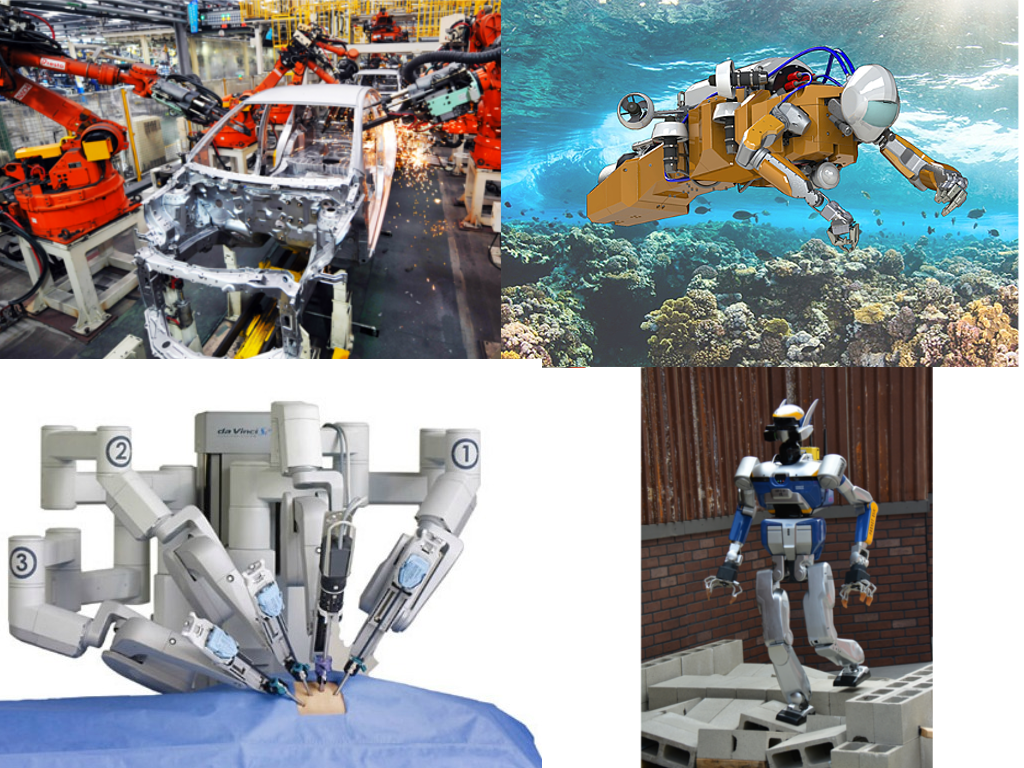
\includegraphics[width=0.9\textwidth]{various-tasks.png}
  \caption{Various robots doing various tasks}
\label{fig:various}
\end{figure}

The DARPA Robotics Challenge has shone some light on the humanoid robots.
This competition brought together a large scope of robotics groups from universities, laboratories and private companies around a common goal: teleoperate a robot to make it succeed in several challenges without any human physical intervention.
The robots were expected to drive a car, open a door, climb stairs, cross debris, drill a hole in a wall, etc.
All those tasks can usually be broken down into sets of elementary tasks in human language.
Some typical examples of tasks for a robot can be `Put hand in contact with target', `Put foot on next step', `Avoid collision with that object', `Maintain stability' or `Look in that direction'.
As is, those tasks do not mean anything for the robot.
A robot is made of a collection of bodies that are linked together by joints actuated by motors.
A robots configuration consists of the position and orientation of its base body, and the configuration of each of its joints.
Satisfying a task requires that the joints of the robot reach a configuration for which the task is satisfied.
The action of satisfying a task comes down to moving from an initial configuration to a goal.
Computing the trajectory to follow and actually following it are the jobs of the trajectory generation and the control of the robot.
Those are by themselves some complete fields of robotics, and they have one thing in common, they both need to be given an initial and a final configuration, and sometimes some intermediate ones.
Finding those configurations is the job of what we call the Posture Generator (PG).

There are two types of robots. The fixed-base robots and the mobile ones.
The first type of robots have fixed basis, the area that they can reach is predefined by their geometry and they are usually fully actuated.
This means that the robot has as many degrees of freedom (DoF) as actuators, Thus, for any joint configuration, a unique robots position can be achieved.
On the contrary, mobile robots are always underactuated, the robot has more DoF than actuators.
Each link of the robot is actuated, but the position of the basis of the robot depends on the configuration of the joints as a well as on the locations of the contacts that the robot makes with the environment.

%A mobile robot's position depends on the location of its contacts with the environment.
%For biped robots evolving on a flat surface, a footstep planner can be used to decide of the sequence of steps to take so the robot can walk to its goal.

Humanoid robots are expected to move and achieve tasks in ways similar to humans.
On flat surfaces, they can walk based on a cyclic motion and the locations of footsteps can be generated by a footstep planner using some simplified models to maintain the robots stability.
In cumbersome and unstructured environments, we humans move in a non-gaited acyclic way: we choose appropriate parts of our body to create contacts with the surrounding environment in order to support the motion of the remaining parts while avoiding obstacles.
A whole motion is a sequence of contact creations and releases.

Since we are biped, we mostly use our feet to move.
As the environment becomes more difficult to cross, hands may come into play together with feet to help with the motion.
Narrow passages may even require other parts of our body (knees, elbows, back\dots) to make contact in order to support the motion.

Planning the sequence of contacts to achieve is a necessary step in devising a motion for a robot.
Once the key stances of the motion have been identified by the planner, they can be used by the controller or the trajectory planner and finally the motion can be achieved by the robot.

All the aforementioned planning methods rely on the fact that we have a tool to decide if a proposed set of contacts is feasible or not for the robot.
The tool used for finding a robot configuration that satisfies a set of various constraints like the geometric constraints of contact or the stability of the robot is called a `Posture Generator' (PG) and the development of that tool is the main topic of this dissertation.

The mission of a posture generator is, for a polyarticulated system, to find a configuration so that the system satisfies a set of constraints.
For simple systems, with simple constraints, like a 6 DoF robotic arm having to reach a point with its end effector, some closed-form expressions can sometimes be devised.
But computing robot configuration to meet the requirements of a given set of tasks, within a viable state, is a recurrent problem whose complexity grows with that of the robot.
When the robotic problem studied becomes too complex for closed-form formulas, it is formulated as a nonlinear optimization program and solved using optimization algorithms.
The Posture Generator is a key tool of many robotics applications and as such, it is an important component of any robotics framework.
It needs to be efficient at finding a solution when one exists and at figuring when a problem is not feasible.
The speed of generating a multi-contact sequence is directly related to the quality of the posture generator, which is directly related to the quality of the optimization algorithm that it uses.

The variables of a robotics problem sometimes naturally belong to a non-Euclidean manifold $\mathcal{M}$, like $SO(3)$ for the 3D rotation of the base of a mobile robot.
A manifold is a topological space that locally resembles Euclidean space near each point.
Each point of an n-dimensional manifold has a neighbourhood that is homeomorphic to the Euclidean space of dimension n.
An n-dimensional non-Euclidean manifold cannot always be globally parameterized over a subset of $\mathbb{R}^n$ without presenting problems of singularity.
Most of the optimization solvers available make the assumption that the search space is Euclidean and thus, do not feature the capability of solving problems on non-Euclidean manifolds natively.
But it is often possible to parametrize $\mathcal{M}$ over a higher dimensionality Euclidean space with added constraint (e.g. unit quaternions, rotation matrices).
It is then possible to solve those problems with classical solvers at the cost of additional variables, constraints and special treatments in the optimization problem.
There exists some methods and algorithms to solve optimization problems on non-Euclidean manifolds with no substantial extra cost and guaranteeing a good coverage of the manifolds without facing parameterization singularities and with the minimal number of parameters, though to our knowledge, they are focused on non-constrained optimization.

%Usually, the solver used for solving optimization problems is a black box on which the user has a very limited control.
During this thesis, we develop our own nonlinear constrained optimization solver on manifolds, that we use to solve optimization problems on their native search manifolds, should they be posture generation problems or others.
This has the added advantage that unlike off-the-shelf solver, which are often a black box on which the user has a very limited level of control, we have full control over that solver and can specialize/modify it to fit our needs.

%\paragraph{Specificities of our approach}
%If we consider a problem of posture generation on a mobile robot with $n$ joints, the configuration space of the joints of the robot is $\mathbb{R}^n$ and the configuration space of the position and orientation of its base body is $SE(3) = \mathbb{R}^3\times SO(3)$.
%Thus, the variable that describes the configuration of the robot in the optimization problem lives in $\mathbb{R}^3\times SO(3) \times \mathbb{R}^n$.
%$SO(3)$ is by nature a non-Euclidean manifold, it cannot be parameterized on an open subset of Euclidean space without having to deal with problems of gimbal lock.
%The gimbal lock is a singularity that happens when parameterizing $SO(3)$ on $\mathbb{R}^3$, with Euler angles, for example, and when two axis of rotation become aligned, in that situation, 2 elements of the parameterization correspond to the same rotation.
%Thus, one degree of freedom is lost.
%Note that this singularity can block the optimization algorithm and that it is only due to the choice of parameterization, it is not intrinsic to the manifold $SO(3)$.
%It is possible to parameterize $SO(3)$ without having to face singularities by parameterizing it over another non-Euclidean manifold.
%The most common ones are the unit quaternion space and the $3\times 3$ rotation matrix.
%Most of the solvers available make the assumption that the search space is Euclidean, which makes is complicated to use quaternion or rotation matrix efficiently.
%To put it simply, for the unit quaternion parameterization, a variable on $SO(3)$ is represented by 4 parameters, the coefficients of the quaternion and an equality constraint needs to be added to the optimization problem to ensure that the quaternion is of norm 1, $\{q\in\mathbb{R}^4:||q||=1\}$.
%Similarly, if a variable is parameterized by a rotation matrix, then the variable $M$ has 9 parameters and several constraints need to be added to the problem so that M is symmetric, positive definite and its determinant is 1 $\{M\in\mathbb{R}^{3\times 3}:M^T M = \mathbb{I}_3\  \&\ \det (M) = 1\}$.
%Similar issues can be found with the parameterization of other non-Euclidean manifold, like $S2$ for example.

%There exists some methods and algorithms to solve optimization problems on non-Euclidean manifolds with no substantial extra cost and guaranteeing a good coverage of the manifolds without facing parameterization singularities and with the minimal number of parameters, though to our knowledge, they are focused on non-constrained optimization.

\paragraph{Contributions and plan}
The main focus of this thesis is the formulation and resolution of problems of posture generation for robotics systems using nonlinear optimization on manifolds.
Our contributions are of two types, on one hand we propose some extensions and improvements on the way to formulate a posture generation problem, and on the other hand, we investigate new ways of solving those problems.
The organization of this thesis is as follows:
%In Chapters~\ref{cha:state_of_the_art} and~\ref{cha:posture_generation_problem_formulation}, we present the background of posture generation, with respectively a state of the art and a presentation of the detailed formulation of a posture generation problem.
%We present several
\begin{itemize}
  \item In Chapter~\ref{cha:state_of_the_art_and_problem_definition} we give the state of the art of posture generation and optimization on manifolds.
  \item In Chapter~\ref{cha:posture_generation_problem_formulation}, we present the detailed formulation of a posture generation problem.
  \item In Chapter~\ref{cha:extensions_of_posture_generation} we present three different and unrelated contributions: two formulation extensions, one allowing to generate non-inclusive contacts between convex surfaces, the other is the exact derivation of the torques in the actuators of a robot.
  Then we present our endeavor to use the `Lifted Newton Method' to solve posture generation problems.
  \item Chapter~\ref{chapter:optimization_on_noneuclidean_manifolds} describes the principles of nonlinear optimization over non-Euclidean manifolds and our implementation of a solver based on those principles.
  \item In Chapter~\ref{ch:PG}, we present a framework that simplifies and extends the formulation of posture generation problems by formulating and solving the optimization problem over native non-Euclidean manifolds, managing automatically the variables of the problems and proposing a framework that formalizes and simplifies the writing of functions on geometric entities often used in robotics.
  \item In Chapter~\ref{cha:evaluation_and_experimentation}, we evaluate the performances of our solver on manifolds and of our posture generator, and then present a preliminary work on how to generate postures on a sensory acquired environment.
\end{itemize}




%%%%%%%%%%%%%%%%%%%%%%%%%%%%%%%%%%%%%%%%%%%%%%%%%%%%%%%%%%%%%%%%%%%%%%%
%                            First Chapter                            %
%               State of the Art of Posture Generation                %
%%%%%%%%%%%%%%%%%%%%%%%%%%%%%%%%%%%%%%%%%%%%%%%%%%%%%%%%%%%%%%%%%%%%%%%

\chapter{State of the Art of Posture Generation}
\label{cha:state_of_the_art_of_posture_generation}

\nomenclature[z-PG]{PG}{Posture Generation}
\nomenclature[z-IK]{IK}{Inverse Kinematics}
\nomenclature[z-DoF]{DoF}{degrees of freedom}
\nomenclature[x-I]{$\mathbb{I}_n$}{Matrix identity of dimension $n$}
\nomenclature[x-w]{$\wedge$}{cross product}
\nomenclature[z-mbg]{mbg}{Multibody Graph}
\nomenclature[a-F]{F}{a frame}
\nomenclature[a-W]{W}{the world frame}
\nomenclature[a-w]{w}{a wrench or a force}
\nomenclature[a-f]{f}{a force resultant}
\nomenclature[a-m]{m}{a force moment}


\graphicspath{{Chapter1-PG/Figs/Vector/}{Chapter1-PG/Figs/}}

%{{{List of contributions
%\section{List of contributions}

%%%%%%%%%%%%%%%%%%%%%%%%%%%%%%%%%%%%%%%%%%%%%%%%%%%%%%%%%%%%%%%%%%%%%%%%
%%                   SECTION LIST OF CONTRIBUTIONS                     %
%%%%%%%%%%%%%%%%%%%%%%%%%%%%%%%%%%%%%%%%%%%%%%%%%%%%%%%%%%%%%%%%%%%%%%%%

%\begin{itemize}
  %\item Generalities, introduction
  %\item Presentation of the existing methods
  %\item From Inverse Kinematics to Generalized IK/posture Generation/pose estimation (addition of articular limits, forces, stability etc).
  %\item Topology of the parametrization space (Free-flyer, q, f, other)
  %\item Formulation as a non-linear constrained optimization problem
  %\item Adrien \& Karim's formulations
  %\item Formulation of several types of cost/constraints
  %\begin{itemize}
    %\item Contact with planar surface
    %\item Collision avoidance
    %\item Auto-Collision avoidance
    %\item Static equilibrium: Newton/CoM projection
    %\item Forces in friction cones
    %\item Articular limits
    %\item Torque limits
    %\item Torque minimization
    %\item Goal Posture
  %\end{itemize}
  %\item Reasons why it is not enough and why we needed a new PG
    %\begin{itemize}
      %\item Having an easier way to formulate problems
      %\item Avoid having to de some gymnastic to remain on manifolds
      %\item Automatic variable management
      %\item Robustness
    %\end{itemize}
  %\item Utilization of posture generation in planning
%\end{itemize}
%}}}
%{{{SECTION:PROBLEM DEFINITION
\section{Problem Definition}
\label{sec:problem_definition}

%%%%%%%%%%%%%%%%%%%%%%%%%%%%%%%%%%%%%%%%%%%%%%%%%%%%%%%%%%%%%%%%%%%%%%%
%                     SECTION PROBLEM DEFINITION                      %
%%%%%%%%%%%%%%%%%%%%%%%%%%%%%%%%%%%%%%%%%%%%%%%%%%%%%%%%%%%%%%%%%%%%%%%

We consider the problem where we have a robotic system and we want to have it do some tasks, like for example to make a contact between a point on a body of the robot and a point of the environment.
This contact task can be modelized as a simple equality.
We denote $q$ the joint parameters of the robot, $g(q)$ is the 3D position of the point of interest on the robot and $P$ is the point of the environment.
Then our problem comes down to finding a configuration $q^*$ such that $f(q^*) = P$.
For complicated robots like humanoids, the equations describing its kinematics are quite complicated, and the presence of angular joints in the robotic system imply the non-linearity of those equations.
In the general case, even for simple tasks, a closed form solution of the problem does not exist.

We denote $\mathcal{C}$ the configuration space of our robotic system. It is the manifold in which $q$ lives. The dimension of $\mathcal{C}$ for a single robot in equal to the number of degrees of freedom of the robot. Note that if all the joints of the robot are actuated, this is the number of motors of the robot. And if the robot has a free-floating basis (is not fixed) then the position in $\mathcal{R}^3$ and rotation in $SO(3)$ of its basis are to be added to $q$.

We can formulate that problem as follows:

\begin{equation}
  \text{find}\ q\in\mathcal{C}\ \text{such that}\ g(q)=P
\end{equation}

The space of solution of this problem is a submanifold of $\mathcal{C}$ of lower dimension that we call ${\mathcal{C}}_F$ the feasible configuration space (which can be empty).

In addition to the equality constraint abovementioned, the problem can feature some inequality constraints.
For example, each joint variable can be limited to a certain range of value: $\forall i,\ q_i\in [q_i^-,\ q_i^+]$. Then the problem becomes a combination of equality and inequality constraints, and can be written as:
\begin{equation}
  \text{find}\ q\in\mathcal{C}\ \text{such that}\left\{
  \begin{array}{l}
    g(q)=P \\
    \forall i,\ q_i^- \leq q_i \leq q_i^+
  \end{array}
  \right.
\end{equation}

Finally, we can also require finding the point of $\mathcal{C}_F$ that minimizes a criterion, such as the distance to a goal posture $q_0$ for example.
Our problem becomes:

\begin{equation}
  \left\{
  \begin{array}{l}
    \min\limits_{q\in\mathcal{C}}{\|q-q_0\|_2}\\
    \text{ s.t. }
    \left\{
    \begin{array}{l}
      g(q)=P\\
      \forall i,\ q_i^- \leq q_i \leq q_i^+
    \end{array}
    \right.
  \end{array}
  \right.
\end{equation}

This type of problem is called a nonlinear constrained optimization problem and can be formulated in a more generic fashion as:

\begin{equation}
\label{eq:optim_form_PG}
  \left\{
  \begin{array}{l}
    \min\limits_{x\in\mathcal{C}}{f(x)}\\
    \text{ s.t. }
    \left\{
    \begin{array}{l}
      c_i(x) = 0,\ \forall i\in{E}\\
      c_i(x) \geq 0,\ \forall i\in{I}\\
    \end{array}
    \right.
  \end{array}
  \right.
\end{equation}

Where $x$ is the optimization variable in space $\mathcal{C}$ that we want to find, such that it minimizes the cost function $f(x)$ while satisfying all the equality constraints $c_i(x) = 0,\ \forall i\in{E}$ and inequality constraints $c_i(x) \geq 0,\ \forall i\in{I}$

Such problems can be solved by a Non-linear optimization solver.
In Appendix~\ref{chapter:optimization}, we present some principles of nonlinear optimization in unconstrained and constrained cases.
Several off-the-shelf solvers are available and have been widely used in for solving robotics problems.
The CFSQP solver~\cite{cfsqp:manual} was used in~\cite{escande:iros:2009} and~\cite{escande:ras:2013} where thousands of HRP-2 posture generation queries were made to explore the feasible space.
The IPOPT solver has been used in~\cite{vaillant:humanoids:2014},~\cite{vaillant:autonomousrobots:2016},~\cite{bouyarmane:ar:2012} where the posture generator had been extended to handle multi-robot problems and more complex and various contact models.
In this thesis, we use those off-the-shelf solvers a little in the beginning and later we tackle the development of our own non-linear optimization solver.

From this point forward, we formulate and solve posture generation problems as nonlinear constrained optimization problem. And in the next sections, we focus on the formulating several robotics constraints and cost function in the formalism of nonlinear optimization.
%}}}
%{{{SECTION:PROBLEM FORMULATION
\section{Problem Formulation}
\label{sec:pg_formulation}

%%%%%%%%%%%%%%%%%%%%%%%%%%%%%%%%%%%%%%%%%%%%%%%%%%%%%%%%%%%%%%%%%%%%%%%
%                    SECTION PROBLEM FORMULATION                      %
%%%%%%%%%%%%%%%%%%%%%%%%%%%%%%%%%%%%%%%%%%%%%%%%%%%%%%%%%%%%%%%%%%%%%%%

%{{{SUBSECTION:FORWARD KINEMATICS
\subsection{Forward Kinematics}
\label{sub:forward_kinematics}

%%%%%%%%%%%%%%%%%%%%%%%%%%%%%%%%%%%%%%%%%%%%%%%%%%%%%%%%%%%%%%%%%%%%%%%
%                   SUBSECTION FORWARD KINEMATICS                     %
%%%%%%%%%%%%%%%%%%%%%%%%%%%%%%%%%%%%%%%%%%%%%%%%%%%%%%%%%%%%%%%%%%%%%%%

In this section, we present a formulation of robotic systems that allows specifying most of the typical constraints encountered in robotics problems.

We consider a robotic system made of $n_B$ bodies and $n_J$ joints.
The global structure of the robot is described by an ordered graph called $mbg$ multi-body graph.
The base body (World) has index $0$ and other bodies get different positive integer index, we denote the body of index $i$, $B_i$. And $B_0$ can be called $B_W$.
Each body $B_i$ has its reference frame $F_i$ attached to it.
$F_0$ or $F_W$ denotes the World frame.
Bodies are linked together by joints that also are indexed by positive integers, we denote the joint of index $i$, $J_i$, and the body that comes after it is $B_i$.
Each joint defines the relation between its predecessor and successor bodies, for joint $J_i$ they are respectively denoted $pred(i)$ and $i$, and $B_{pred(i)}$ is called the parent body of $B_{i}$.
We denote $\lambda(j)$ the index of the parent body of $B_j$.
The number of degrees of freedom of $J_i$ is denoted $dof^J_i$ and the number of degrees of freedom of the whole robot is denoted $dof$.
Figure~\ref{fig:mbg} illustrates this numbering system for a simple robot with 4 joints and 5 bodies (including the basis)

\begin{figure}
  \centering
  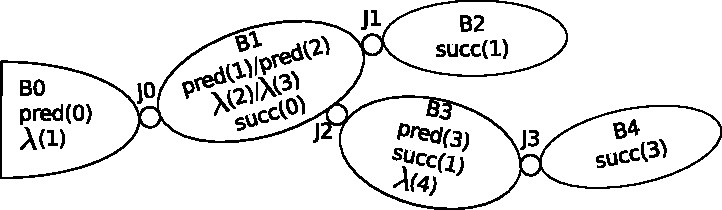
\includegraphics[width=0.7\textwidth]{mbg.pdf}
  \caption{MultiBody graph}
\label{fig:mbg}
\end{figure}

The geometric relations between bodies and joints are described through transformations between their reference frames. Each body $B_i$ has a reference frame $F_i$ attached to it. Transformations are described in the Spacial Vector Algebra chapter of `Rigid Body Dynamics Algorithm' by Roy Featherstone~\cite{featherstone:book:2007}.

For any 3D vector $v\in\mathbb{R}^3$, $\hat(v)$ denotes the $3\times 3$ skew-symmetric matrix such that $\hat{v}u = v\wedge u$. Where $\wedge$ denotes the cross product operator.

Let A and B be Cartesian frames with origins O and P respectively. Let $\mathbf{t}$ be the coordinate vector expressing $\overrightarrow{OP}$ in A. And $\mathbf{R}$ be the rotation matrix that transforms 3D vectors from A to B coordinates.
The transformation from A to B for a motion vector is defined by:
\begin{equation}
  {}^B X_A =
  \begin{bmatrix}
    \mathbf{R} & \mathbf{0} \\
    -\mathbf{R}\hat{\mathbf{t}} & \mathbf{R} \\
  \end{bmatrix}
\end{equation}
Its inverse is:
\begin{equation}
  {{}^B X_A}^{-1} = {}^A X_B =
  \begin{bmatrix}
    \mathbf{R}^T & \mathbf{0} \\
    \hat{\mathbf{t}}\mathbf{R}^T & \mathbf{R}^T \\
  \end{bmatrix}
\end{equation}
The transformation from A to B for a force vector is defined by:
\begin{equation}
  {}^B X_A^* =
  \begin{bmatrix}
    \mathbf{R} & -\mathbf{R}\hat{\mathbf{t}} \\
    \mathbf{0} & \mathbf{R} \\
  \end{bmatrix}
\end{equation}
Its inverse is:
\begin{equation}
  {}^B X_A^{-*} = {}^A X_B^* =
  \begin{bmatrix}
    \mathbf{R}^T & \hat{\mathbf{t}}\mathbf{R}^T \\
    \mathbf{0} & \mathbf{R}^T \\
  \end{bmatrix}
\end{equation}

%Each joint $J_i$ is defined in the reference frame of its predecessor body by a static transformation $X^x_i = \{\mathbf{R}^x_i, \mathbf{t}^x_i\}$ from the base of the body to the base of the joint.
Each joint $J_i$ is defined by a static transformation $X^x_i = \{\mathbf{R}^x_i, \mathbf{t}^x_i\}$ between the reference frame of its predecessor body and its own reference frame.
Each joint $J_i$ is associated with a motion subspace which representation matrix is denoted $\mathbf{S}_i$. Each column of $\mathbf{S}_i$ described a degree of freedom of $J_i$ its upper part for the rotations and lower for translations.
\begin{equation}
  \mathbf{S}_i =
  \begin{bmatrix}
    S^R_{i,0} & \cdots &
    S^R_{i,j} & \cdots &
    S^R_{i,dof} \\
    S^t_{i,0} & \cdots &
    S^t_{i,j} & \cdots &
    S^t_{i,dof}
  \end{bmatrix}
\end{equation}

For a given joint configuration $q$, the transformation due to the joint $J_i$ current configuration from its reference frame to the reference frame of its successor body is denoted \\$X^J_i (q) = \{\mathbf{R}^J_i (q), \mathbf{t}^J_i (q)\}$.

The transformation between $B_{\lambda(i)}$ and $B_i$ is denoted $X^{PtS}_i (q) = \{\mathbf{R}^{PtS}_i, \mathbf{t}^{PtS}_i\}$ (PtS stands for `Parent to Son') can then be computed as:
\begin{equation}
  {X}^{PtS}_i (q) = {}^{i}X_{\lambda (i)} (q) = X^J_i (q) X^x_i
  \label{eq:PtS}
\end{equation}

Let $\kappa (i) =\{0, i_1, i_2 \ldots i\}$ be the list of indexes of successive joints going from $B_W$ to $B_i$.
It can easily be computed by adding iteratively the parent of the current body:

\begin{algorithm}
  \caption{Joint Path to $B_i$}
\label{alg:JP}
\begin{algorithmic}
  \State{$j \leftarrow i$, $\kappa(i)=[i]$}
  \While{$j \neq 0$}
  \State{$j \leftarrow \lambda(j)$}
  \State{$\kappa(i) \leftarrow [\kappa(i),\ j]$}
  \EndWhile{}
\end{algorithmic}
\end{algorithm}

The transformation from the World base to $B_i$ is denoted \\ ${}^i X_W (q) = \{{}^i \mathbf{R}_W (q), {}^i \mathbf{t}_W (q)\}$.
The formula~\ref{eq:PtS} can be used iteratively on every body of the robot to obtain the expression of ${}^i X_W (q)$.

We obtain the full expression of ${}^i X_W$ as:
\begin{equation}
  {}^i X_W (q) = \prod_{j\in\kappa (i)}X^J_j (q) X^x_j = \prod_{j\in\kappa (i)}\ {}^j X_{\lambda (j)}
  = {}^i X_{\kappa (1)}\ ^{\kappa (1)}X_{\kappa (2)} \dots ^{\kappa (\text{end}-1)}X_{W}
\end{equation}

Which can be computed recursively by a Forward Kinematics algorithm:

\begin{algorithm}
  \caption{Forward Kinematics}
\label{alg:FK}
\begin{algorithmic}
  \For{$i = 0:n_J$}
  \If{$\lambda (i) \neq -1$} ${}^i X_W = {}^i X_{\lambda (i)}\ ^{\lambda (i)}X_W$
  \Else$\ {}^i X_W = X^{PtS}_i$
  \EndIf{}
  \EndFor{}
\end{algorithmic}
\end{algorithm}

In the following section, we provide some detailed description of how to compute $X_J (q)$ for a variety of useful joints.
Using the joint descriptions and the Forward Kinematics algorithm, we are able to explicit a relation between $q$ the joint parameters of the robot and the 3D position and orientation of  any geometric quantity defined in the reference frame of a body of the robot.
Given a transformation ${}^p X_i$ defined in the frame of $B_i$, its value in the world frame is given by ${}^p X_W (q) = {}^p X_i\ {}^i X_W (q)$
%}}}
%{{{SUBSECTION:JOINTS FORMULATIONS
\subsection{Joints formulations}
\label{sub:joints_formulations}

%%%%%%%%%%%%%%%%%%%%%%%%%%%%%%%%%%%%%%%%%%%%%%%%%%%%%%%%%%%%%%%%%%%%%%%
%                   SUBSECTION JOINTS FORMULATIONS                    %
%%%%%%%%%%%%%%%%%%%%%%%%%%%%%%%%%%%%%%%%%%%%%%%%%%%%%%%%%%%%%%%%%%%%%%%

The entire geometry of our system is described by the list of static transformations $X^x_j$ and of joint transformations $X^J_j (q)$.
In this section, we explicit the descriptions and formulations of several useful joints.

Let us consider a joint $J$ that governs the transformation between two frames $F_1=\{O_1, x_1, y_1, z_1\}$ and $F_2=\{O_2, x_2, y_2, z_2\}$.
The most common type of joint encountered in robotics systems is the revolute joint, that allows a rotation around a fixed axis.
If $J$ is a revolute joint around the axis $(O_1,z_1)$ with parameter $q$, its motion subspace, rotation and translation are as follows:

\begin{table} [ht]
\centering
\begin{tabular}{cccc}
  \toprule
  Joint type & $S$ & $Rotation$ & $translation$ \\
  \midrule
  Revolute $(O_1,z_1)$
  &
  $\begin{bmatrix}
    0 \\ 0 \\ 1 \\ 0 \\ 0 \\ 0
  \end{bmatrix}$
  &
  $\begin{bmatrix}
    1 & 0 & 0 \\
    0 & \cos (q) & \sin (q) \\
    0 & -\sin (q) & \cos (q) \\
  \end{bmatrix}$
  &
  ${\bf 0}_{3\times1}$
  \\
  \bottomrule
\end{tabular}
\end{table}

Similar formulas can be devised for rotations around any other axis, provided that $R$ describes the rotation of angle $q$ around that axis.

In the case of a prismatic joint, all rotations are blocked, and only one translation along a given axis is allowed.
A prismatic joint along $x_1$ is described by the following formulas:

\begin{table} [ht]
\centering
\begin{tabular}{cccc}
  \toprule
  Joint type & $S$ & $Rotation$ & $translation$ \\
  \midrule
  Prismatic $(x_1)$
  &
  $\begin{bmatrix}
    0 \\ 0 \\ 0 \\ 1 \\ 0 \\ 0
  \end{bmatrix}$
  &
  ${\bf 1}_{3\times3} $
  &
  $\begin{bmatrix}
    q \\ 0 \\ 0
  \end{bmatrix}$
  \\
  \bottomrule
\end{tabular}
\end{table}

Planar joints are also frequently used in robotics.
A planar joint describes a plan sliding on another plan, assuming that the normal to both plans is $z_1 = z_2$ this type of joint allows free rotation of $F_2$ around $z_1$ and translations along $x_1$ and $y_1$. We denote $q = \{q_1, q_2, q_3\}$ the joint parameters, $q_1$ corresponding to the rotation and $q_2,\ q_3$ to the translations. We get:

\begin{table} [ht]
\centering
\begin{tabular}{cccc}
  \toprule
  Joint type & $S$ & $Rotation$ & $translation$ \\
  \midrule
  Planar $(z_1)$
  &
  $\begin{bmatrix}
    0 & 0 & 0 \\ 0 & 0 & 0 \\ 1 & 0 & 0 \\ 0 & 1 & 0 \\ 0 & 0 & 1 \\ 0 & 0 & 0
  \end{bmatrix}$
  &
  $\begin{bmatrix}
    1 & 0 & 0 \\
    0 & \cos(q_1) & \sin(q_1) \\
    0 & -\sin(q_1) & \cos(q_1) \\
  \end{bmatrix}$
  &
  $\begin{bmatrix}
    \cos(q_1)q_2 - \sin(q_1)q_3 \\ \sin(q_1)q_2 + \cos(q_1)q_3 \\ 0
  \end{bmatrix}$
  \\
  \bottomrule
\end{tabular}
\end{table}

A spherical joint blocks all translations and allows all rotations. This joint must be parameterized by a 3D rotation. The space of 3D rotations $SO(3)$ can be represented in many different ways.
The simplest and most intuitive way to parameterize $SO(3)$ is to use Euler Angles.
It comes down to decomposing the 3D rotation into a succession of three 1D rotations around different axes.
For example, the roll, pitch, yaw is a succession of a rotation of $F_1$ around its $x$ axis, followed by a rotation of the resulting frame around its $y$ axis and a rotation of the resulting frame around its $z$ axis.
The rotation matrix for such a rotation is given by:
\begin{equation}
  {\bf R} =
  \begin{bmatrix}
    1 & 0 & 0 \\
    0 & \cos(q_3) & \sin(q_3) \\
    0 & -\sin(q_3) & \cos(q_3) \\
  \end{bmatrix}
  +
  \begin{bmatrix}
    \cos(q_2) & 0 & -\sin(q_2) \\
    0 & 1 & 0 \\
    \sin(q_2) & 0 & \cos(q_2) \\
  \end{bmatrix}
  +
  \begin{bmatrix}
    \cos(q_1) & \sin(q_1) & 0 \\
    -\sin(q_1) & \cos(q_1) & 0 \\
    0 & 0 & 1
  \end{bmatrix}
\end{equation}

There are many other possible choices of axes to define the a Euler Angle 3D rotation.
This formulation has the advantage to be simple and intuitive.
But they all suffers from singularities like the Gimbal lock, which happens when two of the three rotation axis become aligned.
In such a configuration, the only rotations possible are one rotation around the two aligned axis and one rotation around the third axis.
Thus, one degree of freedom is lost.
Those singularities are prohibitive for the use of such a formulation in a posture generation (the optimization algorithm could get stuck in them).

One can prove that there is no smooth mapping between $SO(3)$ and $\mathbb{R}^3$ that is free of singularities.
The most common $SO(3)$ representation in robotics uses the subset of $\mathbb{R}^4$ called the unit quaternion.
A quaternion $q = [q_w, q_x, q_y, q_z]$ is a unit quaternion iff $q_w^2+q_x^2+q_y^2+q_z^2 = 1$.
It represents a rotation of angle $\theta$ around an axis ${\bf u}$ such that:
\begin{align}
  q_w &= \cos(\theta/2) \\
  q_x &= \sin(\theta/2)u_x \\
  q_y &= \sin(\theta/2)u_y \\
  q_z &= \sin(\theta/2)u_z \\
\end{align}
The rotation matrix associated with this quaternion is:
\begin{equation}
  {\bf R} = 2 \begin{bmatrix}
    q_w^2 +q_x^2-\frac{1}{2} & q_x q_y + q_w q_z & q_x q_z - q_w q_y \\
    q_x q_y - q_w q_z & q_w^2 +q_y^2-\frac{1}{2} & q_y q_z + q_w q_x \\
    q_x q_z + q_w q_y & q_y q_z - q_w q_x & q_w^2 +q_z^2-\frac{1}{2} \\
  \end{bmatrix}
\end{equation}

That formulation does not suffer from singularities, but it requires to maintain 4 parameters for a 3D rotation. And those 4 parameters must satisfy the unit norm constraint which in turn would become an additional constraint in the optimization formulation.
Given a parameter set $q = \{ q_w, q_x, q_y, q_z\}$, we get the following table.

\begin{table}[ht]
  \centering
  \begin{tabular}{cccc}
    \toprule
    Joint type & $S$ & $Rotation$ & $translation$ \\
    \midrule
    Spherical
    &
    $\begin{bmatrix}
      1 & 0 & 0 \\ 0 & 1 & 0 \\ 0 & 0 & 1 \\ 0 & 0 & 0 \\ 0 & 0 & 0 \\ 0 & 0 & 0
    \end{bmatrix}$
    &
    $2 \begin{bmatrix}
      q_w^2 +q_x^2-\frac{1}{2} & q_x q_y + q_w q_z & q_x q_z - q_w q_y \\
      q_x q_y - q_w q_z & q_w^2 +q_y^2-\frac{1}{2} & q_y q_z + q_w q_x \\
      q_x q_z + q_w q_y & q_y q_z - q_w q_x & q_w^2 +q_z^2-\frac{1}{2} \\
    \end{bmatrix}$
    &
    $\begin{bmatrix}
      0 \\ 0 \\ 0
    \end{bmatrix}$
    \\
    \bottomrule
  \end{tabular}
\end{table}

Finally, a free joint allows free motion of its successor body with respect to its predecessor body.
It can be viewed as a combination of a spherical joint and 3 perpendicular prismatic joints.
Given a parameter set $q = \{ q_w, q_x, q_y, q_z, t_x, t_y, t_z\}$, we get the following table.

\begin{tabular}{cccc}
  \toprule
  Joint type & $S$ & $Rotation$ & $translation$ \\
  \midrule
  Spherical
  &
  ${\bf 1}_{6\times 6}$
  &
  $2 \begin{bmatrix}
    q_w^2 +q_x^2-\frac{1}{2} & q_x q_y + q_w q_z & q_x q_z - q_w q_y \\
    q_x q_y - q_w q_z & q_w^2 +q_y^2-\frac{1}{2} & q_y q_z + q_w q_x \\
    q_x q_z + q_w q_y & q_y q_z - q_w q_x & q_w^2 +q_z^2-\frac{1}{2} \\
  \end{bmatrix}$
  &
  ${\bf R}^{-1}\begin{bmatrix}
    t_x \\ t_y \\ t_z
  \end{bmatrix}$
  \\
  \bottomrule
\end{tabular}

%}}}
%{{{SUBSECTION:JACOBIAN COMPUTATION

\subsection{Jacobian computation}
\label{sub:jacobian_computation}

%%%%%%%%%%%%%%%%%%%%%%%%%%%%%%%%%%%%%%%%%%%%%%%%%%%%%%%%%%%%%%%%%%%%%%%
%                  SUBSECTION JACOBIAN COMPUTATION                    %
%%%%%%%%%%%%%%%%%%%%%%%%%%%%%%%%%%%%%%%%%%%%%%%%%%%%%%%%%%%%%%%%%%%%%%%

For the sake of solving our problem with a non-linear optimization algorithm, it is necessary to compute the derivatives of every function used as constraint or cost with respect to any variable of the problem.
The transformations ${}^i X_W$ are used in many functions, therefore, having an efficient algorithm to compute their derivatives and the derivatives of any transformation defined in $B_i$ is necessary.

Let's consider a static transformation ${}^p X_i$ defined in body $B_i$.
Its expression in the world frame is ${}^p X_W = {}^p X_i\ {}^i X_W$ and its expression in the frame of $B_j$ is ${}^p X_j = {}^p X_i\ {}^i X_W\ {{}^j X_i}^{-1}$.

We denote $q_i$ the part of $q$ that corresponds to the degrees of freedom of joint $J_i$.
We denote $\text{Jac}_i.\text{cols}(j)$ the columns of $\text{Jac}_i$ associated with joint $J_i$.
The jacobian $B_i$ at ${}^p X_i$ with respect to $q_i$ is given by
\begin{equation}
\label{partial_jacobian}
  \text{Jac}_i.\text{cols}(j)({}^p X_i) = {}^p X_j\ S_i
\end{equation}

The complete jacobian of a body $\text{Jac}_i$ is a $6\times \text{dof}$ matrix that can be computed by using the formula~\ref{partial_jacobian} on every index $j$ in $\kappa(i)$ and filling the rest of $\text{Jac}_i$ with zeros.

The algorithm that we use to compute $\text{Jac}_i({}{}^p X_i)$ writes as follows:

\begin{algorithm}
  \caption{Jacobian Computation}
\label{Jacobian}
\begin{algorithmic}
  \State{$\text{Jac}_i({}^p X_i) = {\bf 0}_{6\times\text{dof}}$}
  \State{${}^p X_W = {}^p X_i\ {({}^i X_W)}^{-1}$}
  \For{$j = 0:\text{size}(\kappa(i))$}
  \State{$k \leftarrow \kappa(j)$}
  \State{${}^p X_k = {}^p X_W\ {({}^k X_W)}^{-1}$}
  \State{$\text{Jac}_i({}^p X_i).\text{cols}(k) = {}^p X_k\ S_k$}
  \EndFor{}
\end{algorithmic}
\end{algorithm}

We write the jacobian of each body at its origin as follows:
\begin{equation}
  \mathbf{Jac}^W_i = 
  \begin{bmatrix}
    \frac{\partial {}^i\mathbf{R}_W}{\partial q_0} & \cdots &
    \frac{\partial {}^i\mathbf{R}_W}{\partial q_j} & \cdots &
    \frac{\partial {}^i\mathbf{R}_W}{\partial q_{dof}} \\
    \frac{\partial {}^i\mathbf{t}_W}{\partial q_0} & \cdots &
    \frac{\partial {}^i\mathbf{t}_W}{\partial q_j} & \cdots &
    \frac{\partial {}^i\mathbf{t}_W}{\partial q_{dof}}
  \end{bmatrix}
= 
  \begin{bmatrix}
    \omega_{i,0} & \cdots &
    \omega_{i,j} & \cdots &
    \omega_{i,dof} \\
    v_{i,0} & \cdots &
    v_{i,j} & \cdots &
    v_{i,dof}
  \end{bmatrix}
\end{equation}
%}}}
%}}}
%{{{SECTION:GEOMETRIC CONSTRAINTS
\section{Geometric constraints}
\label{sec:geometric_constraints}

%%%%%%%%%%%%%%%%%%%%%%%%%%%%%%%%%%%%%%%%%%%%%%%%%%%%%%%%%%%%%%%%%%%%%%%
%          SECTION GEOMETRIC CONSTRAINTS                              %
%%%%%%%%%%%%%%%%%%%%%%%%%%%%%%%%%%%%%%%%%%%%%%%%%%%%%%%%%%%%%%%%%%%%%%%

%{{{SUBSECTION:JOINT LIMITS
\subsection{Joint Limits}
\label{sub:joint_limits}

%%%%%%%%%%%%%%%%%%%%%%%%%%%%%%%%%%%%%%%%%%%%%%%%%%%%%%%%%%%%%%%%%%%%%%%
%                      SUBSECTION JOINT LIMITS                        %
%%%%%%%%%%%%%%%%%%%%%%%%%%%%%%%%%%%%%%%%%%%%%%%%%%%%%%%%%%%%%%%%%%%%%%%

Most robotic joints have geometric limits which define the range of value that can be accessed by the joint variables.
The joint limits for 1D joints like revolute and prismatic joints are trivial to formulate: We denote $q^-$ and $q^+$ the lower and upper values accessible and add a boundary constraint to the optimization problem:
\begin{equation}
\label{eq:joint_limits}
  \boxed{q^- \leq q \leq q^+}
\end{equation}

Planar joints are easy to limit because their 3 variables are independent.
Each variable can be separately limited.
Limiting the movements of a spherical joint, and by extension, of a free joint, is more complicated.
In humanoid robotics, spherical joints can be used to model the shoulder or hip joint of the robot.
A common approach to limit shoulder joint, inspired from the biomechanics field, considers the spherical motion (or swing) and the axial motion (or twist) separately as shown in~\Figref{fig:ballAndSocket}.

\begin{figure}[htpb]
  \centering
  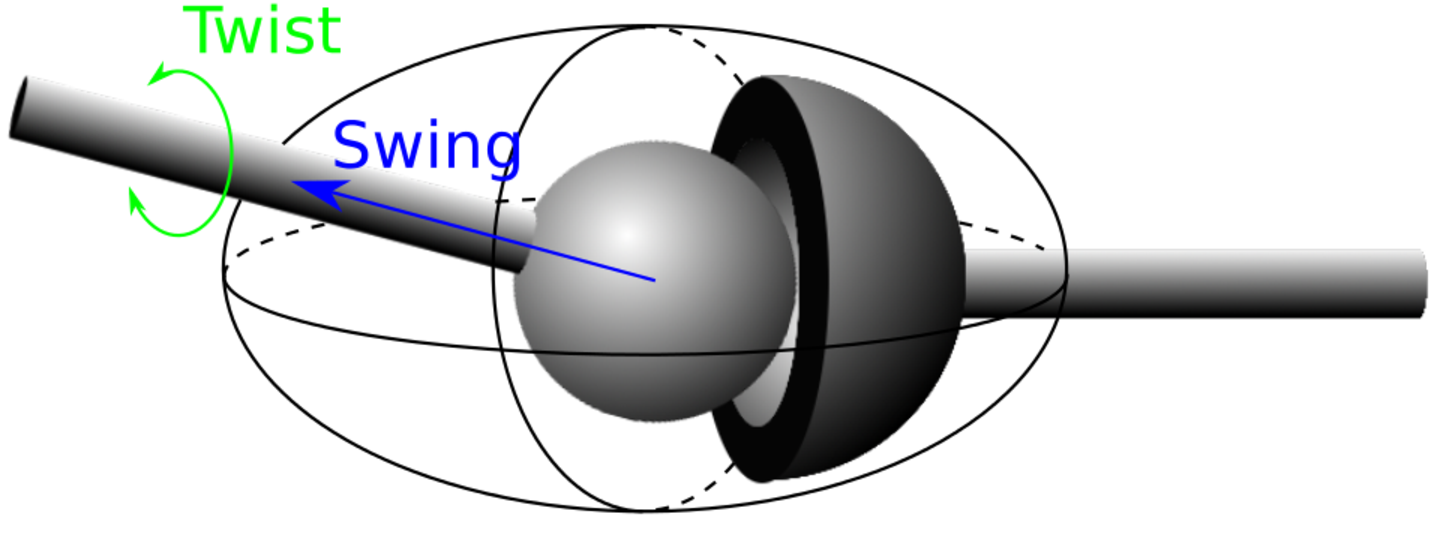
\includegraphics[width=0.7\linewidth]{ballAndSocket.pdf}
  \caption{Swing and Twist in ball and socket joint}
\label{fig:ballAndSocket}
\end{figure}

The spherical motion can be parameterized by a vector of the unit 3D sphere $S2$ and constrained to lay within a limit cone. And the axial motion can be parameterized in $\mathbb{R}$ and be limited by equation~\ref{eq:joint_limits}, this type of formulation is presented in~\cite{baerlocher}.

%}}}
%{{{SUBSECTION:CONTACT CONSTRAINTS
\subsection{Contact constraints}
\label{sub:contact_constraints}

%%%%%%%%%%%%%%%%%%%%%%%%%%%%%%%%%%%%%%%%%%%%%%%%%%%%%%%%%%%%%%%%%%%%%%%
%                   SUBSECTION CONTACT CONSTRAINTS                    %
%%%%%%%%%%%%%%%%%%%%%%%%%%%%%%%%%%%%%%%%%%%%%%%%%%%%%%%%%%%%%%%%%%%%%%%

Humanoid robots evolve in their environment by making and breaking contacts with it.
A contact can be defined between 2 surfaces of different bodies of robots (Note that one of the robots can be the environment or that the two robots can be the same).
The most usual type of contact constraint encountered is the planar contact, where a planar surface of a robot is put in contact with a planar surface of the environment.
We denote $F_1 = \{O_1, \vec{x_1}, \vec{y_1}, \vec{z_1}\}$ a frame defined on $S_1$, the surface of the first body involved in the contact, such that the 3D point $O_1$ is on $S_1$ and the vector $\vec{z_1}$ is normal to $S_1$ and pointing toward the inside the body.
$F2 = \{O_2, \vec{x_2}, \vec{y_2}, \vec{z_2}\}$ is a frame on $S_2$, the surface of the second body involved, such that $O_2$ is on $S_2$ and the vector $\vec{z_2}$ is normal to $S_2$ and pointing away from the body.

Constraining $S_1$ and $S_2$ to be coplanar comes down to aligning $\vec{z_1}$ and $\vec{z_2}$ and to ensure that the projection of the distance between $O_1$ and $O_2$ along $\vec{z_1}$ is null.
Note that we avoid using the dot product of two vectors that are meant to be aligned e.g. $\vec{z_1}\cdot\vec{z_2} = 1$ because when that constraint is satisfied, its gradient is null, which implies that in the optimization context it is unqualified.
That is why we prefer imposing orthogonality constraints.
This translates into adding the following set of constraints to our problem:

\begin{equation}
\label{eq:coplanarity}
\boxed{\left\{
  \begin{array}{l}
    \overrightarrow{O_1O_2} \cdot \vec{z_1} = 0\\
    \vec{x_1}\cdot\vec{z_2} = 0\\
    \vec{y_1}\cdot\vec{z_2} = 0\\
    \vec{z_1}\cdot\vec{z_2} \geq 0
  \end{array}
  \right.}
\end{equation}

This set of constraints leaves free the displacements of $F_2$ along $\vec{x_1}$ and $\vec{y_1}$ as well as its rotation around $\vec{z_1}$.
We call this a floating contact, the optimization algorithm will be able to choose the location of $F_2$ in the plane $\{O_1, \vec{x_1}, \vec{y_1}\}$. This contact has 3 degrees of freedom.

\begin{figure}[htpb]
  \centering
  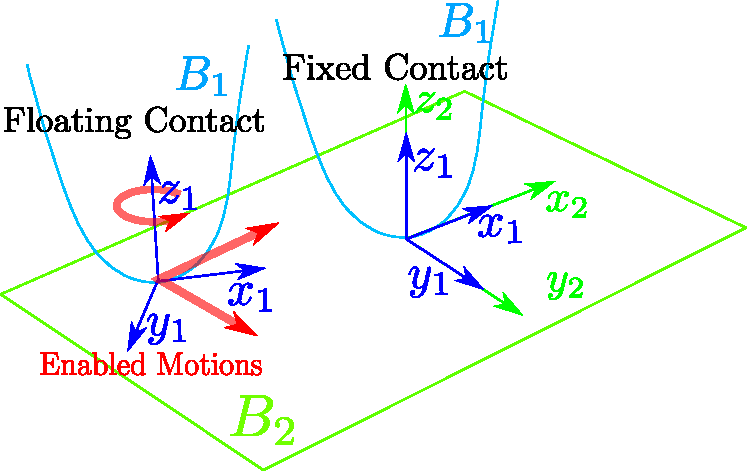
\includegraphics[width=0.8\linewidth]{contactConstraint.pdf}
  \caption{Floating and Fixed Contacts}
\label{fig:contactConstraint}
\end{figure}

If we constrain the location of $F_2$ in $\{O_1, \vec{x_1}, \vec{y_1}\}$ such that $O_1$ and $O_2$ superimposed and $\vec{x_1}$, $\vec{y_1}$, $\vec{z_1}$ are aligned respectively with $\vec{x_2}$, $\vec{y_2}$, $\vec{z_2}$, we obtain a fixed contact with no degree of freedom. This translates into adding the following set of constraints to our problem:

\begin{equation}
\label{eq:fixed_contact}
\boxed{\left\{
  \begin{array}{l}
    \overrightarrow{O_1O_2} = \vec{0}\\
    \vec{x_1}\cdot\vec{z_2} = 0\\
    \vec{y_1}\cdot\vec{z_2} = 0\\
    \vec{x_1}\cdot\vec{y_2} = 0\\
    \vec{z_1}\cdot\vec{z_2} \geq 0\\
    \vec{x_1}\cdot\vec{x_2} \geq 0\\
  \end{array}
  \right.}
\end{equation}

We illustrate those two types of contacts in~\Figref{fig:contactConstraint}
%}}}
%{{{SUBSECTION:COLLISION AVOIDANCE
\subsection{Collision avoidance}
\label{sub:collision_avoidance}

%%%%%%%%%%%%%%%%%%%%%%%%%%%%%%%%%%%%%%%%%%%%%%%%%%%%%%%%%%%%%%%%%%%%%%%
%                   SUBSECTION COLLISION AVOIDANCE                    %
%%%%%%%%%%%%%%%%%%%%%%%%%%%%%%%%%%%%%%%%%%%%%%%%%%%%%%%%%%%%%%%%%%%%%%%

In order to avoid unwanted collisions between bodies of robots, for two bodies $B_1$ and $B_2$, we want to define a continuously differentiable function $d_{\{B_1, B_2\}}(q)$ that has the properties of a pseudo-distance:
\begin{itemize}
  \item $d_{\{B_1, B_2\}}(q) > 0$ when the bodies are not touching each other
  \item $d_{\{B_1, B_2\}}(q) = 0$ when the bodies are in collision without interpenetration
  \item $d_{\{B_1, B_2\}}(q) < 0$ when the bodies are in collision with interpenetration
\end{itemize}

Using the cartesian distance between the exact surfaces of $B_1$ and $B_2$ might result in a discontinuous gradient of $d_{\{B_1, B_2\}}$ if the surfaces of $B_1$ and $B_2$ are not strictly convex.
A conservative approach is to associate to each body, a strictly convex bounding volume and to compute the distance between those volumes.
\cite{escande:humanoids:2007} and~cite{escande:itro:2014} proposes a method to generate a strictly convex Sphere-Torus-Patch Bounding Volumes (STP-BV) that guarantees the gradient continuity of the proximity distance.
The distance between the STP-BV of $B_1$ and $B_2$ computed by an enhanced GJK~\cite{gilbert-1988a} collision-detection algorithm is a continuously differentiable pseudo-distance.
Thus, we can use this function in our optimization algorithm as:

\begin{equation}
  \boxed{d_{\{B_1, B_2\}}(q) > 0}
\end{equation}

This function can be used to avoid collisions between a robot and the environment as well as auto collisions between bodies of the same robot.
We denote $Coll$ the list of triplets $\{B_i, B_j, \epsilon_{ij}\}$ defining each collision that we want to avoid by using this function in our problem, as a pair of bodies $B_i$ and $B_j$ and a minimal distance that we want to keep between them (usually for security reasons).

Then the set of constraints to add to our problem is:

\begin{equation}
  \boxed{\forall \{B_i, B_j, \epsilon_{ij}\} \in Coll,\ d_{\{B_i, B_j\}}(q) > \epsilon_{ij}}
\end{equation}

In many cases, it is possible to avoid the collision between two bodies of a robot by modifying the joint limits and reducing them to a span where the collision of interest cannot happen. That approach is conservative and ad-hoc but can save some precious computation time.
%}}}
%}}}
%{{{SECTION:STATIC CONSTRAINTS
\section{Static constraints}
\label{sec:static_constraints}

%%%%%%%%%%%%%%%%%%%%%%%%%%%%%%%%%%%%%%%%%%%%%%%%%%%%%%%%%%%%%%%%%%%%%%%
%                SECTION STATIC CONSTRAINTS                           %
%%%%%%%%%%%%%%%%%%%%%%%%%%%%%%%%%%%%%%%%%%%%%%%%%%%%%%%%%%%%%%%%%%%%%%%

%{{{SUBSECTION:EXTERNAL FORCES
\subsection{External Forces}
\label{sub:external_forces}

%%%%%%%%%%%%%%%%%%%%%%%%%%%%%%%%%%%%%%%%%%%%%%%%%%%%%%%%%%%%%%%%%%%%%%%
%                     SUBSECTION EXTERNAL FORCES                      %
%%%%%%%%%%%%%%%%%%%%%%%%%%%%%%%%%%%%%%%%%%%%%%%%%%%%%%%%%%%%%%%%%%%%%%%

For a robot to interact with the real world, its geometric description is not enough.
The robot is subject to forces applied on its bodies by the exterior world, those can be generated by contacts with the environment or with another actor (human, another robot, manipulated object\ldots), by the effect of physical forces like gravitation or magnetism, or by contacts between two bodies of the robot.
Our posture generator must take those `External forces' into account, be able to estimate the stability of the robot and compute the internal torques generated in the joints.

An external force applied on a rigid body can also be called a wrench and is composed of a resultant part $f$ (sometimes abusively called force) and a moment part (sometimes abusively called couple).
Let $w$ be a wrench, $w|_F^O$ is the expression of $w$ calculated at the point $O$ expressed in the frame $F$.
We denote $\vec{f}$ the resultant part of w, and $\vec{f}|_F$ the expression of $\vec{f}$ in $F$.
$\vec{m}$ is the moment part of $w$ and $\vec{m}|_F^O$ the expression of $\vec{m}$ in $F$ calculated at the point $O$.

\begin{equation}
  w|_F^O = \left\{ \begin{array}{r}
    \vec{m}\\
    \vec{f}\\
  \end{array} \right\}^O_F
  = \left\{ \begin{array}{r}
    \vec{m}|_F^O\\
    \vec{f}|_F\\
  \end{array}\right\}
\end{equation}

The expression of the moment part on a different point $P$ is given by the following formula:

\begin{equation}
  \vec{m}|_F^P = \vec{m}|_F^O + \overrightarrow{PO} \wedge \vec{f}|_F
\end{equation}

Whereas the resultant part is invariant with respect to the point at which the wrench is calculated.

Note that the frame subscript can be dropped in some equations where the choice of the frame does not matter and assuming that all the quantities of the equations are computed in the same frame.

%}}}
%{{{SUBSECTION:STATIC STABILITY
\subsection{Static stability}
\label{sub:static_stability}

%%%%%%%%%%%%%%%%%%%%%%%%%%%%%%%%%%%%%%%%%%%%%%%%%%%%%%%%%%%%%%%%%%%%%%%
%                    SUBSECTION STATIC STABILITY                      %
%%%%%%%%%%%%%%%%%%%%%%%%%%%%%%%%%%%%%%%%%%%%%%%%%%%%%%%%%%%%%%%%%%%%%%%

We denote $g$ the acceleration of gravity on earth $g = 9.81 m.s^{-2}$.
The wrench associated with the action of gravity on a body of mass $M$ which center of mass is denoted $G$ with $\vec{z}$ the upward vertical vector in the world frame $F_W$ is:
\begin{equation}
  w_g|^G_{F_W} = \left\{ \begin{array}{r}
     \vec{0} \\
     -Mg\vec{z} \\
 \end{array}\right\}^G_{F_W}
\end{equation}

A solid is statically stable if it satisfy the Euler-Newton Equation. We consider a robot on which $m$ external forces $w_i = \left\{ \begin{array}{r}
    \vec{m_i}\\
    \vec{f_i}\\
\end{array} \right\}^{P_i}$ are applied. We denote $P$ the application point on which the equation and all its terms are calculated:
\begin{equation}
  \sum\limits_i w_i|^P + w_g|^P = 0
\end{equation}
Which is equivalent to:
\begin{equation}
\left\{
\begin{array}{r}
  \sum\limits_i \vec{m_i}|^P + \overrightarrow{GP}\wedge Mg\vec{z} = 0 \\
  \sum\limits_i \vec{f_i} - Mg\vec{z} = 0 \\
\end{array}
\right.
\end{equation}

This equation can be simplified by applying it at the center of mass of the body as:
\begin{equation}
  \left\{
  \begin{array}{r}
    \sum\limits_i \vec{m_i}|^G = 0 \\
    \sum\limits_i \vec{f_i} - Mg\vec{z} = 0 \\
  \end{array}
  \right.
\label{eq:stability}
\end{equation}

Satisfying~\Eqref{eq:stability} ensures the stability of a rigid body.
In some cases, an articulated robot is considered as a rigid body and this equation alone can be used to ensure its stability.
It is only valid if the robot can generate infinite torques in its articulations, or at least if we have some guarantee that the robot is able to generate large enough torques.
Otherwise, it is necessary to verify that the robot's actuators can generate large enough torques to maintain that posture. The details of torque computation are discussed in Section~\ref{sub:torque_limits}

Equation~\ref{eq:stability} can be used in an optimization problem.
We consider that each wrench $w_i$ applied on the system is defined by the position of its application point $P_i$ and the values $m_i$ and $f_i$ that represent the moment and resultant of $w_i$ at $P_i$. $P_i$ depends on $q$ the joint parameter of the robot.
$m_i$ and $f_i$ are new variables that need to be added to the problem. In summary, $w_i$ depends on $q$, $m_i$ and $f_i$.
We denote $f$ the concatenation of all the variables $m_i$ and $f_i$.

\begin{equation}
  \boxed{s(q,f) = \left\{
  \begin{array}{r}
    \sum\limits_i \vec{m_i} + \overrightarrow{P_i G}\wedge \vec{f_i} \\
    \sum\limits_i \vec{f_i} - Mg\vec{z} \\
  \end{array}
  \right\}
  = 0}
\end{equation}

The optimization problem~\ref{eq:optim_form_PG} becomes (we denote m the dimension of the force variables):

\begin{equation}
\label{eq:optim_form_PG_with_stab}
  \left\{
  \begin{array}{l}
    \min\limits_{q\in\mathcal{C}, f\in \mathbb{R}^m}{f(q)}\\
    \text{ s.t. }
    \left\{
    \begin{array}{l}
      s(q,f) = 0\\
      c_i(q) = 0,\ \forall i\in{E}\\
      c_i(q) \geq 0,\ \forall i\in{I}\\
    \end{array}
    \right.
  \end{array}
  \right.
\end{equation}

The derivation of the static stability constraint is straightforward.
All the terms of equation~\ref{eq:stability} are components of wrenches.
A wrench is completely defined by the frame in which it is expressed and its values of resultant and moment in that frame.
Deriving the stability condition comes down to deriving each term w.r.t its components values and w.r.t the transformation of its frame.

\begin{equation}
\left\{
\begin{array}{r}
  \partial\left(\sum\limits_i m_i|^G\right) = \sum\limits_i \partial(m_i|^G) \\
  \partial\left(\sum\limits_i f_i\right) = \sum\limits_i \partial(f_i) \\
\end{array}
\right.
\label{eq:derivation_stability}
\end{equation}

We will explicit a method to automatically compute those derivatives in a further chapter.

%}}}
%{{{SUBSECTION:CENTER OF MASS PROJECTION
\subsection{Center of mass projection}
\label{sub:center_of_mass_projection}

%%%%%%%%%%%%%%%%%%%%%%%%%%%%%%%%%%%%%%%%%%%%%%%%%%%%%%%%%%%%%%%%%%%%%%%
%                SUBSECTION CENTER OF MASS PROJECTION                 %
%%%%%%%%%%%%%%%%%%%%%%%%%%%%%%%%%%%%%%%%%%%%%%%%%%%%%%%%%%%%%%%%%%%%%%%

In the case where all the wrenches applied to the body are due to unilateral punctual contacts on points that all lay on the same horizontal plane $H = \{O, \vec{x}, \vec{y}\}$, the stability criterion~\ref{eq:stability} can be simplified.
The wrench $w_i$ generated by a unilateral punctual contact is a pure force resultant, its moment part is null on the contact point.

\begin{equation*}
    \left. w_i \right|^{P_i} =
    \left\{
      \begin{array}{r}
      \vec{0}\\
      \vec{f_i}\\
  \end{array} \right\}^{P_i}
\end{equation*}

\Eqref{eq:stability} becomes:

\begin{equation}
\left\{
\begin{array}{r}
  \sum\limits_i \overrightarrow{OP_i}\wedge \vec{f_i} - \overrightarrow{OG} \wedge Mg\vec{z} = 0 \\
  \sum\limits_i \vec{f_i} - Mg\vec{z} = 0 \\
\end{array}
\right.
\end{equation}

We can write $\overrightarrow{OG} = \overrightarrow{OG_p} + z_G\vec{z}$ with $G_P$ the projection of $G$ on $H$. Replacing in the moment equation gives:

\begin{equation}
  \sum\limits_i \overrightarrow{OP_i}\wedge \vec{f_i} - \sum\limits_i\overrightarrow{OG_P} \wedge \vec{f_i} = 0
\label{eq:projCoM}
\end{equation}

With $f_i = f_i^x\vec{x} + f_i^y\vec{y} + f_i^z\vec{z}$, $G$ and $P_i$ can be written as $\overrightarrow{OG_P} = G_x \vec{x} + G_y\vec{y}$ and $\overrightarrow{OP_i} = P_{ix} \vec{x} + P_{iy} \vec{y}$. The two first lines of equation~\ref{eq:projCoM} give:

\begin{align}
\sum\limits_i \left\{\begin{array}{r} P_{iy}f_i^z\\-P_{ix}f_i^z\end{array}\right\}
= \left\{\begin{array}{r} G_{y}\\-G_{x}\end{array}\right\} \sum\limits_i f_i^z\\
  \overrightarrow{OG_P} = \frac{\sum\limits_i \overrightarrow{OP_i} f_i^z}{\sum\limits_i f_i^z}
\end{align}

Since all the contacts are unilateral on the same plane, all the $f_i^z$ are positive.
For any set of $f_i^z\geq0$, $G_P$ is a barycenter with positive coefficients of the set of all $P_i$.
Any point $G_P$ that is included in the convex hull of all the $P_i$ is a solution.

Thus, we have the property: A rigid body that has all its contacts with the environment being punctual, unilateral and all laying on the same horizontal plane $H$ is stable if and only if the projection of its center of mass on $H$ is inside the convex hull of all its contact points.

%}}}
%{{{SUBSECTION:TORQUE LIMITS
\subsection{Torque limits}
\label{sub:torque_limits}

%%%%%%%%%%%%%%%%%%%%%%%%%%%%%%%%%%%%%%%%%%%%%%%%%%%%%%%%%%%%%%%%%%%%%%%
%                      SUBSECTION TORQUE LIMITS                       %
%%%%%%%%%%%%%%%%%%%%%%%%%%%%%%%%%%%%%%%%%%%%%%%%%%%%%%%%%%%%%%%%%%%%%%%

In general, satisfying equation~\ref{eq:stability} is not enough to ensure that a robot can be statically stable.
The joint torques that are required to hold the posture must be within the physical capabilities of the robot, namely, its torque limits.
We denote $\tau_i^-$ and $\tau_i^+$ the minimal and maximal torques that can be generated by the robot's actuators on joint $J_i$.
Note that in some cases, the torque limits are not constant and can depend on the joint parameters $\tau_i^-(q)$ and $\tau_i^+(q)$.
For example, it is the case with the Atlas robot that is hydraulically actuated.

Featherstone~\cite{featherstone:book:2007} proposes a recursive algorithm to compute the torques, accelerations, and velocities generated in a multi-articulated system by a set of external forces called the Inverse Dynamics Algorithm.
For the purpose of generating statically stable postures, the velocities and accelerations are useless.
Thus, we devise a specialized algorithm to fit our needs and call it the Inverse Static Algorithm.

We denote $a_g$ the gravity acceleration vector with $\vec{a_c}$ its rotation part and $\vec{a_f}$ its translation part:
\begin{equation}
  a_g = \left\{ \begin{array}{r}
    \vec{a_c} \\
    \vec{a_f} \\
  \end{array} \right\}
  = \left\{ \begin{array}{r}
    \vec{0} \\
    g\vec{z}\\
  \end{array} \right\}
\end{equation}

The algorithm first computes the generalized forces $f^G_i$ applied to each body, it is the sum of the action of gravity and of the external forces applied on a body calculated at the origin of the world frame, expressed in the world frame.
Then, the generalized forces are used to compute the torques.

\begin{algorithm}
  \caption{Inverse Static Algorithm}
\label{alg:IS}
\begin{algorithmic}
  \For{$i = 0:n_B$}
  \State$f^G_i = \mathbf{I}^W {}^i\mathbf{X}_W a_g - {{}^i\mathbf{X}_W}^*f_i^{ext}$
  \EndFor{}
  \For{$i = n_J-1:0$}
  \State$\tau_i = {f^G_i}^T S_i$
  \If{$pred(i) \neq -1$}
  \State$f^G_{pred(i)} += {\mathbf{X}^{PtS}_i(q)}^{-*} f^G_i$
  \EndIf{}
  \EndFor{}
\end{algorithmic}
\end{algorithm}

We can write the torques as a function of the joint parameters and the external forces $\tau(q,f)$.
The torque limit constraint writes as:
\begin{equation}
  \boxed{\tau^- \leq \tau(q,f) \leq \tau^+}
\end{equation}

We will detail the derivation of this constraint in a further chapter.

%}}}
%{{{SUBSECTION:CONTACT FORCES AND FRICTION CONES
\subsection{Contact Forces and Friction Cones}
\label{subsec:contact_forces_and_friction_cones}

%%%%%%%%%%%%%%%%%%%%%%%%%%%%%%%%%%%%%%%%%%%%%%%%%%%%%%%%%%%%%%%%%%%%%%%
%            SUBSECTION CONTACT FORCES AND FRICTION CONES             %
%%%%%%%%%%%%%%%%%%%%%%%%%%%%%%%%%%%%%%%%%%%%%%%%%%%%%%%%%%%%%%%%%%%%%%%

Here we use the same frames and notations as introduced in Section~\ref{sub:contact_constraints}.

The contacts involved in a posture generation problem can be separated into two types: Geometric Contacts and Stability Contacts.

The Geometric Contact is a contact where the position of contact is reached, but that contact does not support any contact forces (this is a necessary step to generate a sequence of quasi-static transitions).
Physically, that correspond to the transition state between a configuration without contact and a configuration with contact on which forces are applied.
We defined the Geometric Contacts in Section~\ref{sub:contact_constraints}.
The Stability Contact is a Geometric Contact that bears interaction forces.

In planning, contacts are added or removed one by one between successive postures.
In order to add or remove a stability contact, it is necessary to go through a geometric contact (That guarantees the continuity on contact forces).
First a geometric contact configuration is found, then on the next posture, that geometric contact is fixed ond forces are added on it, it becomes a stability contact.
Similarly, to remove a stability contact, we first look for a posture with a fixed geometric contact in place of the stability contact to remove.
And on the next posture, the contact can be removed.

We denote $w_{1\rightarrow 2}$ the force applied by body $B_1$ on body $B_2$. Then the force applied by $B_2$ on $B_1$ is $w_{2\rightarrow 1} = -w_{1\rightarrow 2}$.
These interaction forces must be taken into account in the stability and torque computations of each robot involved in the contact.

The interaction force resulting from a punctual contact (see~\Figref{fig:frictionCone}) on a point $P$ can be modeled as a pure force resultant along the $z_1$ direction $\vec{f_n} = f_z \vec{z_1}$ and the tangential efforts due to the friction in that contact can be modeled as $\vec{f_t} = f_x \vec{x_1} + f_y \vec{y_1}$. A punctual contact cannot carry moments on its contact point.

\begin{equation}
\label{eq:punctual_force}
\left. w_{2\rightarrow 1}\right|^P = \left\{
  \begin{array}{l}
    \vec{0} \\
    \overrightarrow{f_{2\rightarrow 1}} = \vec{f_t} + \vec{f_n} \\
  \end{array}
  \right\}^P
\end{equation}

\begin{figure}[htpb]
  \centering
  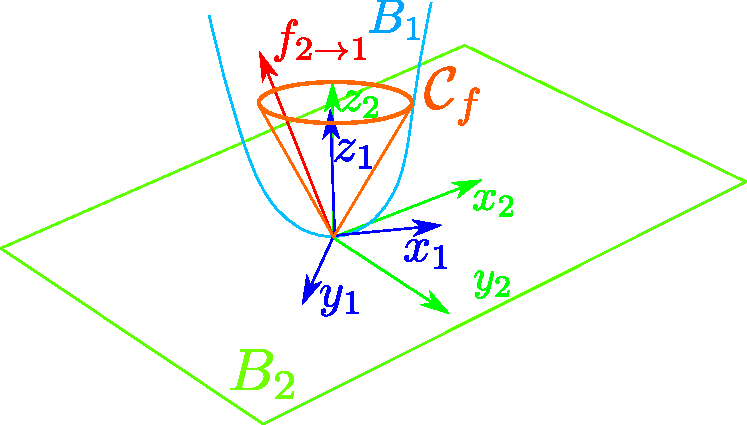
\includegraphics[width=0.6\linewidth]{frictionCone.pdf}
  \caption{Punctual unilateral Stability contact with friction}
\label{fig:frictionCone}
\end{figure}

This formulation of the interaction force defines a bilateral contact, in the sense that the force can be in any direction, $B_1$ can push as well as pull on $B_2$.

To model a unilateral contact, we must constrain the normal component of $f_{2\rightarrow 1}$ to be oriented toward the inside of $B_1$. Which means that only pushing actions can be generated, not pulling actions.
This translates into:
\begin{equation}
  \overrightarrow{f_{2\rightarrow 1}}\cdot \vec{z_1} = f_z \geq 0
\end{equation}

Furthermore, for the contact to be stable, the Coulomb friction law must be respected.
This law states that the contact force resultant must lay inside a friction cone of angle $\mu$, the friction coefficient.
Which translates into the following equation:

\begin{equation}
  \mu\|\vec{f_n}\| \geq \|\vec{f_t}\|
\end{equation}

Given the decomposition of $f_{2\rightarrow 1}$ in $F_1$, $f_{2\rightarrow 1} = f_x \vec{x_1} + f_y \vec{y_1} + f_z \vec{z_1}$.
For any punctual contact in a posture generation problem, we can add the following set of constraint to our optimization problem:

\begin{equation}
  \label{eq:unilateralContact}
  \left\{
  \begin{array}{l}
    f_z \geq 0 \\
    \mu^2 f_z^2 - f_x^2 +f_y^2 \geq 0
  \end{array}
  \right.
\end{equation}

When it comes to planar contacts on surface $S$ with $\vec{n}$ the outbound normal to $S$, the interaction force can have components of forces and moments in all directions.
The forces components intrinsic to the planar contact model are a resultant part aligned with $\vec{n}$ $\vec{f_n} = f_z \vec{z_1}$ and a moment part tangential to $S$: $\vec{m_t} = m_x \vec{x_1} + m_y \vec{y_1}$.
The forces due to friction are a tangential friction resultant part $\vec{f_t} = f_x \vec{x_1} + f_y \vec{y_1}$ and a normal friction moment $\vec{m_n} = m_z \vec{z_1}$.

This type of force can be modeled by a set of unilateral punctual efforts applied on each vertex of a polygon describing the contact area.
And ensuring that each of them lay in their respective friction cone, thus satisfying the equation~\ref{eq:unilateralContact}. As depicted in~\Figref{fig:planarContact}

\begin{figure}[htpb]
  \centering
  \setlength{\fboxsep}{0pt}%
  \setlength{\fboxrule}{1pt}%
  \fbox{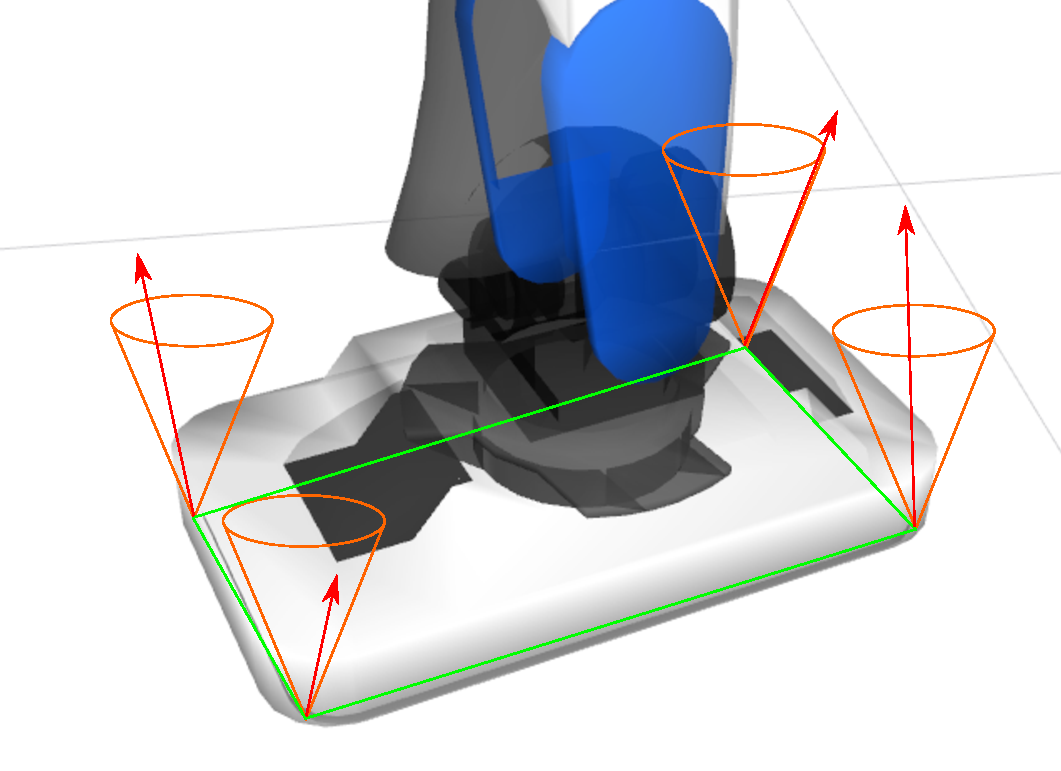
\includegraphics[width=0.6\linewidth]{planarContact.pdf}}
  \caption{Modelization of a Planar Contact between the foot on HRP4 and the ground}
\label{fig:planarContact}
\end{figure}
%}}}
%}}}
%{{{SECTION:COST FUNCTIONS
\section{Cost Functions}
\label{sec:cost_functions}

%%%%%%%%%%%%%%%%%%%%%%%%%%%%%%%%%%%%%%%%%%%%%%%%%%%%%%%%%%%%%%%%%%%%%%%
%                       SECTION COST FUNCTIONS                        %
%%%%%%%%%%%%%%%%%%%%%%%%%%%%%%%%%%%%%%%%%%%%%%%%%%%%%%%%%%%%%%%%%%%%%%%

In addition to constraints, it is often useful to add a cost function to our optimization problem.
The submanifold of feasible configurations $\mathcal{C}_F$ can contain an infinity of solutions and even some continuous solution areas in which all points are solutions.
The cost function helps to choose the `best' candidate solution.
Various types of cost functions can be chosen, for example, we can minimize the distance to a reference posture $q_R$:

\begin{equation*}
  f_\text{posture}(q) = \|q-q_R\|
\end{equation*}

The effect of that type of cost function is illustrated in~\Figref{fig:cost}. On both images, the HRP-2 Kai robot is stable, respects its joints and torques limits. The only difference is that the right one mimimizes the distance to a reference posture (standing straight with bent knees) while the left result does not use a cost function.

\begin{figure}[htpb]
  \centering
  \setlength{\fboxsep}{0pt}%
  \setlength{\fboxrule}{1pt}%
  \fbox{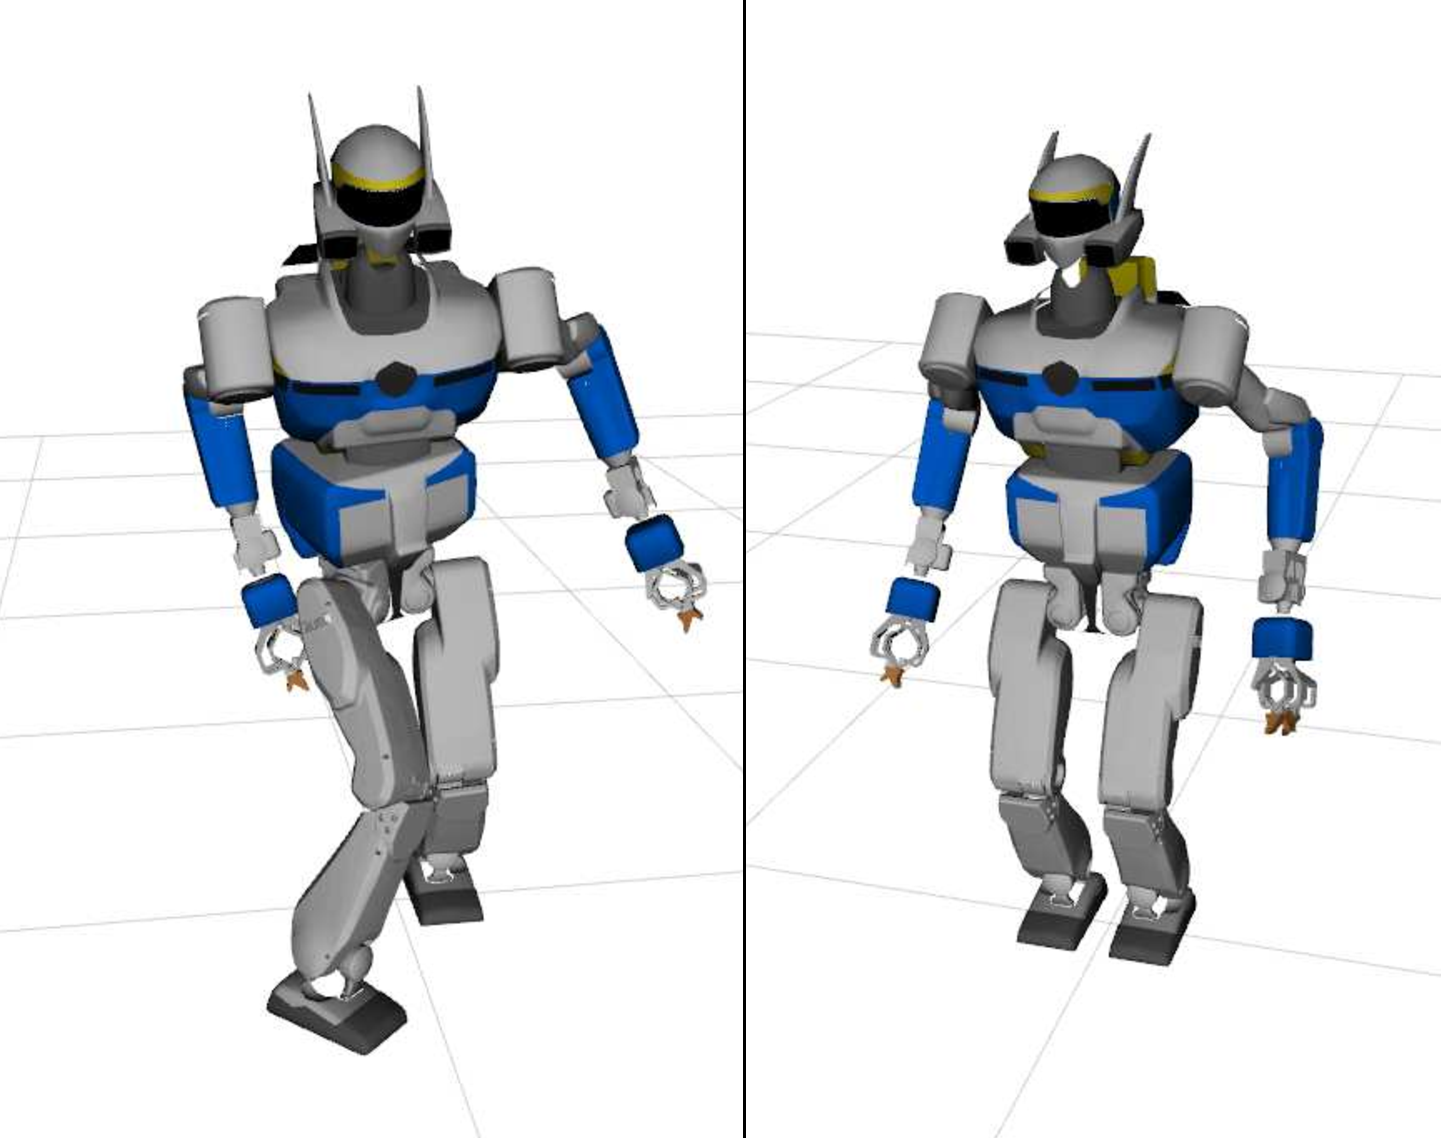
\includegraphics[width=0.5\linewidth]{cost.pdf}}
  \caption{Effect of cost function. Left: no cost function. Right: Distance to posture}
\label{fig:cost}
\end{figure}

We can also want to minimize the sum of norms of contact forces:
\begin{equation*}
  f_\text{forces}(f) = \sum\limits_i \|f_i(f)\|
\end{equation*}
Or the torques in the robot's joints:
\begin{equation*}
  f_\text{torques}(q,f) = \sum\limits_i \|\tau_i(q,f)\|
\end{equation*}
Some more custom cost functions can also be considered, for example, we can want a point $P_i$ on body $B_i$ with to be as far as possible in a direction $\vec{d}$
\begin{equation*}
  f_\text{point} (q) = -{\overrightarrow{O_W P_i}}\cdot{\vec{d}}
\end{equation*}

Any positively weighted combination of cost function can be used. In which case it is important to choose the weights carefully to scale all the costs so that they all can influence the result and none is completely dominated by another.
\begin{equation}
  f_\text{cost}(q,f) = \sum\limits_i{w_i f_i(q,f)} = w_0 f_\text{posture}(q) + w_1 f_\text{forces}(f) + w_2 f_\text{torques}(q,f) + \cdots
\end{equation}
%}}}
%{{{SECTION:CONCLUSION
\section{Conclusion}
\label{sec:Ch1_Conclusion}

%%%%%%%%%%%%%%%%%%%%%%%%%%%%%%%%%%%%%%%%%%%%%%%%%%%%%%%%%%%%%%%%%%%%%%%
%                         SECTION CONCLUSION                          %
%%%%%%%%%%%%%%%%%%%%%%%%%%%%%%%%%%%%%%%%%%%%%%%%%%%%%%%%%%%%%%%%%%%%%%%

In this section, we have seen how to formulate a robotics problem with several different tasks and objectives as an optimization problem.

We denote $\mathcal{T}_i$ the additional tasks added to the problem, which is described by the set of equations $g_i(q,f) = 0$ and inequations $h_i(q,f) \geq 0$.
The contact tasks are included in those and the equations describing them must encompass the geometric contact constraint equation like~\ref{eq:coplanarity} as well as the unilaterality and friction equations~\ref{eq:unilateralContact} in the case of a unilateral contact.

A typical robotics problem can be written as a combination of all those costs and constraints:
\begin{align}
\min_{q, f} & \quad f_\text{cost}(q,f) \nonumber\\
\text{s.t.}&
\left\{
\begin{array}{lr}
q^- \le q \le q^+\\
s(q,f) = 0 \\
\tau^- \le \tau(f,q) \le \tau^+\\
\forall \{B_i, B_j, \epsilon_{ij}\} \in Coll,\ d_{\{B_i, B_j\}}(q) > \epsilon_{ij}\\
g_i(q,f) = 0\ \ \forall\mathcal{T}_i,\\
h_i(q,f) \geq 0\ \ \forall\mathcal{T}_i.
\end{array}\right.
\label{eq:PG}
\end{align}
%}}}



%%%%%%%%%%%%%%%%%%%%%%%%%%%%%%%%%%%%%%%%%%%%%%%%%%%%%%%%%%%%%%%%%%%%%%%
%                           Second Chapter                            %
%                  Extensions of Posture Generation                   %
%%%%%%%%%%%%%%%%%%%%%%%%%%%%%%%%%%%%%%%%%%%%%%%%%%%%%%%%%%%%%%%%%%%%%%%

\chapter{Extensions of Posture Generation}
\label{cha:extensions_of_posture_generation}

\section{List of contributions}
\paragraph{Integration on Non-Inclusive Contacts in Posture Generation}

The method presented before is limiting in many cases. Ladder, stairs climbing\dots.
Sometimes it is not possible to ensure inclusion of 2 surfaces.

\begin{itemize}
  \item Contact geometry formulation
    \begin{itemize}
      \item Discretisation of contact surfaces for practical reasons
      \item Contact generation with convex surface inclusions
Usual methods for generating surface contact are based on point-to-point sampling, on rectangular inclusion, or other limiting methods. We extend that to the inclusion of convex surfaces.
      \item Inclusive contacts are no problem
      \item Non-Inclusive contacts lead to non-constant number of constraints or non-smooth gradients, cannot be solved with usual solvers with that formulation
    \end{itemize}
  \item{Non inclusive contact constraints}
    \begin{itemize}
      \item {Main Idea: Inserting an ellipse in the intersection of polygons}
      \item {Pseudo-distance(to simplify the formulation)}
      \item {Modification of the optimization problem}
      \item {Maximization of the contact area}
      \item {Using non inclusive contact to maintain stability}
      \item {Extension to singular cases}
    \end{itemize}
  \item{Simulation Results}
    \begin{itemize}
      \item{Inclined ladder climbing}
      \item{Vertical ladder climbing}
      \item{Climbing Stairs}
      \item{Walking along a path made of small objects}
    \end{itemize}
  \item{Application to ladder climbing (cf. Joris papers)}
\end{itemize}

\paragraph{On the use of lifted variables for Robotics Posture Generation}
\begin{itemize}
  \item {Introduction: "J. Albersmeyer and M. Diehl, The lifted Newton Method and its Application in Optimisation"}
  \item {Lifting Algorithm: Introduce additional variables to reduce the complexity/degree of the equations to solve. And then use a trick to re-condense the system and avoid loosing computation time}
  \item {Optimization on lifted variables}
  \item {Condensed BFGS update}
  \item {Results, experimentation}
  \begin{itemize}
    \item Symbolic Inverse Kinematics
    \item Automatic Lifting algorithm adapted to posture generation
    \item Several Solvers for lifted and non-lifted systems (Gauss Newton, SQP, lifted Newton.... )
    \item Compared many optimization methods (Globalization, regularization....)
    \item Never managed to get results faster than basic methods
  \end{itemize}
  \item{Motivation:Development of a posture generator with a specialized solver}
    \begin{itemize}
      \item Problem
        \begin{itemize}
          \item Robotics problems solved with generic solvers (IPOPT, CFSQP, fmincon...)
          \item Robotics problems(especially posture generation) are very specific (Constraints, costs, working spaces, sizes...)
        \end{itemize}
      \item Solution
        \begin{itemize}
          \item Develop a posture generator, along with a non-linear solver
          \item Better understanding of our own solver
          \item Ability to use the solver in new ways:
          \begin{itemize}
            \item Working on Manifolds
            \item Variable numbers of constraints
            \item Automatic management of variables, constraints and mathematical expressions
          \end{itemize}
        \end{itemize}
    \end{itemize}
\end{itemize}

%%%%%%%%%%%%%%%%%%%%%%%%%%%%%%%%%%%%%%%%%%%%%%%%%%%%%%%%%%%%%%%%%
%  SECTION APPLICATION TO CONTACT PLANNING ON REAL ENVIRONMENT  %
%%%%%%%%%%%%%%%%%%%%%%%%%%%%%%%%%%%%%%%%%%%%%%%%%%%%%%%%%%%%%%%%%

\section{Application to contact planning on real environment}
\subsection{Understanding the environment through a point-cloud}
Segmentation pipeline:
\begin{itemize}
  \item Acquisition
  \item Filtering
  \item Region growing segmentation
  \item Planar Extraction
  \item Planar projection and Hull convex generation
  \item Re-orientation and transfer to the planner
\end{itemize}

\subsection{Contact generation with convex surface inclusions}
Usual methods for generating surface contact are based on point-to-point sampling, on rectangular inclusion, or other limiting methods. We proposed to extend that to the inclusion of convex surfaces.

\subsection{Simulated scenarios planned on real-environment}
We present 2 planned scenarios with the HRP-2 robot



%%%%%%%%%%%%%%%%%%%%%%%%%%%%%%%%%%%%%%%%%%%%%%%%%%%%%%%%%%%%%%%%%%%%%%%%%
%  SECTION INTEGRATION ON NON-INCLUSIVE CONTACTS IN POSTURE GENERATION  %
%%%%%%%%%%%%%%%%%%%%%%%%%%%%%%%%%%%%%%%%%%%%%%%%%%%%%%%%%%%%%%%%%%%%%%%%%

\section{Integration on Non-Inclusive Contacts in Posture Generation}

The method presented before is still limiting in many cases. Ladder, stairs climbing\dots.
Sometimes it is not possible to ensure inclusion of 2 surfaces.

\subsection{Contact geometry formulation}
\label{sec:background}
Present the difficulties related to intersecting 2 convex polygons. Non-constant number of constraints.
Usual solution: patching

\subsection{Non inclusive contact constraints}
\subsubsection{Main Idea}
\subsubsection{Pseudo-distance}
\subsubsection{Modification of the optimization problem}
\subsubsection{Maximixation of the contact area}
\subsubsection{Using non inclusuve contact to maintain stability}
\subsubsection{Extension to singular cases}
\subsection{Simulation Results}
\subsubsection{Inclined ladder climbing}
\subsubsection{Vertical ladder climbing}
\subsubsection{Climbing Stairs}
\subsubsection{Walking along a path made of small objects}

%%%%%%%%%%%%%%%%%%%%%%%%%%%%%%%%%%%%%%%%%%%%%%%%%%%%%%%%%%%%%%%%%%%%
%  ON THE USE OF LIFTED VARIABLES FOR ROBOTICS POSTURE GENERATION  %
%%%%%%%%%%%%%%%%%%%%%%%%%%%%%%%%%%%%%%%%%%%%%%%%%%%%%%%%%%%%%%%%%%%%

\section{On the use of lifted variables for Robotics Posture Generation}
\label{sec:liftedVariables}

\subsection{Introduction}
\label{subsec:Introduction}

\subsection{Lifting Algorithm}
\label{subsec:LiftingAlgorithm}

\subsection{Optimization on lifted variables}
\label{subsec:Optimization on lifted variables}

\subsection{Condensed BFGS update}
\label{subsec:Condensed BFGS update}

\subsection{Results, experimentation}
\label{subsec:Results}

\subsection{conclusion}
\label{subsec:conclusion}

%%%%%%%%%%%%%%%%%%%%%%%%
%  SECTION CONCLUSION  %
%%%%%%%%%%%%%%%%%%%%%%%%

\section{Discussion and conclusion}
All that is very nice, but still many limitations and possible improvements.
Transition to Posture generation on Non-Euclidean Manifolds.





%%%%%%%%%%%%%%%%%%%%%%%%%%%%%%%%%%%%%%%%%%%%%%%%%%%%%%%%%%%%%%%%%%%%%%%
%                            Third Chapter                            %
%               Optimization on non-Euclidean Manifolds               %
%%%%%%%%%%%%%%%%%%%%%%%%%%%%%%%%%%%%%%%%%%%%%%%%%%%%%%%%%%%%%%%%%%%%%%%

\chapter{Optimization on non-Euclidean Manifolds}
\label{chapter:optimization_on_noneuclidean_manifolds}

\nomenclature[x-M]{$\mathcal{M}$}{A manifold}
\nomenclature[x-TxM]{$T_x\mathcal{M}$}{The tangent space to $\mathcal{M}$ at point $x$}

\graphicspath{{Chapter3-Manifolds/Figs/}{Chapter3-Manifolds/Figs/Humanoids2015/}}

%{{{ LIST OF CONTRIBUTIONS
%\section{List of contributions}
%\begin{itemize}
  %\item{Optimisation on Manifolds}
    %\begin{itemize}
      %\item Definition and examples of non-Euclidean manifolds
        %\begin{itemize}
          %\item $\mathbb{R}^n$
          %\item $SO(3)$
          %\item $S2$
          %\item Cartesian Products
        %\end{itemize}
      %\item Representation space vs Tangent space vs manifold
      %\item Local parametrization, notion of retractation
      %\item Computation of function's derivatives, differentiation of retractation
      %\item Hessian update on manifolds, notion of vector transport and application to BFGS and SR1 updates
      %\item Computation of distances, notion of logarithm
    %\end{itemize}
  %\item{Practical Implementation: PGSolver}
    %\begin{itemize}
      %\item General SQP algorithm adapted to local parametrization of manifolds.
      %\item Local QP and resolution with LSSOL
      %\item Feasibility problems and resolution with LSSOL
      %\item Acceptance criterion:
        %\begin{itemize}
          %\item Merit function
          %\item Filter
        %\end{itemize}
      %\item Globalization method:
        %\begin{itemize}
          %\item Line-Search
          %\item Trust-Region
            %\begin{itemize}
              %\item Notions of limit-Map vs trust-region vs problem's boundaries
              %\item Decisions of increase or decrease of trust region's size
              %\item Anisotrope trust-region
            %\end{itemize}
        %\end{itemize}
      %\item Hessian Update:
        %\begin{itemize}
          %\item BFGS
          %\item SR1
          %\item Fletcher LQNU
          %\item Individual vs grouped updates
          %\item Limited memory updates
        %\end{itemize}
      %\item Termination conditions:
        %\begin{itemize}
          %\item Satisfaction of KKT constraints
          %\item Null step
          %\item Failure of QP, FP, other\dots
        %\end{itemize}
      %\item Restoration Phase:
        %\begin{itemize}
          %\item Problem to solve: minimization of violation, relaxation of violated cstr
          %\item Exit condition: Feasible problem
          %\item Second-order correction phase
        %\end{itemize}
    %\end{itemize}
  %\item{Applications and testings of PGSolver on non-robotic problems}
    %\begin{itemize}
      %\item Point cloud fitting
      %\item Surface parametrisation
      %\item Cube stacks
      %\item Schitkowsky
    %\end{itemize}
%\end{itemize}
%}}}

%{{{ INTRODUCTION TO OPTIMIZATION ON MANIFOLDS
\section{Introduction to optimization on Manifolds}
\label{sec:introduction_to_optimization_on_manifolds}

Posture generation has been formulated as a problem over a Euclidean space.
Robots variable may however be more naturally expressed over non-Euclidean manifolds.
The archetypes for this are the rotation part of the root body of a humanoid robot, and ball joints, whose variables live in $SO(3)$.
Some typical tasks are also naturally formulated on different manifolds.
For example, for making contact with any object that can be mapped on a sphere, the contact point position for this object can be parametrized in $S2$~\cite{escande:icra:2016}.
Human shoulder can be elegantly parametrized on $S2\times\mathbb{R}$, as proposed in~\cite{baerlocher}.

Formulating the problem over $\mathbb{R}^n$ leads either to discontinuities that can prevent the convergence of the optimization solver, or to cumbersome writing to specify that the variable is actually living on a manifold (see~\cite{bouyarmane:humanoids:2012}).

For example, let us consider an optimization problem over the $SO(3)$ manifold:

\begin{align}
\label{eq:pb_on_SO3}
  \minimize_{x \in SO(3)} & \quad f(x)\\
  \text{subject to}&
  \begin{array}{lr}
    l \leq c(x) \leq u \nonumber
  \end{array}
\end{align}

$SO(3)$ is a 3-dimensional manifold.
As such, it can be parametrized \emph{locally} by $3$ variables, for example, a choice of Euler angles, but any such parametrization necessarily exhibits singularities when taken as a global map (e.g.\ gimbal lock for Euler angles), which can be detrimental to our optimization process.

For this reason, when addressing $SO(3)$ with classical optimization algorithms, it is often preferred to use one of the two following parametrizations:
\begin{itemize}
    \item unit quaternion, \emph{i.e.} an element $q$ of $\mathbb{R}^4$ with the additional constraint $\left\|q\right\| = 1$,
    \item rotation matrix, \emph{i.e.} an element $R$ of $\mathbb{R}^{3 \times 3}$ (or equivalently $\mathbb{R}^9$) with the additional constraints $R^T R = I$ and $\det{R} \geq 0$.
\end{itemize}

Then, if we use the unit quaternion parametrization, the problem~\ref{eq:pb_on_SO3} becomes:
\begin{align}
\label{eq:pb_on_SO3_quaternion}
  \minimize_{q \in \mathbb{R}^4} & \quad f(q)\\
  \text{subject to}&
  \left\{\begin{array}{lr}
    {l} \leq c(q) \leq {u} \nonumber\\
    \|q\| - 1 = 0
  \end{array}\right.
\end{align}

The problem to solve has 4 dimensions (to represent a 3-dimensional manifold), and has an additional constraint that is entirely due to our formulation choice.
With this formulation, it is guaranteed that the solution $q^*$ is a unit quaternion, but not that all the iterates $q_k$ along the optimization process have a unit norm.
During the optimization process, at each iteration, an increment $\delta$ is computed by solving a quadratic problem that approximates~\ref{eq:pb_on_SO3_quaternion} locally around $q_k$.
In particular, this quadratic problem approximates the constraints linearly, thus, for any step $\delta$ not null, from a unit-norm quaternion iterate $q_k$, the next iterate $q_{k+1} = q_k + \delta$ does not respect the unit-norm constraint (it respects the \emph{linearization} of the unit-norm constraint).
So the quaternion $q_{k+1}$ does not represent a rotation.
Some additional treatment needs to be implemented.
For example, normalizing the quaternion at each iteration, then it represents a rotation, but this normalization must be taken into account in the constraints, cost functions, and their differentiations, which is an additional programming burden.
Similar issues can be found with the $\mathbb{R}^{3\times 3}$ matrix representation.

The alternative is to use optimization software working natively with manifolds~\cite{brossette:Humanoids:2015}\cite{absil:book:2008} and solve the optimization problem as it is written in~\ref{eq:pb_on_SO3}.
It has an immediate advantage: we can write directly the problem without the need to add any parametrization-related constraints.
Working directly with manifolds also has the advantage that at each iteration, the variables of the problem represent an element of the manifold.
This is not the case with the other formulations we discussed, as the (additional) constraints are guaranteed to be satisfied only at the end of the optimization process.
Having intermediate values naturally staying on the manifold can be useful to evaluate additional functions that pre-suppose it (additional constraints, external monitoring $\ldots$).
It can also be leveraged for real-time applications where only a short time is allocated repeatedly to the optimization, so that when the optimization process is stopped after a few iterations, the output is valid in the sense that it is always a point of the manifold.

With non-manifold formulations, at any given iteration, the parametrization-related constraints can be violated, thus, the variables might not lie in the manifold.
It is then needed to project them on it.
Denoting $\pi$ the projection (for example $\pi = \frac{q}{\left\|q\right\|}$ in the unit quaternion formulation), to evaluate a function $f$ on a manifold, we need to compute $f \circ \pi$.
If further the gradient is needed, that projection must also be accounted for (authors in~\cite{bouyarmane:humanoids:2012} explain that issue in great details for robotics problems with free-floating bases).

In this chapter, we present a new nonlinear constrained optimization solver able to work on generic smooth manifolds.
We take inspiration from the approach used for unconstrained optimization on manifold~\cite{absil:book:2008} and adapt it to constrained optimization.
To the best of our knowledge, constrained optimization on manifold has drawn few research for now.
This is likely due to the fact that in most problems the only constraint is to be on the manifold, in that case, unconstrained optimization on manifold is enough.
We are only aware of the work of Schulman \emph{et al.}~\cite{Schulman2014}, where the authors explain the adaptation of their solver to work on $SE(3)$.
This adaptation is however not valid for general manifolds without more care about hessian computation.

A background motivation for this work is to have our own optimization solver, instead of a black box.
We will now be able to specialize the solver for robotic problems, by leveraging modeling properties and approximations, for a gain in time and robustness.
%We also look forward to using this solver for problems with a varying number of constraints along the iterations (such as when complex collision constraints are considered).

%}}}
%{{{ OPTIMIZATION ON MANIFOLDS
\section{Optimization on Manifolds}
\label{sec:optimization_on_manifolds}

In this section, we describe a Sequential Quadratic Programming (SQP) approach~\cite{nocedal:book:2006} to solve the following non-linear constrained optimization program

\begin{align}
\label{eq:optim_problem}
  \minimize_{x \in \mathcal{M}} & \quad f(x)\\
  \text{subject to}&
  \begin{array}{lr}
    l \leq c(x) \leq u \nonumber
  \end{array}
\end{align}

where $\mathcal{M}$ is a $n$-dimensional smooth manifold and $c$ is a $m$-dimensional real-valued function.

%{{{ REPRESENTATION PROBLEM
\subsection{Representation problem}
When $\mathcal{M} = \mathbb{R}^n$, the problem~(\ref{eq:optim_problem}) is solved iteratively, starting from an initial guess $x_0$ and performing successive steps $x_{i+1} = x_i + {\bf p_i}$ where ${\bf p_i}$ is the increment found at the $i$-th iteration, until convergence is achieved.
The strategy to compute ${\bf p_i}$ depends on the solver.

This classical scheme cannot be readily applied to optimization over non-Euclidean manifolds.
First of all, only (a subset of) the real numbers can be stored in computers.
To manipulate elements of $\mathcal{M}$ we need to choose a way to represent them in memory.
This boils down to choosing a representation space $\mathbb{E} = \mathbb{R}^r$ (with $r \geq n$) and a map
\begin{equation}
  \psi\ :\
  \begin{array}{ccc}
    x & \reduce{\mapsto}{6} & \mathbf{x} \\
    \mathcal{M} & \reduce{\rightarrow}{6} & \mathbb{E}
  \end{array}\nonumber%
\end{equation}
In the following, we identify $\mathcal{M}$ with the set $\psi(\mathcal{M}) \subseteq \mathbb{E}$.

With this representation, it is tempting to simply transform problem~(\ref{eq:optim_problem}) as an optimization over $\mathbb{R}^r$ with objective $f \circ \psi^{-1}$ and constraint $c \circ \psi^{-1}$, and solve it with a usual solver.
But depending on the representation choice, one of the two following problems arises:\\
(i) $r=n$, then it is not possible in the general non-Euclidean case to find $\psi$ without derivative discontinuities.
This can lead to critical convergence problems, \\
(ii) $r>n$, then most elements of $\mathbb{E}$ do not represent an element of $\mathcal{M}$ %($\psi(\mathcal{M})$ is a measure-zero subset of $\mathbb{E}$)
and $\psi$ cannot be surjective.
Constraints need to be added to force the solution on $\mathcal{M}$.
As a result, the problem has more variables and constraints w.r.t (i).
Moreover, the additional constraints are unlikely to be met along the iteration process (even if $x_i$ is an element of $\mathcal{M}$, $x_i+{\bf p_i}$ is likely not, as nothing enforces it).
This means that in order to evaluate $f \circ \psi^{-1}$ and $c \circ \psi^{-1}$ at a given $x_i$, one has to project it on $\psi(\mathcal{M})$ first, effectively computing $f \circ \psi^{-1} \circ \pi$ and $c \circ \psi^{-1} \circ \pi$, where $\pi$ is the projection.
The composition by $\pi$ is an additional burden in programming (see e.g.\ in~\cite{bouyarmane:humanoids:2012a}).
Figure~\ref{fig:stepOnSphere} illustrates the difference between a step through $\varphi$ in optimization on manifolds and a step followed by a projection as is done in classical optimization.

\begin{figure}[htpb]
  \centering
  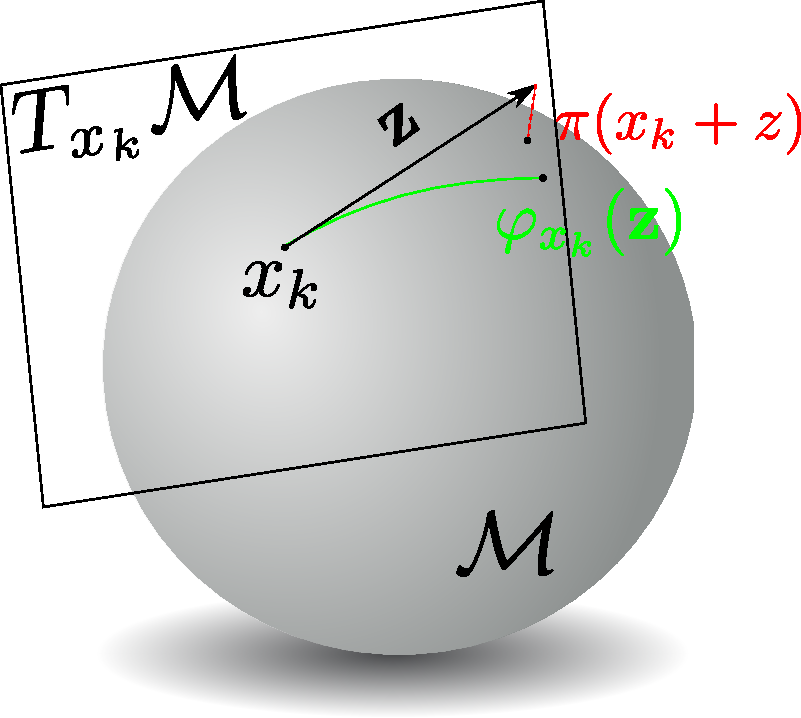
\includegraphics[width=0.5\linewidth]{Humanoids2015/stepOnSphere.pdf}
  \caption{StepOnSphere}
\label{fig:stepOnSphere}
\end{figure}

As a simple example, the set of 3D-rotations $SO(3)$ is a manifold of dimension $3$.
The following (classical) choices can be made
\begin{itemize}
  \item Rotation matrix ${\bf R} \in \mathbb{R}^{3\times 3} \approx \mathbb{R}^9$, additional constraints: $\{{\bf R}^t{\bf R} = I\ ,\ \det({\bf R})=1\}$, projection by orthogonalization,
  \item Quaternion ${\bf q} \in \mathbb{R}^4$, additional constraints: $\{ \left\|{\bf q}\right\|=1\}$, projection $\pi({\bf x}) = {\bf x}/\left\|{\bf x}\right\|$,
  \item Euler angles ($\mathbb{E} = \mathbb{R}^3$), singularities when reaching gimbal lock.
\end{itemize}

%}}}
%{{{ LOCAL PARAMETRIZATION
\subsection{Local parametrization}
By definition, there is always, at a point $x$ of a smooth $n$-dimensional manifold $\mathcal{M}$, a smooth map $\varphi_x$ between an open set of $T_x\mathcal{M}\approx \mathbb{R}^n$, the tangent space to $\mathcal{M}$ at $x$, and a neighborhood of $x$ in $\mathcal{M}$, with $\varphi_x(0) = x$.

\begin{equation}
  \varphi_x\ :\
  \begin{array}{ccc}
    \mathbf{z} & \reduce{\mapsto}{6} & \varphi_x(\mathbf{z}) \\
    T_x\mathcal{M} & \reduce{\rightarrow}{6} & \mathcal{M}
  \end{array} \nonumber%
\end{equation}

$T_x\mathcal{M}$ can be identified with $\mathbb{R}^n$, but in some cases, it needs to be considered as a hyperplan of a higher dimensionality space.
For example in figures~\ref{fig:stepOnSphere} and~\ref{fig:phimap}, $T_x\mathcal{M}$ is a 2-dimensional hyperplan embedded in $\mathbb{R}^3$.
We denote $T_x\mathbb{E}$ the representation space of $T_x\mathcal{M}$.
This gives us a local parametrization for $\mathcal{M}$.
The driving idea of the optimization on manifolds is to change the parametrization at each iteration.
Applying this idea, we can reformulate Problem~(\ref{eq:optim_problem}) around $x_i$ as
\begin{align}
\label{eq:local_problem}
\minimize_{{\bf z} \in T_{x_i}\mathcal{M}} & \quad f \circ \varphi_{x_i}({\bf z}) \\
  \text{subject to}&
  \begin{array}{rcl}
    {l} \leq & \reduce{c \circ \varphi_{x_i}({\bf z})}{8}& \leq {b} \nonumber
  \end{array}
\end{align}
This is an optimization problem on $\mathbb{R}^n$.
If we perform one iteration of a classical solver starting from ${\bf z_0} = 0$, we get an iterate ${\bf z_1}$, which corresponds to the iterate $x_{i+1} = \varphi_{x_i}({\bf z_1})$.
We can then reformulate Problem~(\ref{eq:optim_problem}) around $x_{i+1}$, perform a new iteration and repeat the process until convergence.

\begin{figure}[!htb]
  \centering
  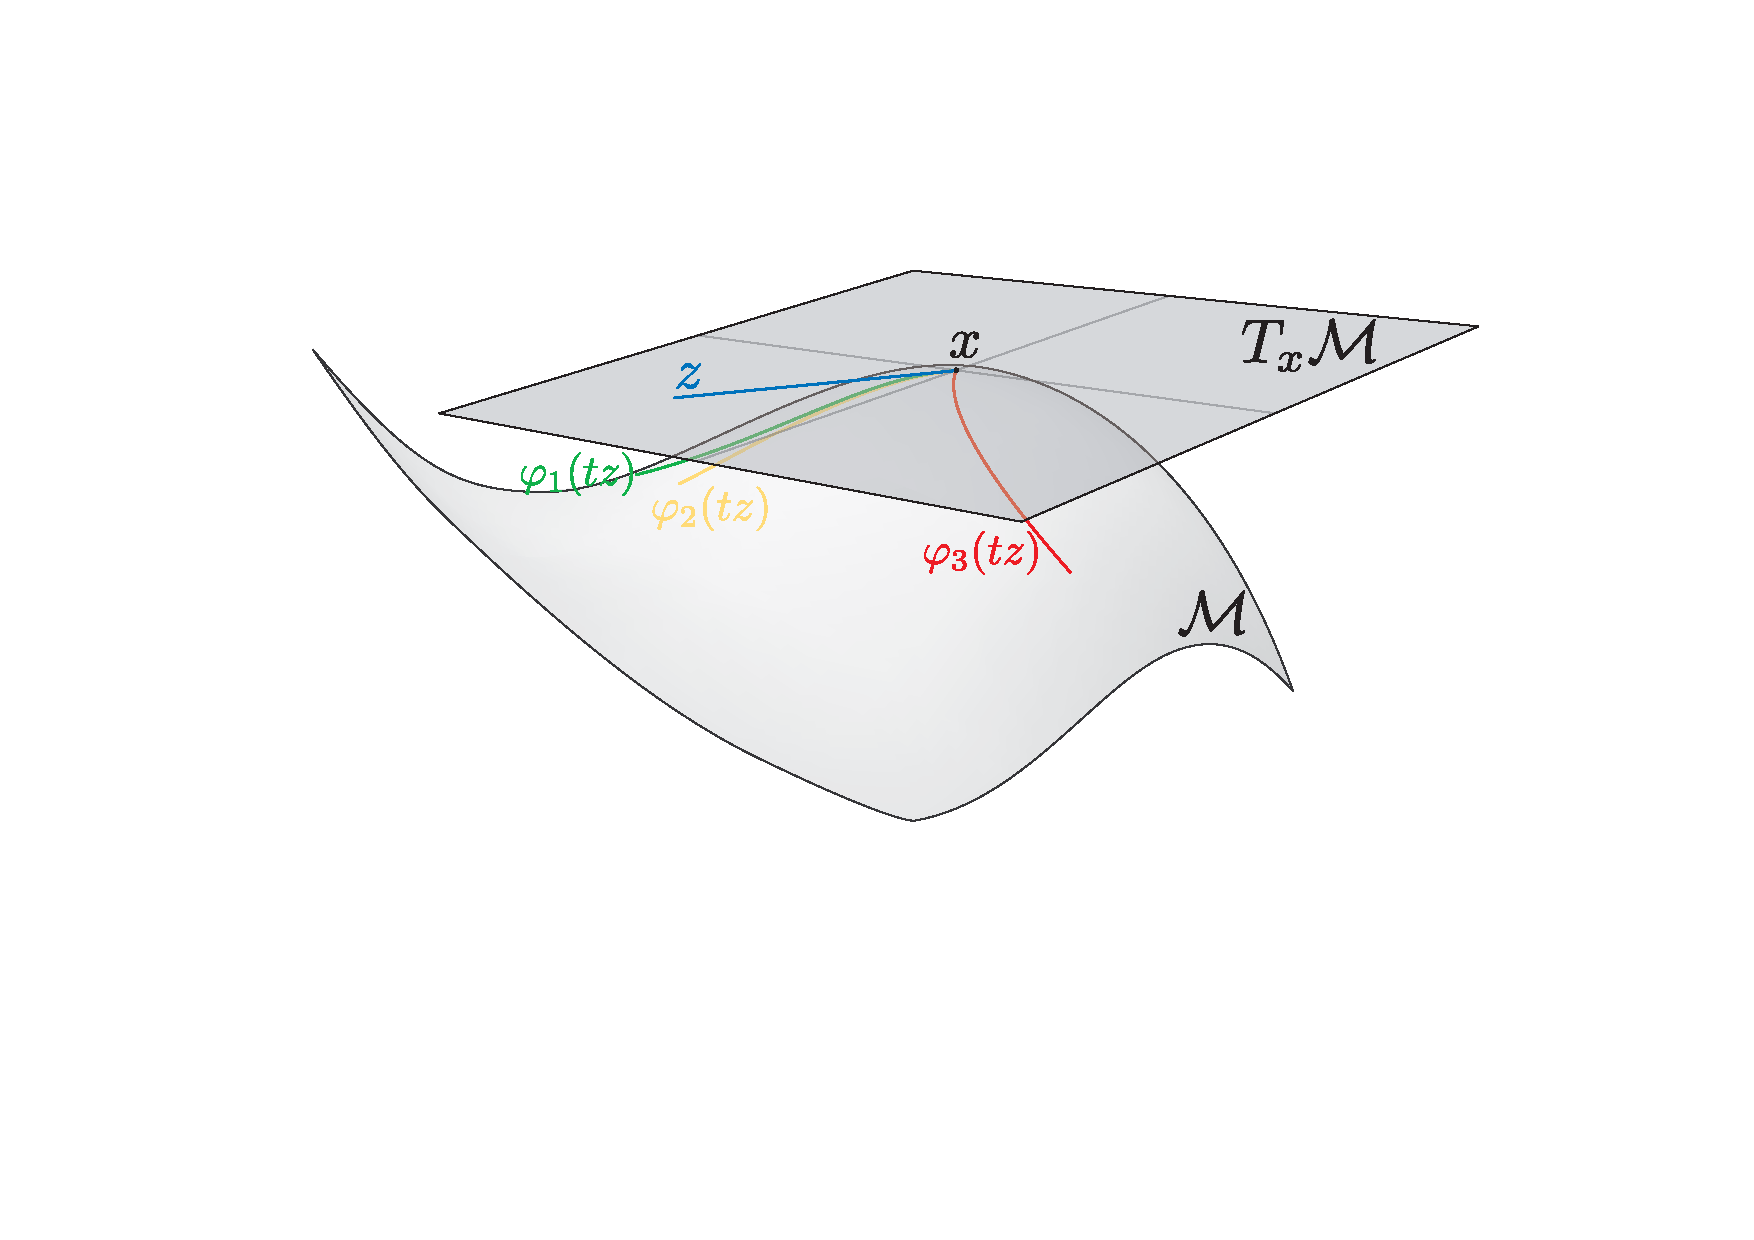
\includegraphics[width=.9\linewidth]{Humanoids2015/manifold.pdf}
  \caption{There are many possible choices for $\varphi_{x}$ but not all yield a curve $\varphi_{x}(t{\bf z})$ which is going in the same direction as ${\bf z}$: $\varphi_{1}$ and $\varphi_{2}$ are correct choices, $\varphi_{3}$ is not.}
\label{fig:phimap}
\end{figure}

However, convergence cannot be achieved without care on the choice of $\varphi_{x_i}$: it must be such that for any ${\bf z}$, the curve $t \mapsto \varphi_{x_i}(tz)$ is tangent to ${\bf z}$, see Fig.~\ref{fig:phimap}, so that the update $x_{i+1} = \varphi_{x_i}({\bf z_1})$ is made in the direction given by ${\bf z_1}$.

The exponential map is a good theoretical candidate, but it is often impractical or expensive to compute.
Depending on the manifold, cheaper maps can be chosen.

With the iterative formulation approach described above, we do not have any parametrization issue, do not need additional constraints, and have the minimum number of optimization parameters.
But we still need a map $\psi$ and real space $\mathbb{E}$ to represent the $x_i$ and keep track of them in a global way.
The ${\bf x_i}$ are guaranteed to be on $\mathcal{M}$ so we can choose a representation with $r>n$ where $\psi$ is singularity-free without any drawback.
Also, the programmer can write the function $f' = f \circ \psi^{-1}$ as if it was a function from $\mathbb{E}$ to $\mathbb{R}$ without the need to project on $\psi(\mathcal{M})$ first (same goes for $c' = c \circ \psi^{-1}$).
For example if $\mathcal{M} = SO(3)$ and $\mathbb{E} = \mathbb{R}^{3\times 3}$, ${\bf x_i}$ is automatically a rotation matrix and can be used directly as such when writing the function.

%}}}
%{{{ LOCAL SQP ON MANIFOLDS
\subsection{Local SQP on manifolds}
\label{local_sqp_on_manifolds}
We choose to adopt an SQP approach to solve our problem.
We first define the Lagrangian function
\begin{equation}
  \mathcal{L}_x ({\bf z}, \lambda) = f\circ \varphi_x({\bf z}) - \lambda^T c \circ \varphi_x({\bf z})
\end{equation}
with $\lambda \in \mathbb{R}^m$ the vector of Lagrange multipliers, and note $H_k$ the Hessian matrix $\nabla_{zz}^2 \mathcal{L}_{x_k}$.
Taking ${\bf z_0} = 0$, the $k$-th SQP step for Problem~(\ref{eq:local_problem}) is computed by solving the following quadratic program:

\begin{align}
  \label{eq:SQPStep}
  \minimize_{\bf z \in \mathbb{R}^n } & \quad {\frac{\partial f\circ \varphi_{x_k}}{\partial {\bf z}}(0)}^T {\bf z } + \frac{1}{2} {\bf z }^T H_k{\bf z }\\
  \text{subject to}&
  \begin{array}{lr}
    \text{l} \leq c\circ \varphi_{x_k}(0) + \frac{\partial c\circ \varphi_{x_k}}{\partial {\bf z}}(0) {\bf z }\leq \text{u}\\
  \end{array} \nonumber%
\end{align}

The basic SQP approach adapted to manifolds can be summarized as follows
\begin{enumerate}
  \item set $k=0$ and $x_k$ to the initial value
  \item compute ${\bf z}$ from Problem~(\ref{eq:SQPStep}) for current $x_k$
  \item set $x_k = \varphi_{x_k}({\bf z})$
  \item if convergence is not yet achieved go-to step 2
\end{enumerate}

Computations of function values and derivatives are based on the fact that $f \circ \varphi = f' \circ \psi \circ \varphi$ (and same for $c$), and
\begin{align}
  f'\ :\
  \begin{array}{ccc}
    \mathbb{E} & \reduce{\rightarrow}{6} & \mathbb{R}
  \end{array} \nonumber\\
  \psi\circ\varphi:
  \begin{array}{ccc}
    \mathbb{R}^n & \reduce{\rightarrow}{6} & \mathbb{E}
  \end{array} \nonumber%
\end{align}
are representable functions (whereas $f$, $\psi$ and $\varphi_x$ are not, due to the fact that they feature $\mathcal{M}$ as input or output).
The gradient of $f \circ \varphi_x$ is
\begin{align}
  \frac{\partial f\circ\varphi_x}{\partial {\bf z}}=
  \frac{\partial f'}{\partial y}(\psi\circ\varphi_x)\times
  \frac{\partial (\psi\circ\varphi_x)}{\partial {\bf z}}
\end{align}

$\frac{\partial f'}{\partial y}$ denotes the gradient of $f'$ with respect to an element of $\mathbb{E}$, which is the derivative that is usually calculated for use in classical optimization schemes.

%}}}
%{{{ DESCRIPTION OF NON-EUCLIDEAN MANIFOLDS
\subsection{Description of non-Euclidean manifolds}
\label{sub:examples_on_non_euclidean_manifolds}

For each elementary manifold $\mathcal{M}$, we need to define a set of elements and operations.
Those need only to be implemented once for each elementary manifold (it is then trivial to get those functions for Cartesian products of manifolds).
The composition with $f'$ and $c'$ is done automatically.
The expression of those functions is adapted from~\cite{boumal:jmlr:2014}.

\paragraph{Retractation:}
We need a retractation operation $\psi\circ\varphi_x$ (that we denote simply $\varphi_x$) and its derivative.
During the optimization process, we need the expression of the derivatives of $\varphi_x$ in order to compute the gradients of the cost function and constraints at the beginning of each iteration to later compute the approximated quadratic problem to be solved in that iteration.
Because we change the parametrization of our problem to be centered on $x_k$ at each iteration, we only ever need to evaluate the gradient of $\varphi_x$ for $\mathbf{z}=0$, $\frac{\partial \varphi_x}{\partial \mathbf{z}}(0)$.
In many cases, this quantity is invariant w.r.t $x$ and can be computed once and for all for each manifold.

\paragraph{Pseudo-Logarithm and distances:}
It is necessary to be able to compute distances on manifolds.
For that, we define the pseudo-logarithm (aka pseudolog), which is the inverse of the retractation operator.
Note that the logarithm map is the inverse of the exponential map.
\begin{equation*}
  \zeta_x:\mathcal{M}\rightarrow T_x\mathcal{M}
\end{equation*}
\begin{equation*}
  \forall (x,y)\in \mathcal{M}\times\mathcal{M},\ \mathbf{z}:=\zeta_x(y)\ \text{is such that}\ \varphi_x(\mathbf{z}) = y
\end{equation*}
The pseudolog operator gives the vector of $T_x\mathcal{M}$ to go from $x$ to $y$.
It is used to compute the (pseudo-) distance between two points of $\mathcal{M}$
\begin{equation*}
  \dist(x,y) = \|\zeta_x(y)\|
\end{equation*}

\paragraph{Vector Transport:}
To compare two vectors $\mathbf{v}_1$ and $\mathbf{v}_2$ defined in tangent spaces of different points, respectively, $T_{x_1}\mathcal{M}$ and $T_{x_2}\mathcal{M}$, it is necessary to transport $\mathbf{v}_1$ into $T_{x_2}\mathcal{M}$.
Figure~\ref{fig:transport} illustrates the transport of a vector $\mathbf{v}_1$ from $T_{x_1}\mathcal{M}$ to $T_{x_2}\mathcal{M}$.
$\mathbf{v}_2$ can then be compared to the transported $\mathbf{v}_1$: $\mathcal{T}_{x_1,\mathbf{z}}(\mathbf{v}_1)$.
This operation will come in handy for the computation of Hessian approximations explained later in this chapter.

\begin{figure}[htpb]
  \centering
  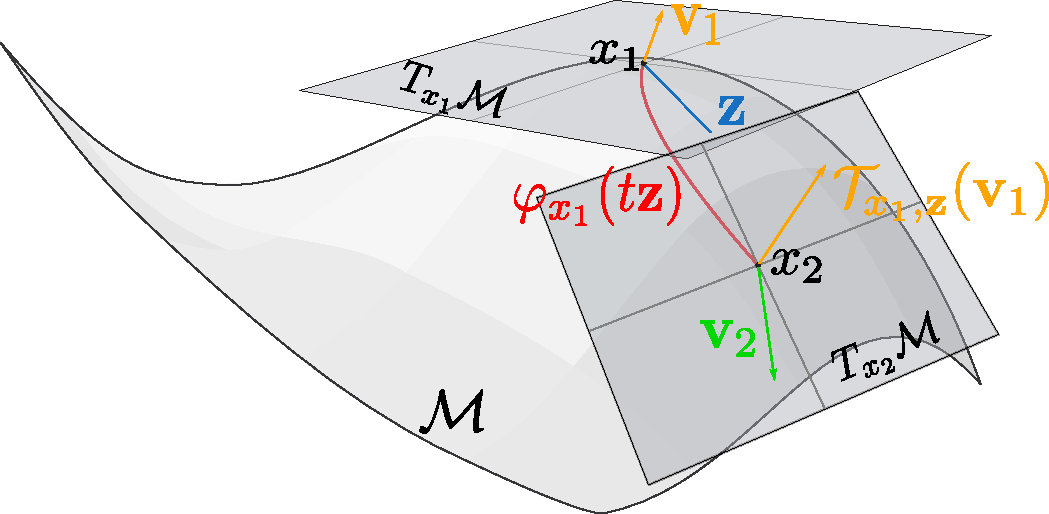
\includegraphics[width=0.8\linewidth]{transport.pdf}
  \caption{Vector transport on a non-Euclidean manifold}
\label{fig:transport}
\end{figure}

%\paragraph{Projections:} A projection operator on $\mathcal{M}$, as well as one on $T_x\mathcal{M}$ can come in handy, especially to help eliminate some numerical errors when necessary.

\paragraph{Limits on tangent map:} The tangent map can present some singularities, thus it is necessary to limit the length of steps made through retractation to the validity region of each manifold.

To summarize, for each elementary manifold $\mathcal{M}$, we need to implement the following elements:
\begin{itemize}
  \item Tangent Space at point $x$, $T_x\mathcal{M}$
  \item Embedding spaces $\mathbb{E}$ and $T_x\mathcal{M}$
  \item Retractation operator $\varphi:\ (x,\mathbf{z}) \rightarrow \varphi_x(\mathbf{z})$
  \item Gradient of the retractation operator $\partial \varphi(x):\rightarrow \frac{\partial \varphi_x}{\partial \mathbf{z}}(0)$
  \item Pseudo-logarithm operator $\zeta:\ (x,y) \rightarrow \zeta_x(y)$
  \item Gradient of pseudo-logarithm operator $\frac{\partial \zeta_x}{\partial y}(y)$
  \item Transport operator $\mathcal{T}:\ (x,\mathbf{z}, \mathbf{v})\rightarrow \mathcal{T}_{x,\mathbf{z}}(v)$
  \item Projection from $\mathbb{E}$ on $\mathcal{M}$, $\pi_\mathcal{M}$
  \item Projection from $T_x\mathbb{E}$ on $T_x\mathcal{M}$, $\pi_{T_x\mathcal{M}}$
  \item Limits of the tangent map, $\lim$
\end{itemize}

%{{{ THE REAL SPACE MANIFOLD $\MATHBB{R^N$}
\subsubsection{The Real Space manifold $\mathbb{R}^n$}
\label{ssub:the_real_space}
Since $\mathbb{R}^n$ is a Euclidean manifold, the operations that we use on it are straightforward.

\begin{table} [H]
\caption{Description of the $\mathbb{R}^n$ manifold}
\centering
\begin{tabular}{cc}
  \toprule
  $\mathcal{M}$ & $\mathbb{R}^n$ \\
  \midrule
  $\mathbb{E}$ & $\mathbb{R}^n$ \\
  \midrule
  $T_x\mathcal{M}$ & $\mathbb{R}^n$ \\
  \midrule
  $T_x\mathbb{E}$ & $\mathbb{R}^n$ \\
  \midrule
  $\varphi_x(\mathbf{z})$ & $\mathbf{x} + \mathbf{z}$ \\
  \midrule
  $\partial \varphi_x(0)$ & $\mathbb{I}_n$ \\
  \bottomrule
\end{tabular}
\quad
\begin{tabular}{cc}
  \toprule
  $\zeta(x,y)$ & $\mathbf{y} - \mathbf{x}$ \\
  \midrule
  $\frac{\partial \zeta_x}{\partial y}(x)$ & $\mathbb{I}_n$ \\
  \midrule
  $\mathcal{T}(x,\mathbf{z}, \mathbf{v})$ & $\mathbf{v}$ \\
  \midrule
  $\pi_\mathcal{M}(\mathbf{x})$ & $\mathbf{x}$ \\
  \midrule
  $\pi_{T_x\mathcal{M}}(\mathbf{z})$ & $\mathbf{z}$ \\
  \midrule
  $\lim$ & $\|\mathbf{v}\| \leq \infty$ \\
  \bottomrule
\end{tabular}
\end{table}
%}}}
%{{{ THE 3D ROTATION MANIFOLD SO(3): MATRIX REPRESENTATION
\subsubsection{The 3D Rotation manifold $\mathbf{SO(3)}$: Matrix representation}
\label{ssub:the_3d_rotation_manifold_matrix_representation}

An element $x$ of $SO(3)$ is represented by $\mathbf{x}=\psi(x)$ in $\mathbb{R}^{3\times 3}$ by:
\begin{equation}
  x\in SO(3),\ \mathbf{x} =\begin{bmatrix}
    x_{00} & x_{01} & x_{02} \\
    x_{10} & x_{11} & x_{12} \\
    x_{20} & x_{21} & x_{22} \\
  \end{bmatrix}
\end{equation}

We recall the operators
\begin{equation}
\widehat{.}: \begin{bmatrix}
  \omega_0\\\omega_1\\\omega_2\\
\end{bmatrix}
\rightarrow
\begin{bmatrix}
  0 & -\omega_2 & \omega_1 \\
  \omega_2 & 0 & -\omega_0 \\
  -\omega_1 & \omega_0 & 0\\
\end{bmatrix}
\end{equation}
And its inverse:
\begin{equation}
\widecheck{.}: \begin{bmatrix}
    x_{00} & x_{01} & x_{02} \\
    x_{10} & x_{11} & x_{12} \\
    x_{20} & x_{21} & x_{22} \\
\end{bmatrix}
\rightarrow
\begin{bmatrix}
  x_{21}\\x_{02}\\x_{10}\\
\end{bmatrix}
\end{equation}


The exponential map is known as the Rodrigues formula:
\begin{equation}
  \forall \mathbf{v}\in\mathbb{R}^3,\ \exp(\mathbf{v}) = \mathbb{I}_3 +
  \frac{\sin \|\mathbf{v}\|}{\|\mathbf{v}\|} \hat{\mathbf{v}} +
  \frac{1-\cos \|\mathbf{v}\|}{\|\mathbf{v}\|^2} \hat{\mathbf{v}}^2
\end{equation}

Note that when $\|\mathbf{v}\|$ is small, we make the following replacements to avoid numerical instability.
It is important to ensure the precision of the retractation near zero because in an optimization process, many small steps are taken, especially when close to the solution.

\begin{align}
 \frac{\sin \|\mathbf{v}\|}{\|\mathbf{v}\|} & = 1-\frac{\|\mathbf{v}\|}{6}\\
 \frac{1-\cos \|\mathbf{v}\|}{\|\mathbf{v}\|^2} & = 0.5 - \frac{\|\mathbf{v}\|}{24}
\end{align}

And the logarithm is computed as follows (see~\cite{merlhiot:thesis:2009}):
\begin{align}
\begin{split}
  \forall R\in\psi(SO(3)),\ f(R) &=
  \left\{ \begin{matrix}
  0 & \text{if }Tr(R) = 3 \\
  \frac{\arccos\left(\frac{Tr(R)-1}{2}\right)}{2\sin\left(\arccos\left(\frac{Tr(R)-1}{2}\right)\right)}\left(R-R^T\right) & \text{otherwise} \\
  \end{matrix} \right.\\
  \log(R) &= \widecheck{f\left(R\right)}
\end{split}
\end{align}

\begin{table} [H]
\caption{Description of the $SO(3)$ manifold with matrix representation}
\centering
\begin{tabular}{cc}
  \toprule
  $\mathcal{M}$ & $SO(3)$ \\
  \midrule
  $\mathbb{E}$ & $\mathbb{R}^{3\times 3}$ \\
  \midrule
  $T_x\mathcal{M}$ & $\mathbb{R}^3$ \\
  \midrule
  $T_x\mathbb{E}$ & $\mathbb{R}^3$ \\
  \midrule
  $\psi(x) = \mathbf{x}$ & $ \begin{bmatrix}
    x_{00} & x_{01} & x_{02} \\
    x_{10} & x_{11} & x_{12} \\
    x_{20} & x_{21} & x_{22} \\
  \end{bmatrix} $ \\
  \midrule
  $\varphi_x(\mathbf{z})$ & $\mathbf{x}\exp(\mathbf{z})$ \\
  \bottomrule
\end{tabular}
\quad
\begin{tabular}{cc}
  \toprule
  $\partial \varphi_x(0)$ & see Appendix~\ref{eq:diffRetrSO3Matrix} \\
  \midrule
  $\zeta(x,y)$ & $\log(\mathbf{x}^T\mathbf{y})$ \\
  \midrule
  $\frac{\partial \zeta_x}{\partial y}(x)$ & see Appendix~\ref{eq:diffLogSO3Matrix} \\
  \midrule
  $\mathcal{T}(x,\mathbf{z}, \mathbf{v})$ & $\mathbf{v}$ \\
  \midrule
  $\pi_\mathcal{M}(\mathbf{x})$ & Q from QR decomposition of $\mathbf{x}$ \\
  \midrule
  $\pi_{T_x\mathcal{M}}(\mathbf{z})$ & $\mathbf{z}$ \\
  \midrule
  $\lim$ & $\|\mathbf{v}\| \leq \pi$ \\
  \bottomrule
\end{tabular}
\end{table}

%}}}
%{{{ THE 3D ROTATION MANIFOLD SO3 QUATERNION REPRESENTATION
\subsubsection{The 3D Rotation manifold $\mathbf{SO(3)}$: Quaternion representation}
\label{ssub:the_3d_rotation_manifold_quaternion_representation}
An element $x$ of $SO(3)$ is represented by $\mathbf{q}=\psi(x)$ in $\mathbb{R}^{4}$ by:
\begin{equation}
  x\in SO(3),\ \mathbf{q} =\begin{bmatrix}
    q_{w}\\
    q_{x}\\
    q_{y}\\
    q_{z}\\
  \end{bmatrix}
  =\begin{bmatrix}
    q_{w}\\
    \mathbf{q_{vec}}\\
  \end{bmatrix}
\end{equation}

The exponential map is:
\begin{equation}
  \exp\ :\left|
  \begin{array}{ccc}
    \mathbb{R}^3 & \rightarrow & \mathbb{R}^4 \\
    \mathbf{z} & \mapsto & \begin{bmatrix}
      \cos \left( \frac{\|\mathbf{z}\|}{2} \right)\\
      \sin \left( \frac{\|\mathbf{z}\|}{2} \right) \frac{\mathbf{z}}{\|\mathbf{z}\|}\\
    \end{bmatrix} \\
  \end{array} \nonumber%
  \right.
\end{equation}

Note that when $\|\mathbf{v}\|$ is small, we make the following replacements to avoid numerical instability.

\begin{equation}
  \exp(\mathbf{z}) = \begin{bmatrix}
    1 -\frac{\|\mathbf{z}\|}{8} + \frac{{\|\mathbf{z}\|}^2}{384}\\
    \left(0.5 - \frac{\|\mathbf{z}\|}{48} + \frac{{\|\mathbf{z}\|}^2}{3840}\right)\mathbf{z}
  \end{bmatrix}
\end{equation}

And the logarithm is:
\begin{equation}
  \log\ :\left|
  \begin{array}{ccc}
    \mathbb{R}^4 & \rightarrow & \mathbb{R}^3 \\
    q & \mapsto & \arctan \left( \frac{2 \|\mathbf{q_{vec}}\| q_w}{q_w^2 - {\|\mathbf{q_{vec}\|}^2}} \right) \frac{\mathbf{q_{vec} } }{\|\mathbf{q_{vec}}\|} \\
  \end{array}
  \right.
\end{equation}


\begin{table} [H]
\caption{Description of the $\mathbf{SO(3)}$ manifold with quaternion representation}
\centering
\begin{tabular}{cc}
  \toprule
  $\mathcal{M}$ & $SO(3)$ \\
  \midrule
  $\mathbb{E}$ & $\mathbb{R}^{4}$ \\
  \midrule
  $T_x\mathcal{M}$ & $\mathbb{R}^3$ \\
  \midrule
  $T_x\mathbb{E}$ & $\mathbb{R}^3$ \\
  \midrule
  $\varphi_x(\mathbf{z})$ & $\mathbf{x}\exp(\mathbf{z})$ \\
  \midrule
  $\partial \varphi_x(0)$ & see Appendix~\ref{eq:diffRetrSO3Quat} \\
  \bottomrule
\end{tabular}
\quad
\begin{tabular}{cc}
  \toprule
  $\zeta(x,y)$ & $\log(\mathbf{x}^{-1}\mathbf{y})$ \\
  \midrule
  $\frac{\partial \zeta_x}{\partial y}(x)$ & see Appendix~\ref{eq:diffLogSO3Quat} \\
  \midrule
  $\mathcal{T}(x,\mathbf{z}, \mathbf{v})$ & $\mathbf{v}$ \\
  \midrule
  $\pi_\mathcal{M}(\mathbf{x})$ & $\frac{\mathbf{x}}{\|\mathbf{x}\|}$ \\
  \midrule
  $\pi_{T_x\mathcal{M}}(\mathbf{z})$ & $\mathbf{z}$ \\
  \midrule
  $\lim$ & $\|\mathbf{v}\| \leq \pi$ \\
  \bottomrule
\end{tabular}
\end{table}

%}}}
%{{{ THE UNIT SPHERE MANIFOLD $S2$
\subsubsection{The Unit Sphere manifold $\mathbf{S2}$}
\label{ssub:the_unit_sphere_manifold_s2}

An element $x$ of $S2$ is represented by $\mathbf{x}=\psi(x)$ in $\mathbb{R}^{3}$ by:
\begin{equation}
  x\in S2,\ \mathbf{x} =\begin{bmatrix}
    x_0\\
    x_1\\
    x_2\\
  \end{bmatrix}
\end{equation}

With this manifold, the tangent space at $x$ is the tangent plane to the unit-sphere at $x$.
Thus, $T_x\mathcal{M}$ it is a 2-dimensional space, and its representation space is $\mathbb{R}^3$.
%A tangent vector to $x$, $\mathbf{z}$, is such that $\mathbf{x}\cdot \mathbf{z} = \mathbf{x}^T\mathbf{z}=0$.

For the retractation we simply use a normalized sum:
\begin{equation}
  \varphi_x(\mathbf{z}) = \frac{\mathbf{x}+\mathbf{z}}{\|\mathbf{x}+\mathbf{z}\|}
\end{equation}

We define a distance operation on $S2$ as:
\begin{equation}
  \dist(x, y) = 1-\mathbf{x}\cdot \mathbf{y}
\end{equation}

And the projection on the tangent space:
\begin{equation}
  \pi_{T_x\mathcal{M}}(\mathbf{z}) = \mathbf{z} - (\mathbf{x} \cdot \mathbf{z}) \mathbf{x}
\end{equation}

The pseudo-logarithm operation is the following:
\begin{equation}
  \zeta_x(y) = \dist(x,y)\frac{\pi_{T_x\mathcal{M}}(\mathbf{z})}{\|\pi_{T_x\mathcal{M}}(\mathbf{z})\|}
\end{equation}

The vector transport operation of vector $\mathbf{v}$ from $T_x\mathcal{M}$ to $T_y\mathcal{M}$ with $y = \varphi_x(\mathbf{v})$, corresponds to rotating $\mathbf{v}$ by the rotation that transforms $x$ into $y$:
\begin{align}
  &\mathbf{y} = \varphi_x(\mathbf{z}) \\
  &R = \mathbb{I}_3 + \widehat{\mathbf{x} \wedge \mathbf{y}} + \frac{{\widehat{\mathbf{x} \wedge \mathbf{y} } }^2}{1+\mathbf{x}\cdot\mathbf{y}} \\
  &\mathcal{T}(x,\mathbf{z}, \mathbf{v}) = R\mathbf{v}
\end{align}

\begin{table} [H]
\caption{Description of the S2 manifold}
\centering
\begin{tabular}{cc}
  \toprule
  $\mathcal{M}$ & $S2$ \\
  \midrule
  $\mathbb{E}$ & $\mathbb{R}^{3}$ \\
  \midrule
  $T_x\mathcal{M}$ & $\mathbb{R}^2$ \\
  \midrule
  $T_x\mathbb{E}$ & $\mathbb{R}^3$ \\
  \midrule
  $\varphi_x(\mathbf{z})$ & $\frac{\mathbf{x}+\mathbf{z}}{\|\mathbf{x}+\mathbf{z}\|}$ \\
  \midrule
  $\partial \varphi_x(0)$ & $\mathbb{I}_3 - \mathbf{x}\cdot\mathbf{x}^T$ \\
  \bottomrule
\end{tabular}
\quad
\begin{tabular}{cc}
  \toprule
  $\zeta(x,y)$ & $\mathbf{y} - (\mathbf{x} \cdot \mathbf{y}) \mathbf{x}$ \\
  \midrule
  $\frac{\partial \zeta_x(x)}{\partial y}$ & $\mathbb{I}_3 -\mathbf{x}\cdot\mathbf{x}^T$ \\
  \midrule
  $\mathcal{T}(x,\mathbf{z}, \mathbf{v})$ & $\mathbb{I}_3 + \widehat{\mathbf{x} \wedge \varphi_x(\mathbf{z})} + \frac{{\widehat{\mathbf{x} \wedge \varphi_x(\mathbf{z})}}^2}{1+\mathbf{x}\cdot\varphi_x(\mathbf{z})}$ \\
  \midrule
  $\pi_\mathcal{M}(\mathbf{x})$ & $\frac{\mathbf{x}}{\|\mathbf{x}\|}$ \\
  \midrule
  $\pi_{T_x\mathcal{M}}(\mathbf{z})$ & $\mathbf{z} - (\mathbf{x} \cdot \mathbf{z}) \mathbf{x}$ \\
  \midrule
  $\lim$ & $\|\mathbf{v}\| \leq \infty$ \\
  \bottomrule
\end{tabular}
\end{table}

%}}}
%{{{ CARTESIAN PRODUCT OF MANIFOLDS
\subsubsection{Cartesian Product of Manifolds}
\label{ssub:cartesian_product_of_manifolds}
Given two manifolds $\mathcal{M}_1$ and $\mathcal{M}_2$, we denote $\mathcal{M}=\mathcal{M}_1\times\mathcal{M}_2$ their cartesian product.
Any operation on an element of $\mathcal{M}$ can simply be computed term by term for each manifold composing $\mathcal{M}$.
For example, the retractation is computed as follows, and that scheme can be reproduced for all other operations:

\begin{align}
  &x_1\in \mathcal{M}_1,\ \mathbf{z_1}\in T_{x_1}\mathcal{M}_1,\ x_2\in \mathcal{M}_2,\ \mathbf{z_2}\in T_{x_2}\mathcal{M}_2\\
  &x=\begin{bmatrix}
    x_1\\x_2\\
  \end{bmatrix}\in \mathcal{M},\ \mathbf{z}=\begin{bmatrix}
    \mathbf{z_1}\\ \mathbf{z_2}\\
  \end{bmatrix}\in T_x\mathcal{M}\\
  &\varphi_x(z) = \begin{bmatrix}
    \varphi_{x_1}(\mathbf{z_1})\\
    \varphi_{x_2}(\mathbf{z_2})\\
  \end{bmatrix}
\end{align}

%}}}

\subsection{Implementation of Manifolds}
\label{sub:implementation_of_manifolds}

In order to use the manifold formulation described above in other softwares, and particularly in a numerical solver, we needed to write an independant C++ project that handles all the formulations without the user having to worry about it.
This implementation is open-source and available at \href{https://github.com/stanislas-brossette/manifolds}{https://github.com/stanislas-brossette/manifolds}.
The implementation consists in 3 types of classes: the Manifold class, the elementary manifold classes and the Point class.
The Manifold class describes the abstract mathematical structure of a non-Euclidean manifolds and defines a common interface for all elementary manifolds to implement (retractation, pseudoLog,\ldots).
Elementary Manifold classes ($\mathbb{R}^n$, $SO(3)$, $S2$, and the Cartesian Product) are the concrete manifolds.
They inherit from the Manifold class and implement all their mathematical operations.
The Cartesian Product class is used to build compound manifolds by being `multiplied' with other elementary manifolds.
The Point class represents a point on a manifold, it contains the data that represents its numerical value.
It can only be constructed by a manifold, and provides some proxy to its manifolds operations, in particular, it is equipped with an increment method, that applied a retractation on it.
Figure~\ref{fig:uml_manifold} presents a simplified class diagram of this project, ommiting all the settors, accessors, bookkeeping mechanics and accessory functions.

\begin{figure}[htpb]
  \centering
  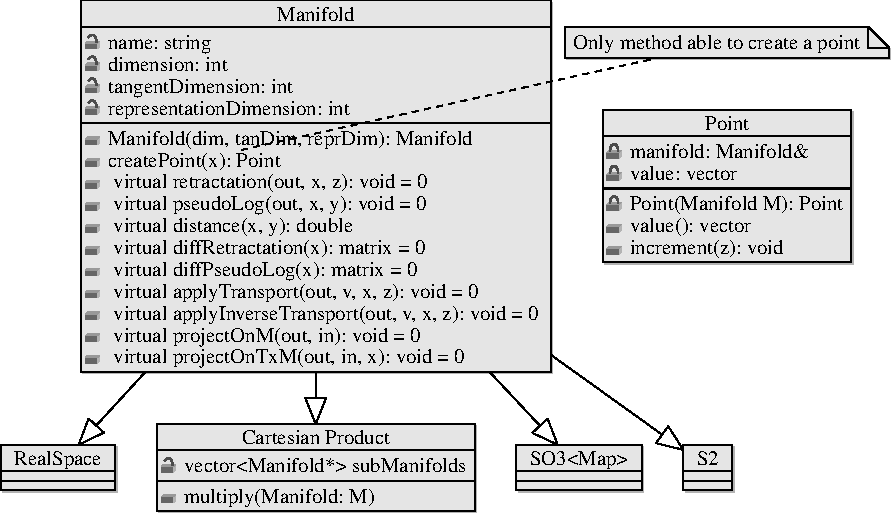
\includegraphics[width=\linewidth]{uml/manifolds-1.pdf}
  \caption{Simplified class diagram of the Manifold project}
\label{fig:uml_manifold}
\end{figure}

%}}}
%{{{ PRACTICAL IMPLEMENTATION
\section{Practical implementation}
\label{sec:practical_implementation}

The SQP algorithm presented in Section~\ref{local_sqp_on_manifolds} works locally, \emph{i.e.} when starting close enough to the solution.
In practice, various refinements are made to ensure convergence from any starting point.
We detail hereafter our choices.

\subsection{Linear and quadratic problems resolution}
\label{sub:linear_and_quadratic_problems_resolution}

The central idea of an SQP algorithm is that it solves a series of QP problems iteratively.
There are many off-the-shelf QP solvers available and the state of the art is mature in that field, thus, we decided to use the LSSOL solver~\cite{gill:techrep:1986}.
LSSOL provides resolution methods for several types of problems and we are interested in using the FP (Feasibility Problem) and QP.\@
The LSSOL framework formulates problems as follows (Note that there are no equality constraints in this formulation):

\begin{align}
  \minimize_{x\in \mathbb{R}^n}\ &{F(x)}\\
  \text{subject to}\  & l\leq \begin{Bmatrix}
    x\\
    Cx
  \end{Bmatrix}
  \leq u
\end{align}

With the $F$ function taking different forms depending on the problem to solve:
\begin{table} [H]
\centering
\begin{tabular}{ccc}
  \toprule
  FP:\@ & None & (find a feasible point for the constraints)\\
  \midrule
  QP2: & $c^T+\frac{1}{2} x^T A x$ & A symmetric and positive semi-definite \\
  \midrule
  QP4: & $c^T+\frac{1}{2} x^T B^T B x$ & A $m\times n$ upper-trapezoidal \\
  \bottomrule
\end{tabular}
\end{table}

The QP4 type of problem is used when a decomposition of the matrix $A$ of QP2, $A=B^T B$ is available.

\subsection{Problem Definition}
\label{sub:problem_definition}

As stated in Eq~\ref{eq:pb_on_SO3} we want to solve a non-linear constrained optimizarion problem on manifold that takes the following form:

\begin{align}
  \minimize_{x \in \mathcal{M}} & \quad f(x)\\
  \text{subject to}&
  \begin{array}{lr}
    l \leq c(x) \leq u \nonumber
  \end{array}
\end{align}

The list of constraints can be separated in 3 categories: Bounds, Linear and Nonlinear.
For convenience, we formulate our optimization problem in a way that is compatible with LSSOL by changing all equality constraints into inequality constraints:

\begin{equation}
  c(x) = 0 \Leftrightarrow 0 \leq c(x) \leq 0
\end{equation}

Our problem can be written:
\begin{align}
\label{eq:optim_problem_on_manifold}
  \minimize_{x \in \mathcal{M}} & \quad f(x)\\ \nonumber
  \text{subject to}&\left\{
  \begin{array}{lr}
    L_B \leq x \leq U_B \\
    L_L \leq Ax \leq U_L \\
    L_N \leq c(x) \leq U_N
  \end{array}\right.
\end{align}

With $L_B$ and $U_B$ being respectively the lower and upper bounds for Bounds constraints, $L_L$ and $U_L$ the lower and upper bounds for Linear constraints, and $L_N$ and $U_N$ the lower and upper bounds for Nonlinear constraints.
That formulation is convenient and used to define our problem, but since we are solving this problem on a non-Euclidean manifold, we need to re-formulate the problem around the current iterate $x_i$ at each iteration.
This is done automatically behind the scene and the user only has to provide the informations to build problem~\ref{eq:optim_problem_on_manifold}.

At iteration $i$, the problem becomes (for clarity, we drop the subscript $i$ that goes with each appearance of $x$):
\begin{align}
\label{eq:optim_problem_on_txm}
  \minimize_{\mathbf{z} \in T_x\mathcal{M}} & \quad f(\varphi_x(\mathbf{z}))\\ \nonumber
  \text{subject to}&\left\{
  \begin{array}{lr}
    {\bf z}_{\text{map}}^- \leq \mathbf{z} \leq {\bf z}_{\text{map}}^+ \\
    L_B \leq \varphi_x(\mathbf{z}) \leq U_B \\
    L_L \leq A\varphi_x(\mathbf{z}) \leq U_L \\
    L_N \leq c(\varphi_x(\mathbf{z})) \leq U_N
  \end{array}\right.
\end{align}

With ${\bf z}_{\text{map}}^-$ and ${\bf z}_{\text{map}}^+$ being respectively the lower and upper bounds of validity of the tangent map of $\mathcal{M}$ around $x$.
After this reformulation, we note that if $\varphi_x$ is nonlinear, then the bounds and linear constraints of problem~\ref{eq:optim_problem_on_manifold} became nonlinear in problem~\ref{eq:optim_problem_on_txm}.
It is then necessary to treat the problem and evaluate which constraint is linear and which is not in order to go back to a formulation of the same type as in problem~\ref{eq:optim_problem_on_manifold}.
Basically, for each constraint $c_j$ in problem~\ref{eq:optim_problem_on_txm}, if the submanifold of $\mathcal{M}$ on which that constraint is applied is a realspace $\mathbb{R}^m$ then the constraint maintains its bound, linearity or nonlinearity status, otherwise, it becomes a nonlinear constraint\footnote{At the time I am writing those lines. This treatment of the constraints is a planned work, it has not been implemented yet.}.
Once again, this may look like a drawback of optimization on manifolds, but it is usually the same with classical optimization.
Indeed, a linear constraint on the representation space of a non-Euclidean manifold might not often make much sense.
For example, a linear constraint on the elements of a unit-quaternion, although one can obviously be devised, does not seem to make much sense.

In the particular case of linear constraints (and by extension bound constraints) on a submanifold that is a realspace, the constraints on $x$ are transformed into constraints on $z$ as follows:
\begin{equation}
  L_L \leq Ax \leq U_L \ \Rightarrow \ L_L - Ax \leq A\mathbf{z} \leq U_L-Ax
\end{equation}
For bounds constraints, the same goes with $A$ as the identity matrix on the submanifold.

Once those substitutions are done, we obtain a problem of the following form (note that $L_B$, $L_L$, $L_N$, $U_B$, $U_L$, $U_N$, $A$ and $c$ are not the same as in problem~\ref{eq:optim_problem_on_manifold}):

\begin{align}
\label{eq:optim_txm_final}
  \minimize_{\mathbf{z} \in T_x\mathcal{M}} & \quad f \circ \varphi_x(\mathbf{z})\\ \nonumber
  \text{subject to}&\left\{
  \begin{array}{lr}
    L_B \leq \mathbf{z} \leq U_B \\
    L_L \leq A \mathbf{z} \leq U_L \\
    L_N \leq c \circ \varphi_x(\mathbf{z}) \leq U_N
  \end{array}\right.
\end{align}

This problem is an exact reformulation of problem~\ref{eq:optim_problem_on_manifold} on $T_x\mathcal{M}$.
At each step of the optimization process, we solve the quadratic problem approximating this problem~\ref{eq:optim_txm_final} around $\mathbf{z}=0$.
The Taylor development of $c\circ\varphi_x(z)$ to the first order around $\mathbf{z} = 0$ gives:
\begin{equation}
  c \circ \varphi_x(\mathbf{z}) \approx c\circ \varphi_{x_k}(0) + \frac{\partial c\circ \varphi_{x_k}}{\partial {\bf z}}(0) {\bf z } = c(x_k) + {\left(\nabla\varphi_{x_k}(0) \nabla c (x_k)\right)}^T\mathbf{z}
\end{equation}

The QP to solve at each iteration is the following:

\begin{align}
  \label{eq:QP_txm}
  \begin{split}
  \minimize_{\mathbf{z} \in T_x\mathcal{M}=\mathbb{R}^n } & \quad {\left(\nabla\varphi_{x_k}(0) \nabla f (x_k)\right)}^T\mathbf{z} + \frac{1}{2} {\bf z }^T H_k{\bf z }\\
  \text{subject to}&\left\{
  \begin{array}{lr}
    L_B \leq \mathbf{z} \leq U_B \\
    L_L \leq A \mathbf{z} \leq U_L \\
    L_N \leq c(x_k) + {\left(\nabla\varphi_{x_k}(0) \nabla c (x_k)\right)}^T\mathbf{z}\leq U_N\\
  \end{array}\right.
  \end{split}
\end{align}

The resolution of this QP~\ref{eq:QP_txm} (with LSSOL) gives the optimal solution $\mathbf{z}^*$ and Lagrange multipliers $\lambda^*$.
The new iterate that will be considered is:
\begin{equation}
  x_{k+1}\leftarrow \varphi_{x_k}(\mathbf{z}^*)
\end{equation}

\subsection{Trust-region and limit map}
\label{sub:trust_region_and_limit_map}

Maps $\varphi_{x}$ are only valid locally, and we need to account for this: a step ${\bf z}$ found by Problem~(\ref{eq:QP_txm}) should not be outside the validity region of the map.
We could enforce this by adding the limits of the manifold map to the problem as bound constraints.
In fact, this comes down to intersecting the original problem's bounds with the limits of the map and imposing the resulting bounds as constraints.
This leads naturally to trust region methods that we therefore favor over line-search approaches.
We present the classical trust-region strategy in Section~\ref{ssec:the_trust_region_strategy}.
In the case of a robotics problem, different variables often have different orders of magnitude, for example, contact forces can be of the order of $100N$ while joint angles are of the order of $1rad$.
Let $x$ be the variable vector of such problem with $x=[\theta_0, \theta_1, f_0, f_1, f_2]^T$ where $\theta$ represents an angular variables and $f$ a force.
The shape of the trust-region should reflect those differences, but we want to keep the simplicity of the classical trust-region strategy.
For that, we propose to separate the trust-region $\rho$ in two parts: its scale $\rho_\text{scale}$ which is a scalar, and its shape $\rho_\text{shape}$ which in a vector of dimension $n$, the dimension of $\mathcal{M}$ (that value is actually stored in the instance of manifold).
$\rho_\text{shape}$ is set at the beginning of the optimization and is a constant, it represents the size of the trust-region in every directions.
In the previous example, we'd get ${\rho_\text{shape}} = [1,1,100,100,100]^T$
And $\rho_\text{scale}$ is the scalar that gets updated during the trust-region strategy.

Finally, the constraints related to the trust-region added to the problem come down to:
\begin{equation}
  -\rho = -\rho_\text{scale}\rho_\text{shape} \leq \mathbf{z} \leq \rho_\text{scale}\rho_\text{shape} = \rho
\end{equation}

\subsection{Filter method}
\label{sub:filter_method}

To know if a step ${\bf z}$ is acceptable or not, one usually uses a penalty-based merit function.
In our early tests, the update of the penalty parameters proved to be difficult with our types of problems.
We now use a filter instead.

Our algorithm is an adaptation of Fletcher's filter SQP~\cite{fletcher:mathprog:2000} to the case of manifolds: we use an adaptive trust-region that is intersected with the validity region of $\varphi_{x_i}$, and a new iterate $x_{i+1} = \varphi_{x_i}({\bf z})$ is accepted if either the cost function or the sum of constraint violations is made better than for any previous iterates.

\subsection{Hessian update on manifolds}
\label{sub:hessian_update_on_manifolds}

Aside from the manifold adaptation, our main departure from Fletcher is in the Hessian computation where we used an approximation, since the exact one is too expensive to compute in our problems.
After testing several possibilities, we settled for a self-scaling damped BFGS update~\cite{nocedal:mp:1993,nocedal:book:2006}, adapted to the manifold framework.
More precisely, given the Hessian approximation $H_k$ at iteration $k$, we compute the approximation $H_{k+1}$ as follows
\begin{align}
  &s_k = \mathcal{T}_z(z), \quad y_k = \nabla_z \mathcal{L}_{x_{k+1}}(0,\lambda_{k+1}) - \mathcal{T}_z(\mathcal{L}_{x_{k}}(0,\lambda_{k})) \nonumber\\
  &\theta_k = \left\{\begin{array}{ll}
    1 & \mbox{if} \; s_k^T y_k \geq 0.2 s_k^T \tilde{H}_k s_k \\
    \frac{0.8 s_k^T \tilde{H}_k s_k}{s_k^T \tilde{H}_k s_k - s_k^T y_k} & \mbox{otherwise}
  \end{array}\right. \nonumber\\
  &r_k = \theta_k y_k + \left(1-\theta_k\right) \tilde{H}_k s_k \quad \mbox{(damped update)} \nonumber\\
  &\tau_k = \min\left(1, \frac{s_k^T r_k}{s_k^T \tilde{H}_k s_k} \right) \quad \mbox{(self-scaling)} \nonumber\\
  &H_{k+1} = \tau_k \left(\tilde{H}_k-\frac{\tilde{H}_k s_k s_k^T \tilde{H}_k}{s_k^T \tilde{H}_k s_k} \right) + \frac{r_k r_k^T}{s_k^T r_k} \nonumber%
\end{align}
where $\mathcal{T}_{\bf z}$ is a vector transport along ${\bf z}$ (see~\cite{absil:book:2008}) and $\tilde{H}_k$ is such that for ${\bf u} \in T_{x_{k+1}} \mathcal{M}$, $\tilde{H}_k {\bf u} = \mathcal{T}_{\bf z}\left(H_k \mathcal{T}_{\bf z}^{-1}({\bf u}) \right)$.

\subsection{Hessian Regularization}
\label{sub:hessian_regularization}

Despite Powell's update, $H_{k}$ might not be positive definite (but still symmetric).
We regularize it as follows: we first perform a Bunch-Kaufman factorization $P_k H_k P_k^T= L_k B_k L_k^T$ where $P_k$ is a permutation matrix, $L_k$ is unit lower triangular and $B_k$ is block diagonal with blocks of size $1 \times 1$ or $2\times 2$ (obtaining $B_k$ as a diagonal matrix is not numerically stable for Cholesky-like decomposition of indefinite matrices), see~\cite{golub:book:1996}.
The eigenvalue decomposition $B_k = Q_k D_k Q_k^T$ is immediate and cheap to compute.
From the diagonal matrix $D_k$ we form $D'_k$ such that $d'_{ii} = \max\left(d_{ii},\mu_{\min}\right)$ where $\mu_{\min}>0$ is user-defined (we typically set it to $0.1$).
Defining $L'_k = L_k Q_k {(D'_k)}^{1/2}$, we get a regularized matrix $H'_k = P_k^T L_k L_k^T P_k$.
In our case, we use {\tt LSSOL}~\cite{gill:techrep:1986} for solving the QP~(\ref{eq:SQPStep}), which directly accepts the factorized form $(P_k, L'_k)$.
This avoids an internal Cholesky factorization so that our regularization does not add too much time to the overall process of building and solving the QP.\@

%}}}



%%%%%%%%%%%%%%%%%%%%%%%%%%%%%%%%%%%%%%%%%%%%%%%%%%%%%%%%%%%%%%%%%%%%%%%
%                           Fourth Chapter                            %
%                       New Posture Generation                        %
%%%%%%%%%%%%%%%%%%%%%%%%%%%%%%%%%%%%%%%%%%%%%%%%%%%%%%%%%%%%%%%%%%%%%%%

\chapter{New Posture Generation}

%\section{List of contributions}
%\begin{itemize}
  %\item{Posture Generation, variables and architecture}
    %\begin{itemize}
      %\item Geometric expressions:
        %\begin{itemize}
          %\item Represent everything based on frames
          %\item Automatic derivative computation
        %\end{itemize}
      %\item Automatic mapping
      %\item Problem generator: a posture generation problem factory
    %\end{itemize}
  %\item{Problem Formulation: formulation of usual problems in the geometric expressions framework}
    %\begin{itemize}
      %\item Contact with plane surface
      %\item Static equilibrium: Newton/CoM projection
      %\item Forces in friction cones
      %\item Articular limits
      %\item Torque limits
      %\item Torque minimization
      %\item Goal Posture
    %\end{itemize}
  %\item{Implementation of new types of constraints in our formulation}
    %\begin{itemize}
      %\item Contact with parametrized surfaces on Rn
      %\item Contact with parametrized surfaces on S2: Sphere, SuperEllipsoid
      %\item Contact with Catmull-Clark Subdivision surfaces
    %\end{itemize}
  %\item{Contact with desired force}
  %\item{Potential contacts}
  %\item{Simulation Results}
  %\item{Multi-Robot}
%\end{itemize}

Writing a posture generation problem can easily become cumbersome without the appropriate tools.
Common pitfalls are for example writing the derivative of a function, managing how the Jacobian matrices of the already implemented functions are modified when a variable is added to the problem, adding a new type of constraint, or correctly writing a function on a sub-manifold of the problem manifold.
A fair amount of bookkeeping is always necessary, which should not be the charge of the user writing the constraints.
In our PG, we propose an architecture automating most of the problematic tasks, so that the user can focus on the mathematical formulation of the problem:
\begin{itemize}
  \item A system of geometrical and mathematical expression trees that automatically computes the mathematical expressions behind geometric relations
  \item An automatic mapping between the submanifold of each function and the global manifold of the problem
  \item A problem generator that aggregates all the informations from the abovementionned items to generate an optimization problem that can be passed to the solver
\end{itemize}


\section{Geometric expressions}
\label{sec:geometric_expressions}

Most constraints are geometric.
In order to simplify the writing of functions, we use a dedicated system of expression graph encapsulated in a set of geometric objects.
The main idea is to separate the purely mathematical logic from the geometric one.
As an example if $P_r$ and $V_r$ are a point and a vector attached to the camera of the robot, and $P_e$ is a fixed point in the environment, the constraint $(P_e - P_r).V_r = 0$ can be used to have the robot look at $P_e$.
With our system, the user creates only those objects and write the code {\tt (Pe-Pr).dot(Vr)} to get the value needed.
The geometric layer takes care that all the quantities are expressed in the correct frame, the mathematical layer performs the corresponding operations.
If $q$ is a variable object, {\tt (Pe-Pr).dot(Vr).diff(q)} returns automatically the differential of the expression w.r.t. $q$. This makes the writing of the constraints very easy.

At the mathematical level, we consider 5 types of expressions which can be either variables or constants:
\begin{itemize}
  \item Scalar, a 1-dimensional element of $\mathbb{R}$
  \item Coordinates, a 3-dimensional element of $\mathbb{R}^3$
  \item Rotation, a $3\times3$ matrix representing a 3D rotation
  \item Transformation, a $4\times4$ matrix representation of a 3D isometry
  \item Array, a dynamic size array
\end{itemize}
The meaningful unary (inverse, opposite, norm\ldots) and binary (multiplication, addition, subtraction, dot product\ldots) operations (with their derivatives by chain rule) are implemented.
We also have a Function class for more complicated expressions, for example expressing $q \mapsto T_i(q)$ where $T_i$ is the transformation between the reference frame of the robot and the frame of its $i$-th body~\footnote{The kinematics of rigid body systems is handled by the RBDyn library (\url{https://github.com/jorisv/RBDyn})}.
The combinations of those elementary operations defines a computation graph, just like in many symbolic calculation frameworks.

The geometric layer consists of physical or geometric objects, named features, which exist independently of their mathematical expression in a given reference frame.
We have so far 4 objects:
\begin{itemize}
  \item A Frame, defined by a Transformation expression and a reference frame.
  \item A Point and a Vector, defined by a Coordinates expression and a reference frame.
  \item A Wrench, defined by a pair of Coordinates expressions and a reference frame.
\end{itemize}
We have a special World Frame object to serve as starting reference frame.

For each feature, one can get its expression in a given frame.
Basic operations are defined between those features (when applicable).
For example, the subtraction between two Points gives a Vector.
The geometric logic resides in the change of frame and those operations.

%Based on that expression system, the robot can simply be represented as a function that keeps track and updates the transformations of the frames of all its bodies, with respect to an Array expression on entry, the articular parameters.
%For a given articular parameter array, the user can query the frame of any body on the robot, and by composition, the user can query any feature defined on a frame of the robot, as well as its derivatives.
%This tools allows for a simplified writting of robotics constraints as a combination of operations on geometric features, without worrying about the vectors and matrix beneath and without having to write the derivatives.

\section{Automatic mapping}
\label{sec:automatic_mapping}

The manifold $\mathcal{M}$, on which the optimization takes place, is a Cartesian product of several sub-manifolds. Same goes for their representation spaces:
\begin{equation}
  \begin{split}
    \mathcal{M} = \mathcal{M}_1\times\mathcal{M}_2\times\mathcal{M}_3\times\hdots\\
    \mathbb{E} = \mathbb{E}_1\times\mathbb{E}_2\times\mathbb{E}_3\times\hdots
  \end{split}
\end{equation}
From the solver's viewpoint, the entry space of each function is the complete manifold.
But for the developer, writing a function on the complete $\mathbb{E}$ is cumbersome because (i) of the need to manage indexes, and (ii) when the function is implemented, the complete $\mathbb{E}$ may not be known.
A user-written function $f$ is usually defined on a subset of $\mathbb{E}$, say $\mathbb{E}_I=\mathbb{E}_i\times\mathbb{E}_j\times\mathbb{E}_k\hdots$, that is minimalist for that function, and should not account for unrelated manifolds.
One does not want to think about the values of the forces when writing a geometric constraint for example.
Our automatic mapping tool keeps track of all the necessary mappings for each function added and upon the instantiation of the problem, generates the correct projection functions $\pi_I$ such that the developer can write a function $f$ on $\mathbb{E}_I$ while the solver receives it as a function $f \circ \pi_I$ on $\mathbb{E}$.
This idea is illustrated by the example in Fig.~\ref{fig:auto_map}
%\begin{equation}
  %\begin{split}
  %\pi_I:\mathbb{E}\to\mathbb{E}_I\\
  %f:\mathbb{E}_I\to\mathbb{R}\\
  %f\circ\pi_I:\mathbb{E}\to\mathbb{R}
  %\end{split}
%\end{equation}

\begin{figure}[!htb]
\centering
  \centering
  \setlength\fboxsep{0pt}
  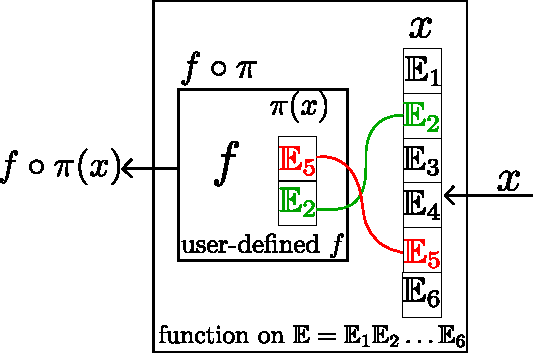
\includegraphics[width=.5\linewidth]{Chapter4-NewPG/Figs/auto_mapping_text.pdf}
\caption{automatic variable mapping}
\label{fig:auto_map}
\end{figure}

\section{Problem Generator}
\label{problem_generator}

The problem generator is the tool constructing the optimization problem.
It registers all the variables and the functions related to a given problem.
Each function is likely to bring additional variables with it.
For each contact contributing to the balance, a variable on $\mathbb{R}^3$ representing the contact force is added to the problem.
The associated wrench is added to the stability constraints.
Once the registration is complete, the complete manifold of the problem is generated and uses the information of the Automatic mapping to `plug' each function with the correct sub-manifold.
Subsequently, the optimization problem can be generated and passed to the solver.
The communication between the solver and the generated problem is made through the RobOptim framework\footnote{\url{http://www.roboptim.net/}}~\cite{moulard:jsme:2013, moulard:jrsj:2014}.

\section{Problem formulations}
\label{sec:problem_formulations}

Let $q=[q_F^T; q_r^T]\in\mathbb{R}^3\times SO(3)\times \mathcal{M}_r$ be the combination of the free-flyer of the robot $q_F\in \mathbb{R}^3 \times SO(3)$ and the articular parameters $q_r\in\mathcal{M}_r$.
Let $\mathcal{W}_i(p)=\{f_i,m_i(p)\}$ be the wrench (force+moment) applied by the environment onto the robot at contact $i$ and expressed on point $p$.
A frame $F$ is composed of a reference point and an orthonormal basis of 3 vectors $F = \{O, (x, y, z)\}$.

Here is a list of constraints that we consider in our problem (implementation of other ones is on-going):
\begin{itemize}
\item Joint limits ${q^-} \leq q_r \leq {q^+}$:\\
These cannot be directly translated on manifolds other than $\mathbb{R}^n$.
For example, spherical joints can be parametrized on $S2 \times \mathbb{R}$, then the $S2$ part can be limited by a cone, and the $\mathbb{R}$ part can have real bounds.
\item The contact constraint consists in identifying the features of two frames $F_1$ and $F_2$.
For example, for a planar contact, we get the set of equation~\ref{eq:planar_contact}.

\begin{equation}
  \begin{split}
    \overrightarrow{O_1O_2}\cdot\vec{z_1} = 0\\
    \vec{z_2}\cdot\vec{z_1} \leq 0 \\
    \vec{z_2}\cdot\vec{x_1} = 0 \\
    \vec{z_2}\cdot\vec{y_1} = 0
  \end{split}
  \label{eq:planar_contact}
\end{equation}

Note that on $F_2$ only the point $O_2$ and the vector $z_2$ are necessary.
Other types of contacts can be created that way, by equalizing other features, as explained in~\cite{escande:ras:2013}.

\item The stability constraint ensures that the Euler-Newton equation~(\ref{eq:NewtonWrench}) is balanced for the set of external wrenches applied to the robot (gravity $\mathcal{W}_G$ and contact forces $\mathcal{W}_i$).
  \begin{equation}
    \sum_{i}{\mathcal{W}_i(p)} + {\mathcal{W}_G(p)} = 0
    \label{eq:NewtonWrench}
  \end{equation}
  For each contact that bears forces (`stability' contact), a wrench applied on the robot at the contact point is added to the problem.
  That wrench is parametrized on a subset of $\mathbb{R}^6$ depending on the type of contact.
  For punctual contacts, the moment part is null on the application point.
  Only a parametrization of the force part on $\mathbb{R}^3$ is needed.
  We model planar contacts as a combination of punctual forces applied at each vertex of the contact polygon.
  In the case of interaction forces between 2 robots, only one wrench is created and it is used as is in the stability equation of one robot and its opposite is used for the stability of the second robot.

\item The friction cone constraint limits the tangential part of every forces to avoid slippage.
We write it as~\ref{eq:friction} (with $\mu$ the friction coefficient)
\begin{equation}
  \begin{split}
    \mu^2f_z^2-f_x^2-f_y^2 \geq 0 \\
    f_z \geq 0
  \end{split}
  \label{eq:friction}
\end{equation}
\end{itemize}

The frame in which the constraints are written matters critically.
Most often, the frame's configuration depends on a part of the optimization variables, that must be accounted for in computing the constraints' Jacobian.
Our framework computes such dependencies automatically.

Our current PG (i.e.\ coding state) does not include yet collisions and auto-collisions, nor torque limits.
Their implementation is on-going and is simply the matter of coding time.
Another important part is its cost function.
We only mention the cost function that have specificities when dealing with manifolds, the distance to a reference posture $q_0$.
On a robot that has all its articulations parametrized on $\mathbb{R}$ the distance can be expressed simply with the Euclidean norm $d = \norm{q_j-q_0}^2$.
Since we work on non-Euclidean manifolds, the logarithm function on the manifold must be used.
It gives the distance vector between two points in the tangent space, the norm of this vector can be used as a distance.
So we get $d = \norm{\text{log}_{q_0}(q_r)}^2$.


%FROM HERE IT IS OLD TEXT

%There can be several kinds of contact between a surface of the robot and its environment(which could contain other robots).
%We denote $\mathcal{S}_R$ and $\mathcal{S}_E$ the two surfaces belonging to two bodies $\mathcal{B}_R$, $\mathcal{B}_E$ that are to be put in contact.
%We equip those surfaces with a frame $\mathcal{F} = \{O, (x, y, z)\}$, with $O$ a point of contact on the surface, and $z$ a vector normal to the surface at $O$.
%The transformation that leads from the reference frame of a body $\mathcal{B}$ to the reference frame of a surface $\mathcal{S}$ is denoted $^\mathcal{S}H_\mathcal{B}$.
%Note that those two surfaces do not need to be plane, a curved continous surface would suit as well.
%For a contact to be geometricaly satisfied, the planes defined by $\{O, (x, y)\}$ on both surfaces must be coplanar with normals of opposite directions.
%This can be assured by satisfying the following set of equation:

%\begin{align}
  %\begin{split}
  %(O_R-O_E) . z_E = 0 \\
  %z_R . x_E = 0 \\
  %z_R . y_E = 0 \\
  %z_R . z_E \leq 0
  %\end{split}
  %\label{eq:floating contact}
%\end{align}

%If any(either or both) of the two surfaces in contact is non-plane, finding the exact location of the contact point on the surface is necessary, because then, the normal to the contact is not known in advance.
%In that situation, we propose to paramaterize the contact frame on the surface on a 1 or 2-dimentional manifold.
%\begin{equation}
  %\mathcal{F}(u_S\in \mathcal{M}_S) = \{O(u_S), (x(u_S), y(u_S), z(u_S)\}
%\end{equation}
%Which, depending on the shape, could be $\mathbb{R}^2$ or $S2$.
%In that case, an additional set of variables $u_S\in \mathcal{M}_S$ is added to the optimization problem as well as the constraint set \ref{eq:floating contact} depending on it.

%The floating contact constraint can be extended to fix the contact to a given position and orientation by adding to it the following set of equation that locks the degrees of freedom of rotation around the normal and translation in the tangent plane of the contact:

%\begin{align}
  %\begin{split}
  %(O_R-O_E) . x_E = 0 \\
  %(O_R-O_E) . y_E = 0 \\
  %y_R . x_E = 0 \\
  %x_R . y_E = 0
  %\end{split}
  %\label{eq:fix planar contact}
%\end{align}

%Those two sets of equations \ref{eq:floating contact} and \ref{eq:fix planar contact} can easily be recombined to generate other types of constraints(e.g. fixing only the translation, or only the rotations...).

%For any scenario to be realistic, the robot must satisfy its stability constraint. Given a set of wrenches applied on the robot $\{\mathcal{W}_0, \mathcal{W}_1...,\mathcal{W}_{n_w}\}$.
%The sum of all those wrenches applied on a singular point must be zero.
%For each punctual contact that needs to bear forces, a new wrench is created, that wrench is parametrized by a set of two vectors describing its force $f = (f_x, f_y, f_z)^T \in \mathbb{R}^3$ and moment $m = (m_x, m_y, m_z)^T \in \mathbb{R}^3$ at the contact point.
%We denode $\mathcal{W}_G$ the wrench generated by the weight of the robot: $\mathcal{W}_G(CoM) = \{(0, 0, -mg)^T, (0, 0, 0)^T\}$.
%For any chosen reduction point $p$, the stability constraint writes as follows:

%\begin{equation}
  %\sum_{i=0}^{n_w}{\mathcal{W}_i(p)} + {\mathcal{W}_G(p)} = 0
  %\label{eq:NewtonWrench}
%\end{equation}

%Equation \ref{eq:NewtonWrench} can be rewritten with only vectors as:

%\begin{equation}
  %\begin{split}
  %\sum_{i=0}^{n_w}{f_i} - m g = 0 \\
  %\sum_{i=0}^{n_w}{m_i(p)} + {m_G(p)} = 0
  %\end{split}
  %\label{eq:NewtonForceMoment}
%\end{equation}

%A usual choice of reduction point for those equations is the center of mass of the robot.
%In which case the moment part of the gravity wrench is null.
%In the case of surfacic contact between two plane surfaces, the contact polygon is determined and a punctual force with zero moment is added on each vertex.
%The forces generated on each point need to satisfy the Coulomb friction cone equations which writes as follows for a friction coefficient $c$:

%\begin{equation}
  %\begin{split}
    %c^2 f_z^2 - f_x^2 - f_y^2 \geq 0 \\
    %f_z \geq 0
  %\end{split}
  %\label{eq:FrictionCone}
%\end{equation}

%It is not straightforward to devise a friction limit in terms of moment.
%Which is why, in the current study, we considere that the punctual contacts are perfect and do not generate moment on their application point.
%This translates in fixing the moment variables of the wrench to zero while the force variables still exist.
%In the case of planar contacts, of course, the moment part cannot be ignored.
%But, given a planar polygon in which the contact happens, the wrench generated by this contact can be modeled as a set of punctual forces, one on each vertex of the polygon.
%Which respect the same friction cone equations \ref{eq:FrictionCone} and are taken into account in \ref{eq:NewtonWrench}.

%\section{Posture Generation, variables and architecture}
%\label{sec:posture_generation_variables_and_architecture}

%\section{Problem Formulation}
%\label{sec:problem_formulation}

%\section{Simulation Results}
%\label{sec:simulation_results}

%\section{Parametrization of complex solids on S2}
%\label{sec:parametrization_of_complex_solids_on_s2}

%\section{Potential contacts}
%\label{sec:potential_contacts}

%\section{Optimization of the solvers parameter for a class of problems}
%\label{sec:optimization_of_the_solvers_parameter_for_a_class_of_problems}


%%%%%%%%%%%%%%%%%%%%%%%%%%%%%%%%%%%%%%%%%%%%%%%%%%%%%%%%%%%%%%%%%%%%%%%
%                            Fifth Chapter                            %
%                   Evaluation and Experimentations                   %
%%%%%%%%%%%%%%%%%%%%%%%%%%%%%%%%%%%%%%%%%%%%%%%%%%%%%%%%%%%%%%%%%%%%%%%

\chapter{Evaluation and Experimentation}
\label{cha:evaluation_and_experimentation}

\section{List of contributions}
\begin{itemize}
  \item Understanding the environment through a point-cloud
    Extraction of plane polygons from Kinect acquired point-clouds.
    Segmentation pipeline:
    \begin{itemize}
      \item Acquisition
      \item Filtering
      \item Region growing segmentation
      \item Planar Extraction
      \item Planar projection and Hull convex generation
      \item Re-orientation and transfer to the planner
    \end{itemize}
  \item Generation of sequences of postures on segmented environment
  \item{Simulated scenarios planned on real-environment: HRP-2 climbing on table through stairs, HRP-2 climbing on table through slope}
  \item{Machine Learning: Optimization of the solvers parameter for a class of problems}
    \begin{itemize}
      \item Developpement of a list of typical robotics optimization problem
      \item Training of a genetic algorithm to find the "best" solver tuning to solve a family of problems
    \end{itemize}
  \item{Several scenarios, including Airbus}
\end{itemize}



%%%%%%%%%%%%%%%%%%%%%%%%%%%%%%%%%%%%%%%%%%%%%%%%%%%%%%%%%%%%%%%%%%%%%%%
%                             Conclusion                              %
%%%%%%%%%%%%%%%%%%%%%%%%%%%%%%%%%%%%%%%%%%%%%%%%%%%%%%%%%%%%%%%%%%%%%%%

\chapter*{Conclusion}
\addcontentsline{toc}{chapter}{Conclusion}
\label{cha:conclusion}




% ********************************** Back Matter *******************************
% Backmatter should be commented out, if you are using appendices after References
%\backmatter

% ********************************** Bibliography ******************************
\begin{spacing}{0.9}

% To use the conventional natbib style referencing
% Bibliography style previews: http://nodonn.tipido.net/bibstyle.php
% Reference styles: http://sites.stat.psu.edu/~surajit/present/bib.htm

\bibliographystyle{apalike}
%\bibliographystyle{unsrt} % Use for unsorted references  
%\bibliographystyle{plainnat} % use this to have URLs listed in References
\cleardoublepage
\bibliography{References/SBbib} % Path to your References.bib file


% If you would like to use BibLaTeX for your references, pass `custombib' as
% an option in the document class. The location of 'reference.bib' should be
% specified in the preamble.tex file in the custombib section.
% Comment out the lines related to natbib above and uncomment the following line.

%\printbibliography[heading=bibintoc, title={References}]


\end{spacing}

% ********************************** Appendices ********************************

\begin{appendices} % Using appendices environment for more functunality


%%%%%%%%%%%%%%%%%%%%%%%%%%%%%%%%%%%%%%%%%%%%%%%%%%%%%%%%%%%%%%%%%%%%%%%
%                          Thesis Appendix A                          %
%                       Numerical Optimization                        %
%%%%%%%%%%%%%%%%%%%%%%%%%%%%%%%%%%%%%%%%%%%%%%%%%%%%%%%%%%%%%%%%%%%%%%%

\chapter{Numerical Optimization: Introduction}
\label{chapter:optimization}

\nomenclature[x-R]{$\mathbb{R}$}{Real space}
\nomenclature[x-R+]{$\mathbb{R}_\geq0$}{The set of positive Reals}
\nomenclature[x-S]{$\mathit{S}$}{Variable space}
\nomenclature[x-M]{$\mathcal{M}$}{A Manifold}
\nomenclature[x-T]{$T_x\mathcal{M}$}{The tangent space of manifold $\mathcal{M}$ at point x}
\nomenclature[a-F]{$F$}{The set of linearized feasible directions}
\nomenclature[a-f]{$f$}{Objective function}
\nomenclature[a-c]{$c_i$}{Constraint function}
\nomenclature[a-x]{$x$}{Optimization variable}
\nomenclature[a-xstar]{$x^*$}{Solution of the optimization problem}
\nomenclature[a-E]{${E}$}{Set of index for which constraints are equality constraints}
\nomenclature[a-I]{${I}$}{Set of index for which constraints are inequality constraints}
\nomenclature[x-L]{$\mathcal{L}(x,\lambda)$}{Lagrangian function of the optimization problem}
\nomenclature[G-o]{$\Omega$}{Feasible set}
\nomenclature[z-st]{s.t.}{subject to}
\nomenclature[z-KKT]{KKT}{Karush-Kuhn-Tucker first order optimality conditions}
\nomenclature[z-LICQ]{LICQ}{Linear Independence Constraints' Qualification}
\nomenclature[z-QP]{QP}{Quadratic Programming}
\nomenclature[z-IQP]{IQP}{Inequality constrained Quadratic Programming}

\graphicspath{{Appendix1-Optim/Figs/}}

%{{{SECTION: LIST OF CONTRIBUTIONS
%\section{List of contributions}
%\begin{itemize}
  %\item \sout{Introduction to optimization}
  %\item \sout{Notions of unconstrained optimization}
  %\item \sout{Notions of Constrained Optimization}
  %\item \sout{KKT}
  %\item Line Search
  %\item Trust Region
  %\item Filter
  %\item Merit function
  %\item SQP
  %\item Restoration phase
  %\item \sout{Hessian Approximation: BFGS, SR1}
%\end{itemize}
%}}}
\section{Introduction}
In modern science, optimization has an important place.
Mechanical engineers optimize the shape of structural parts.
Investors optimize the profit of a portfolio while minimizing the risks of loss.
Chemists optimize the efficiency and speed of reactions.
When it comes to robotics, optimization is widely used.
From the design of a robot to its actuation.
Any positioning of a robot requires the computation of the articular parameters of each joint of the robot, finding such parameters might be possible by using analytical methods for simple robots, but for robots as complex as humanoid robots, it is not possible.
Most often, an optimization process is used.

The goal of an optimization algorithm is to find an optimal solution $x^*$ to a problem.
Optimal in the sense that the solution is an optimum of a given objective function $f$.
And solution of a problem in the sense that it satisfies a set of $m$ constraints $\{c_i,\ i\in [1,m]\}$.
Both the constraints and the objective function are defined on the variable space $\mathit{S}$, which is the space in which the variable $x$ lives and in which we search a solution $x^*$ to our problem.

In order to present the principles of optimization, in this chapter, we will always consider that the variable space is $\mathit{S}=\mathbb{R}^n$.
We first consider unconstrained problems.
That type of problem will not be used in the rest of our dissertation, therefore, we will just present them shortly.
We will then focus on constrained optimization problems and the numerous methods used in their resolution.
We will particularly detail one specific constrained problem resolution algorithm that is the Sequential Quadratic Program (SQP).
The extension of those methods to solving problems on more complex variable spaces that are the non-Euclidean manifolds is the topic of Chapter~\ref{chapter:optimization_on_noneuclidean_manifolds}.

This Appendix does not pretend to give a fully detailed overview of numerical optimization methods, it gives the reader a quick overview of some key principles.
For more detailed information, we invite the reader to refer to the excellent books that we took inspiration from to write this chapter~\cite{nocedal:book:2006, bonnans:book:2003, boyd2004convex}.

\section{Unconstrained Optimization}

An unconstrained optimization problem consists of an objective function to minimize, without any constraint.
This problem, denoted $\mathcal{P}$, can be formulated as follows:

\begin{equation}
  \minimize_{x\in\mathbb{R}^n}\ {f(x)}
\label{eq:unconstrainedOptim}
\end{equation}

The classical approach to solve $\mathcal{P}$ is to use an iterative algorithm, starting from an initial guess $x_0$, and converging toward the solution $x^*$.
A very basic optimization scheme is presented in Algorithm~\ref{alg:basic_optim}.

\begin{algorithm}
\begin{algorithmic}
  \State{Starting from an initial guess $x_0$}
  \While{Convergence condition not met}
  \State{Compute descent direction $p_k$}
  \State{Update $x_{k+1}\leftarrow x_k + p_k$}
  \EndWhile{}
  \caption{Basic optimization scheme}
\label{alg:basic_optim}
\end{algorithmic}
\end{algorithm}

The objective function is not necessarily completely known, in the sense that we cannot always have an explicit formula. Often, the function $f$ is computed by another program that is able to compute $f(x)$, $\nabla_x f(x)$ and sometimes $\nabla_{xx} f(x)$ for a given value of $x$.
In order to have an efficient algorithm, we need to avoid any unnecessary computation of $f(x)$ and its derivatives.
We denote the values taken by $x$ along the iterations as $x_0$, $x_1$, $x_2$,\ldots $x_i$.
And $f(x_i)$ is denoted $f_i$.

Since our knowledge of the objective function is only partial, without further assumptions, it is not possible to guarantee that a point $x^*$ is a global solution:

\begin{equation}
  \text{$x^*$ is a global solution of $\mathcal{P}$ on $\mathit{S}$ } \equiv \forall x \in \mathit{S}, f(x^*) \leq f(x)
\end{equation}

Though, we can find a local solution $x^*$ of $\mathcal{P}$ (a local minimizer of $f$): such that there exist a neighborhood $\mathit{N}$ of $x^*$ where $\forall x\in \mathit{N}$, $f(x^*) \leq f(x)$.
Or even a strict local minimizer of $f$: such that there exist a neighborhood $\mathit{N}$ of $x^*$ where $\forall x\in \mathit{N}$, $f(x^*) < f(x)$.
That is the kind of solution that we are looking for and that our algorithms should find.

Under the assumption that the objective function is smooth and sufficiently continuous ($\mathcal{C}^2$), we have the following sufficient conditions for the optimality of $x^*$:

\begin{theorem}
  If $\nabla^2f$ is continuous in an open neighborhood of $x^*$, $\nabla f(x^*)=0$ and $\nabla^2 f(x^*)$ is positive definite.
  Then $x^*$ is a strict local minimizer of $f$.
\label{optimalityTheorem}
\end{theorem}

The same definition can be given for a local minimizer with $\nabla^2f(x^*)$ positive semi-definite.

There are several ways to choose a descent direction $p_k$ from an iterate $x_k$. The
most obvious one is probably the steepest descent direction $-\nabla f_k$. This
method provides the direction along which f decreases most rapidly and only
requires the evaluation of the first derivative of $f$, but that method can
become extremely slow on complicated problems. Another popular approach is the
Newton method, in which the objective function is approximated to the second
order

\begin{equation}
  f(x_k+p) = f_k + p^T\nabla f_k + p^T\nabla^2f_k p
\end{equation}

Then the chosen descent direction is the optimum of that approximated function,
the Newton direction.
\begin{equation}
  p^N_k = -{(\nabla^2 f_k)}^{-1} \nabla f_k
\end{equation}
The choice of this descent direction implies that the $\nabla^2f_k$ is positive
definite, in which case an adaptation of the definition of $p_k$ is required. Or
an approximation $B_k$ of $\nabla^2f_k$ that guarantees definite positiveness can be
used. %For example, the symmetric-rank-one (SR1) formula and the BFGS (Broyden,
%Fletcher, Goldfarb, Shanno) formula. Then the step becomes

\begin{equation}
  p_k = -B_k^{-1}\nabla f_k
\end{equation}

$p_k$ is then added to $x_k$ to compute $x_{k+1} \leftarrow x_k + p_k$ and the process is repeated until convergence is reached.

Many methods and refinements exist to solve this problem and some are presented in~\cite{nocedal:book:2006}.
Our main focus here is on methods to solve constrained problem as they arise in robotics.

%\subsection{Globalization methods (Section NEEDS TO BE REWRITTEN)}

%During the resolution of an optimization problem, the algorithm will generate a
%sequence of iterates $x_k$ starting from the initial iterate $x_0$ (Which is
%usually provided by the user). During the step $k$ of the optimization process,
%the solver, the current point is $x_k$ and we try to find $x_{k+1}$ such that
%$f(x_{k+1}) < f(x_k)$. There are several strategies to do that but we will only focus
%on 2 of them that are the most popular, the line-search and trust-region
%methods.

%\subsubsection{The Line-Search Strategy}
%In the Line-Search strategy, given a point $x_k$, a descent direction $p_k$ from this
%point is chosen and then a length of step is calculated to minimize the
%following 1-dimensional problem:
%\begin{align}
  %\minimize_{\alpha \in \mathbb{R}^+} f(x_k + \alpha.p_k)
%\label{eq:lineSearchNLP}
%\end{align}

%Once the best value of $\alpha$ has been found, the next iterate is computed:
%$x_{k+1} = x_{k} + \alpha p_k$ and the same process is repeated until a
%satisfying solution is found.

%It is not always necessary to find the optimal value of $\alpha$, especially if
%that is expensive. Indeed, $\alpha$ is only used to calculate the next iterate,
%from which another $p_k$ and $\alpha$ will be calculated. And in the end, the
%imprecision on the computation of $\alpha$ will be erased in the other steps of
%the resolution.

%There are several ways to choose a descent direction from an iterate $x_k$. The
%most obvious one is probably the steepest descent direction $-\nabla f_k$. This
%method provides the direction along which f decreases most rapidly and only
%requires the evaluation of the first derivative of $f$, but that method can
%become extremely slow on complicated problems. Another popular approach is the
%Newton method, in which the objective function is approximated to the second
%order

%\begin{equation}
  %f(x_k+p) = f_k + p^T\nabla f_k + p^T\nabla^2f_k p
%\end{equation}

%Then the chosen descent direction is the optimum of that approximated function,
%the Newton direction.
%\begin{equation}
  %p^N_k = -{(\nabla^2 f_k)}^{-1} \nabla f_k
%\end{equation}
%The choice of this descent direction implies that the $\nabla^2f_k$ is positive
%definite, in which case an adaptation of the definition of $p_k$ is required. Or
%an approximation $B_k$ of $\nabla^2f_k$ that guaranties definite positiveness can be
%used. For example, the symmetric-rank-one (SR1) formula and the BFGS (Broyden,
%Fletcher, Goldfarb, Shanno) formula. Then the step becomes

%\begin{equation}
  %p_k = -B_k^{-1}\nabla f_k
%\end{equation}

%\subsubsection{The Trust-Region Strategy}
%\label{ssec:the_trust_region_strategy}
%The Trust-Region Strategy works in an opposite way than the line-search one in
%the sense that during a line-search step, a direction is chosen, and based on
%that direction, a step-length is chosen. Whereas with a Trust-Region approach, a
%maximum step-length is chosen, and based on it, the descent direction and length
%are chosen.
%The principle of the trust region is that along the optimization process, a
%model of the problem is constructed and enriched at every step and at each step,
%the next iterate is the optimum of the model, with the constraint that the step
%to get there lies inside the trust-region. For example, let us consider that
%the trust region is a sphere of center $x_k$ and radius $\rho_k$, then the
%constraint on $p_k$ is $\|p_k\| \leq \rho_k$. A usual model to take for the
%objective function is the quadratic model with approximated Hessian
%\begin{equation}
  %m_k(p) = f(x_k+p) = f_k + p^T \nabla f_k + p^T B_k p
%\end{equation}
%And the optimization problem to solve at each step of the optimization is

%\begin{align}
  %\minimize_{p} & \quad f_k + p^T \nabla f_k + p^T B_k p \nonumber\\
%\text{s.t.}&
%\quad \|p\| \leq \rho_k
%\label{eq:trustRegionNLP}
%\end{align}

%Once the solution $p_k$ to this quadratic problem is found, its quality is
%estimated by evaluating the value of $f(x_k+p_k)$. If the actual decrease of $f$
%is satisfying (compared to the decrease predicted by the model) then the step is
%accepted and the size of the trust-region can be increased. Otherwise, the step
%is refused, the trust-region radius is reduced and a new step from $x_k$ is
%computed on that smaller trust region.

\section{Constrained Optimization}

Solving a constrained optimization problem consists in minimizing a cost function while satisfying a set of constraints.

A general formulation for such problems (that we denote $\mathcal{P}$) is:

\begin{equation}
  \label{formulation_NLCP}
  \mathcal{P} \equiv
  \left\{
  \begin{array}{l}
    \minimize\limits_{x\in\mathbb{R}^n}{f(x)}\\
    \text{ s.t. }
    \left\{
    \begin{array}{l}
      c_i(x) = 0,\ \forall i\in{E}\\
      c_i(x) \geq 0,\ \forall i\in{I}\\
    \end{array}
    \right.
  \end{array}
  \right.
\end{equation}

Where $f$ and $c_i$ are real-valued functions on a subset of $\mathbb{R}^n$.
$f$ is the objective function, and the $c_i$ are the constraint functions.
${I}$ and ${E}$ are sets of index such that $c_i,\ i\in{E}$ are the equality constraints, and $c_i,\ i\in{I}$ are the inequality constraints.

We define the feasible set $\Omega$ that contains all the feasible points (points satisfying the constraints) of $\mathcal{P}$.

\begin{equation}
  \Omega = \left\{ x\in \mathbb{R}^n:\ \forall i\in {E},\ c_i=0,\ \forall i\in{I},\ c_i \geq0\right\}
\end{equation}

The formulation~\ref{formulation_NLCP} can then be rewritten as:
\begin{equation}
  \label{formulation_NLCP_compact}
  \mathcal{P} \equiv \minimize_{x\in\Omega}{f(x)}
\end{equation}

In the general case, the problem~\ref{formulation_NLCP_compact} has multiple local solutions.
And finding the global minimizer of $f$ in $\Omega$ is a difficult problem that we do not treat in this thesis.
Our goal is to find a local minimizer $x^*$ of $f$ in $\Omega$.

\subsection{Optimality conditions}
\label{sub:optimality_conditions}

\paragraph{First-Order Optimality Conditions}

The First Order Optimality Condition (Karush-Kuhn-Tucker Condition) is a necessary condition verified by all solutions of problem~\ref{formulation_NLCP}.

We introduce the Lagrangian function of~\ref{formulation_NLCP}:
\begin{equation}
  \mathcal{L}(x,\lambda) = f(x) + \sum_{i\in E\cup I}\lambda_i c_i(x)
\end{equation}

Any given constraint $c_i$ is said to be active at $x$ if $c_i(x)=0$.
In particular, for any feasible point $x$, all equality constraints $c_i,\ i\in E$ are active.
An inequality constraint $c_i,\ i\in I$ is inactive if $c_i(x)>0$ and active if $c_i(x) = 0$

\begin{definition}
\label{active_set}
  The active set $\mathit{A}(x)$ at a feasible point $x$ is the set of all the indexes of active constraint.
  \begin{equation}
    \mathit{A}(x)=E\cup\{i\in I: c_i(x) = 0\}
  \end{equation}
\end{definition}

Most optimization algorithms make the assumption that at the solution, the constraints satisfy the following Linear Independence Constraints' Qualification (LICQ) definition:

\begin{definition}
  Given a point $x$ and an active set $\mathit{A}(x)$, we say that the LICQ holds if the set of active constraint gradient $\{\nabla c_i(x),\ i\in \mathit{A}(x)\}$ is linearly independent
\end{definition}

In general, if LICQ holds, none of the active constraints gradients can be zero.
%In particular, if any gradient of a constraint is null, then the LICQ does not hold.
%The LICQ should be taken into account during the formulation of a problem.

\begin{theorem}{First-Order Necessary Conditions}\\
\label{KKT_conditions}
  Suppose that $x^*$ is a local solution of~\ref{formulation_NLCP}, that the functions $f$ and $c_i$ are continuously differentiable, and that the LICQ holds at $x^*$.
  Then there is a Lagrange multiplier vector $\lambda^*$, with components $\lambda_i^*$, $i\in E\cup I$, such that the following conditions are satisfied at $(x^*,\lambda^*)$
  \begin{equation}
  \begin{array}{ll}
    \nabla_x\mathcal{L}(x^*,\lambda^*) = 0 &, \\
    c_i(x^*) = 0 &,\ \forall i\in E\\
    c_i(x^*) \geq 0 &,\ \forall i\in I\\
    \lambda_i^* \geq 0 &,\ \forall i\in I\\
    \lambda_i^* c_i(x^*)=0 &,\ \forall i \in E\cup I\\
  \end{array}
  \end{equation}
\end{theorem}

In many cases, the main goal of an optimization algorithm is to find a point that satisfies the KKT conditions.

\paragraph{Second-Order Optimality Conditions}

\begin{definition}
  Given a feasible point $x$, and the active set $\mathit{A}(x)$, the  set of linearized feasible directions $F(x)$ is:
  \begin{equation}
    F(x)=\left\{d\left|
        \begin{array}{ll}
          d^T\nabla c_i(x) = 0&,\ \forall i\in E \\
          d^T\nabla c_i(x) \geq 0&,\ \forall i\in \mathit{A}(x)\cap I \\
        \end{array}
        \right.
    \right\}
  \end{equation}
\end{definition}

And at a KKT solution $(x^*,\lambda^*)$, the critical cone $C(x^*, \lambda^*)$ is:

\begin{equation}
  C(x^*,\lambda^*) = \{w\in F(x^*)|{\nabla c_i(x^*)}^T w=0, \forall i\in\mathit{A}(x^*)\cap I\ \text{with } \lambda_i^*>0\}
\end{equation}

%The critical cone contains the linearly feasible directions for which it is not clear from first derivative information alone if $f$ will increase or decrease.

Once the KKT condition is reached for a point $(x^*, \lambda^*)$, for a direction $w$ of $F(x^*)$ for which $w^T\nabla f(x^*)=0$, it is impossible to tell from first derivative information only, if an increment in this direction will have a positive effect on the problem resolution.
Thus it is possible that the KKT constraint is not enough to determine if a point is a solution or just a stationary point.

The Second-Order Sufficient Conditions allow to discriminate local solutions from stationary points:

\begin{theorem}
  Suppose that for some feasible point $x^*\in \mathbb{R}^n$ there is a Lagrange multiplier vector $\lambda^*$ such that the KKT conditions are satisfied. Suppose also that
  \begin{equation}
    w^T\nabla_{xx}^2\mathcal{L}(x^*,\lambda^*)w>0,\ \forall w\in C(x^*,\lambda^*),\ w\neq 0
  \end{equation}
  Then $x^*$ is a strict local solution for~\ref{formulation_NLCP}
\end{theorem}

In particular, this condition is always verified if $\nabla_{xx}^2\mathcal{L}(x^*,\lambda^*)$ is positive definite.

\section{Resolution of a NonLinear Constrained Optimization Problem}
\label{sec:resolution_of_a_non_linear_constrained_optimization_problem}

%In the previous section, we presented some theoretical tools to describe the solution of a nonlinear constrained optimization problem that only use the derivative terms of order one and two of the problem's functions.
In the previous section, we presented some theoretical tools to decide if a point is a solution to a nonlinear constrained optimization problem based on the values of the first and second order derivatives of its functions.
Here we present some methods for actually solving such problems.
There exist many different algorithms to solve a nonlinear constrained optimization problem.
But all have in common to be iterative processes that follow the model of Algorithm~\ref{alg:basic_optim_nlcp}.
%From the first and (sometimes) second-order informations on the functions $f$ and $c_i$ that constitute the problem~\ref{formulation_NLCP}, we find a suitable increment $z$ such that $x_k+z$ is closer to the solution than $x_k$.
%And we iterate that operation until a point $x_k$ sufficiently close to a solution is found.
%By sufficiently close to a solution we mean that this point satisfies the optimality conditions with a good enough precision.

\begin{algorithm}
\begin{algorithmic}
  \State{Starting from an initial guess $x_0$}
  \Repeat
  \State{Compute an increment $z_k$ such that $x_k+z_k$ is closer to the solution }
  \State{Update $x_{k+1}\leftarrow x_k + z_k$}
  \Until{Optimality conditions are met with a precision $\epsilon$}
\caption{Basic scheme for solving a nonlinear constrained optimization problem}
\label{alg:basic_optim_nlcp}
\end{algorithmic}
\end{algorithm}

The resolutions algorithms differ mostly by the method chosen to generate a satisfactory increment $z$. We will list here some of the most popular methods:

\paragraph{The penalty method} combines the cost and constraints function in a penalty function that, as its name indicates, penalizes the violation of constraints, without completely proscribing it.
The penalty function can be written as follows, using the notation ${[y]}^- = \max\{0, -y\}$:

\begin{equation}
  \label{penalty_function}
  p(\mu, x) = f(x) + \mu \sum_{i\in E}|c_i(x)| + \mu \sum_{i\in I} {[c_i(x)]}^-
\end{equation}

With this approach, an unconstrained optimization approach can be used.
The minimum of $p(\mu,x)$ varies with the penalty parameter $\mu$.
By increasing $\mu$ to $\infty$, we penalize the violation of the constraints with increasing severity until reaching a solution $x^*$.

\paragraph{The interior point method} generates steps by solving a relaxed constrained problem where slack variables are introduced to relax inequality constraints.
The problem solved is the following:
%The problem to solve only contains equality, boundary constraints and a cost function that prevents the slack variables from getting too close to 0:

\begin{equation}
\label{eq:interior_point}
\begin{aligned}
  \minimize_{x,s}{} & f(x)\\
  \text{subject to }&
  \left\{
    \begin{array}{l}
     c_i = 0,\ i\in E\\
     c_i - s_i = 0,\ i\in I\\
     s_i \geq 0,\ i\in I
  \end{array}
  \right.
\end{aligned}
\end{equation}

One way to solve this problem is to consider the following associated barrier problem:

\begin{equation}
\begin{aligned}
\label{eq:barrier_question}
  \minimize_{x,s}{} & f(x)- \mu\sum_{i\in I} \log(s_i)\\
  \text{subject to } &
  \left\{
    \begin{array}{l}
     c_i = 0,\ i\in E\\
     c_i - s_i = 0,\ i\in I\\
  \end{array}
  \right.
\end{aligned}
\end{equation}

and to find its approximate solutions for a sequence of positive barrier parameters $\{\mu_k\}$ that converges to zero.
The minimization of the barrier term $-\mu\sum_{i\in I} \log(s_i)$ prevents the terms of $s$ from becoming too close to zero.
The solution for a given $\{\mu_k\}$ is obtained by applying Newton's method to the nonlinear system that represents the KKT conditions for the barrier problem.
The solution is reached once the optimality conditions of~\ref{eq:interior_point} are met.

\paragraph{The Sequential Quadratic Programming (SQP)} is an approach in which the Newton's method is used to solve the nonlinear problem raised by the KKT conditions of problem~\ref{formulation_NLCP}.
Basically, it comes down to finding the increment $z^*$ that solves the Quadratic Programming (QP) associated with the problem~\ref{approx_QP}, at each iterate $(x_k, \lambda_k)$.
%The QP is an approximation of the KKT conditions~\ref{KKT_conditions} of the actual problem~\ref{formulation_NLCP} to the first order:

\begin{equation}
\label{approx_QP}
  \begin{array}{ll}
    \minimize\limits_{z\in \mathbb{R}^n}{} & \frac{1}{2}z^T \nabla_{xx}^2\mathcal{L}(x_k, \lambda_k)z + \nabla {f(x_k)}^T z \\
    \text{subject to } & {\nabla c_i(x_k)}^T z+c_i(x_k)=0,\ i\in E \\
                       & {\nabla c_i(x_k)}^T z+c_i(x_k)\geq 0,\ i\in I
  \end{array}
\end{equation}

Given $z^*$ the solution of~\ref{approx_QP}, it can be tempting to directly take the next iterate as $x_{k+1} = x_k + z^*$.
But using that method as is can be problematic as the length of the iterate needs not be bounded.
Thus it is possible to generate a very large step that satisfies the QP\@.
The QP only approximates the original problem locally.
So taking a too big step can get us further from the solution than we previously were.
To palliate to that issue, mainly two methods are used:
\begin{itemize}
  \item The line-search method: The solution $z$ of~\ref{approx_QP} is viewed as a direction and we search a parameter $\alpha\in [0;1]$ so that the next iterate $x_k + \alpha z$ is optimal for the original problem.
  \item The trust-region method adds a set of bound constraints to the QP~\ref{approx_QP}. So that the length of the step is limited by the trust-region. The size $\rho$ of the trust region is modified along the iterations based on the estimated quality of the QP approximation. In that case, the QP becomes:
\begin{equation}
  \begin{array}{ll}
    \minimize\limits_{z\in \mathbb{R}^n}{} & \frac{1}{2}z^T \nabla_{xx}^2 \mathcal{L}(x_k, \lambda_k)z + {\nabla f(x_k)}^T z \\
    \text{subject to } & {\nabla c_i(x_k)}^T z+c_i(x_k)=0,\ i\in E \\
                       & {\nabla c_i(x_k)}^T z+c_i(x_k)\geq 0,\ i\in I\\
                       & |z|<\rho
  \end{array}
\end{equation}
\end{itemize}

\section{Sequential Quadratic Programming}
\label{sec:sequential_quadratic_programming}

The Sequential Quadratic Programming (SQP) method is one of the most effective methods to solve small and large scale nonlinear constrained optimization problems.
Together with the interior point method, they are currently considered to be the most powerful algorithms for large-scale nonlinear programming.
The SQP methods show their strength when solving problems with nonlinearities in the constraints~\cite{nocedal:book:2006}.

\subsection{Principle}
\label{sub:principle}

As we stated before, the main idea behind the SQP approach it to use the Newton's method to solve the nonlinear problem raised by the KKT conditions.
For simplicity, we consider a problem without inequality constraints.
We denote $C$ the vector of equality constraints.
We denote $z_x$ and $z_\lambda$ the increments on $x$ and $\lambda$ respectively.
\begin{equation}
  \begin{array}{l}
    x_{k+1} = x_k + z_x\\
    \lambda_{k+1} = \lambda_k+z_\lambda\\
  \end{array}
\end{equation}

The problem is the following:
\begin{equation}
  \begin{array}{l}
    \minimize\limits_{x\in\mathbb{R}^n}{f(x)} \\
    \text{ subject to } C(x) = 0
  \end{array}
\end{equation}

Its KKT conditions are:
\begin{equation}
  \label{KKT_equ}
  \left\{
\begin{array}{ll}
  \nabla_x\mathcal{L}(x^*,\lambda^*) = 0\\
  C(x^*) = 0\\
\end{array}
\right.
\end{equation}

We denote with a subscript $y_k$ the value of the quantity $y$ evaluated at point $(x_k, \lambda_k)$.

The first order linearization of~\ref{KKT_equ} gives:

\begin{equation}
  \label{KKT_1st_order}
  \left\{
\begin{array}{l}
  \nabla_{xx}^2\mathcal{L}_k z_x + \nabla_{x\lambda}^2\mathcal{L}_k z_\lambda + \nabla_x\mathcal{L}_k  = 0\\
  \nabla_x C_k z_x + C_k = 0\\
\end{array}
\right. \\
\end{equation}
which is equivalent to:
\begin{equation}
  \left\{
\begin{array}{l}
  \nabla_{xx}^2\mathcal{L}_k z_x + \nabla_{x}C_k (\lambda_k + z_\lambda) = - \nabla_{x}f_k\\
  \nabla_x C_k z_x = - C_k \\
\end{array}
\right. \\
\end{equation}
Or in matrix form:
\begin{equation}
  \begin{pmatrix}
      \nabla_{xx}^2\mathcal{L}_k & \nabla_x C_k\\
      \nabla_x C_k & 0\\
  \end{pmatrix}
  \begin{pmatrix}
      z_x\\
      \lambda_{k+1}\\
  \end{pmatrix}
  =
  \begin{pmatrix}
      -\nabla_{x}f_k\\
      -C_k\\
  \end{pmatrix}
\end{equation}

Solving this problem is equivalent to solving a QP problem of the following form:

\begin{equation}
  \begin{array}{ll}
    \minimize\limits_{z_x} &f_k + \nabla_x f_k ^T z_x + \frac{1}{2} z_x^T\nabla_{xx}^2\mathcal{L}_k z_x \\
    \text{s.t.} & \nabla_x C_k^T z_x + C_k = 0\\
  \end{array}
\end{equation}

The solution of this problem satisfies the following matrix equality:

\begin{equation}
  \begin{pmatrix}
      \nabla_{xx}^2\mathcal{L}_k & -\nabla_x C_k\\
      \nabla_x C_k & 0\\
  \end{pmatrix}
  \begin{pmatrix}
      z_x\\
      l_k\\
  \end{pmatrix}
  =
  \begin{pmatrix}
      - \nabla_{x}f_k\\
      - C_k\\
  \end{pmatrix}
\end{equation}

%Note that this problem has a solution if the following assumptions hold:
%\begin{itemize}
  %\item The constraint Jacobian $\nabla_x C_k$ has full rank.
  %\item The matrix $\nabla_{xx}^2\mathcal{L}_k$ is positive definite on the tangent space of the constraints:\\ $d^T\nabla_{xx}^2\mathcal{L}_k d \geq 0,\ \forall d\neq 0$ such that ${\nabla_x C_k}^T d = 0$.
%\end{itemize}

Therefore, the problem raised by the linearization of the KKT conditions to the first order can be solved as a QP problem.
Denoting the solution of the QP problem $(z_x, l_k)$, the solution to~\ref{KKT_1st_order} is given by

\begin{equation}
  \begin{pmatrix}
      z_x\\
      \lambda_{k+1}\\
  \end{pmatrix}
  \leftarrow
  \begin{pmatrix}
      z_x\\
      -l_k\\
  \end{pmatrix}
\end{equation}

This development can easily be extended to treat the case of problems constrained with inequality constraints:

\begin{equation}
\label{eq:prob_with_ineq}
\begin{aligned}
  \minimize_{x\in\mathbb{R}^n}{}&{f(x)}\\
  \text{s.t.}&
  \left\{
  \begin{array}{l}
    c_i(x) = 0,\ \forall i\in{E}\\
    c_i(x) \geq 0,\ \forall i\in{I}\\
  \end{array}
  \right.
\end{aligned}
\end{equation}

By solving the following Inequality-constrained Quadratic Problem (IQP) system at each iteration:

\begin{equation}
\label{IQP}
  \begin{aligned}
    \minimize\limits_{z_x} &f_k + \nabla_x f_k ^T z_x + \frac{1}{2} z_x^T\nabla_{xx}^2\mathcal{L}_k z_x \\
    \text{s.t.} &
  \left\{
  \begin{array}{l}
    \nabla_x {c_i}_k z_x + {c_i}_k = 0 ,\ \forall i\in E\\
    \nabla_x {c_i}_k z_x + {c_i}_k \geq 0 ,\ \forall i\in I\\
  \end{array}
  \right.
  \end{aligned}
\end{equation}

The main difficulty in solving that QP~\ref{IQP} comes from finding the optimal active set $\mathit{A}_k$.
It is a necessary but costly operation, especially when starting from an initial active set $\mathit{A}_0$.
The process is mostly based on a try and guess approach guided by heuristics (that may vary with different resolution algorithms).

To find the optimal active set, the QP starts from an initial active set $\mathit{A}_0$ ignore the non-active constraints and try to solve the QP with the remaining active constraints.
At a step $k$ of the resolution of the IQP, all the constraints in the active set $\mathit{A}$ are treated as equality constraints and the others are simply ignored, the QP to solve becomes:

\begin{equation}
  \text{EQP} \equiv \left\{
  \begin{array}{ll}
    \minimize\limits_{z_x} &f_k + \nabla_x f_k ^T z_x + \frac{1}{2} z_x^T\nabla_{xx}^2\mathcal{L}_k z_x \\
    \text{s.t.} & \nabla_x {c_i}_k z_x + {c_i}_k = 0 ,\ \forall i\in \mathit{A}_k\\
  \end{array}
  \right.
\end{equation}

This EQP is solved, and its solution is checked against the constraints that were previously ignored.
If some of them are violated then the solution is not satisfactory and the active set is updated by adding one or several of the violated constraints to it.
This operation is repeated until there are no more constraints to be added.
Once all the constraints have been added as active constraints to the EQP, the problem may be over-constrained.
To detect that, the Lagrange multipliers are computed and if some of them do not agree with the KKT conditions of the IQP~\ref{IQP}, then one of them is removed from the active set and the resulting EQP is solved, and the process continues until a satisfactory solution is found.
The heuristics used to choose which constraints to add or remove from the active set and to avoid cycling between active sets are out of the scope of this dissertation.

Once the SQP gets close to the solution, the set of active constraints should not change much from one iterate $x_k$ to the next one.
It is often useful to initialize the IQP's active set with the optimal active set of the previous iterate: $\mathit{A}_0(x_{k+1})\leftarrow\mathit{A}^*(x_k)$. Then the ${(k+1)}^{th}$ QP starts from an active set close to optimal and can be solved much faster.
That method is called the \textit{warm-start}.

The SQP approach to solving the problem~\ref{formulation_NLCP} as presented above leans on the assumption that at each step, the QP generated is feasible.
If it is not, a restoration phase is entered and finds a feasible point, see Section~\ref{sub:restoration_phase}.
%which requires that the Hessian $\nabla_{xx}^2\mathcal{L}$ is positive definite on the tangent space of the active constraints.

Solving the QP problem~\ref{IQP} gives a solution step to a linearized problem, which in general is not the solution to the original nonlinear problem.
Thus, taking that step without further verification can be dangerous and lead to bad iterates.
To cope with that issue, several methods exist.
In the next few sections, we present the globalization methods that are the Line Search and Trust Region approaches.
They are used alongside methods to choose whether to accept or reject a step like the merit function and filters in order to monitor the length and direction of the step with regards to the nonlinear problem.
And finally, we discuss some Hessian approximation methods.

\subsection{Globalization methods}
\label{sub:globalization_methods}

The globalization phase of an SQP algorithm is meant to modify the steps generated by the QP resolution in order to improve the global convergence of the algorithm, either by multiplying them with a coefficient $\alpha$ in the Line-Search approach, or by bounding the norm of the step found in the QP by adding to the QP a boundary constraint on $z$ that reflects our trust in the quality of the approximated problem.

\subsubsection{The Line-Search Strategy}
\label{ssub:line_search}

Given a step $z_k$ generated by the resolution of the QP, the goal of the line-search is to find a coefficient $\alpha$ (typically in $[0,1]$) such that $x_{k+1}=x_k + \alpha z_k$ makes the violation of the constraints and the value of the cost function decrease sufficiently.
To decide whether those decreases are sufficient, a merit function and a criterion are used.
A merit function is a function of $\alpha$ that transcribes the value of the objective function penalized by the violation of the constraints.
%We define the operator $[.]^-$ that computes the violation of inequality constraints as follows:
%\begin{equation}
  %[c]^- = \sum -c
%\end{equation}
For a problem described by the system~\ref{eq:prob_with_ineq}, with a penalty parameter $\mu$, a typical expression of the merit function $M$ is:
\begin{equation}
  M(\alpha) = f(x_k +\alpha z_k) + \mu \sum_{i\in E} \left| c_i(x_k+\alpha z_k) \right| + \mu \sum_{i\in I} \max \left(0,-c_i(x_k + \alpha z_k)\right)
\end{equation}

Although finding the optimal value of $\alpha$ to minimize the 1-dimensional function $M$ is possible, it can prove costly, and is not necessary, because the only thing that we want is an optimal solution to the problem~\ref{eq:prob_with_ineq}, thus the exact value of each iterate does not matter much.
Instead, we use a criterion to decide when the value of $\alpha$ gives a satisfactory decrease.
Various methods and criterion can be used to find a satisfactory value of $\alpha$.
For example, the Wolfe line-search:



%In the Line-Search strategy, starting from a current iterate $x_k$ with a QP generated step $z$ solution of the linearized problem~\ref{IQP}.
%We search a coefficient $\alpha$ such that $x_{k+1}=x_k+\alpha z$ is satisfactory.
%A usual way to decide if a point is satisfactory is to use a Merit function.
%A Merit function is somewhat similar to a penalty function in the sense that it estimates the quality of a point from the value of the cost function, penalized by the violation of the constraints.
%A typical merit function for a problem with only equality constraints can be written as:
%\begin{equation}
  %M(x,\mu) = f(x)+\mu \|c(x)\|_1
%\end{equation}

%The goal of the line-search is to find a value $\alpha^*$ of $\alpha$ that minimizes the merit function: $M(\alpha^*) < M(0)$ and $M'(\alpha^*)=0$.
%Many simple and efficient methods exist to minimize a 1-dimensional function but most work better if the function to minimize is smooth.
%If inequality constraints are present, a simple penalty function like~\ref{penalty_function} would not be satisfactory because of the non-smoothness of the operator ${[.]}^-$.
%To avoid that problem, slack variables can come in handy to replace the inequality constraints in the problem as follows:

%\begin{equation}
  %c_i(x)\geq 0\ \equiv
  %\left\{
  %\begin{array}{l}
    %c_i(x)-s_i=0\\
    %s_i\geq 0
  %\end{array}
  %\right.
%\end{equation}

%Once the Merit function is chosen, it is time to minimize it.
%But in fact, finding the optimal value of $\alpha$ is not necessary, not only because it can be an expensive.
%But also because, $\alpha$ is only used to calculate the next iterate, from which another $p_k$ and $\alpha$ will be calculated.
%And in the end, the imprecision on the computation of $\alpha$ will be erased in the other steps of the resolution.
%Ultimately, the optimality of the result of the line-search does not matter much because our goal is only to solve the SQP problem in its totality.
%Therefore, for the sake of devising a time efficient algorithm, finding an $\alpha$ that generates a `sufficient' decrease of the merit function is enough.

Let $\mu_1$ and $\mu_2$ be 2 real numbers such that: $0<\mu_1<\mu_2<1$.
A sufficient decrease of the merit function can be depicted by the condition $M(\alpha) \leq M(0) + \mu_1 \alpha M'(0)$.
A sufficient increase of its derivative by $M'(\alpha)\geq\mu_2 M'(0)$.
The Wolfe Line-Search proceeds by narrowing iteratively an interval $[\alpha_L,\ \alpha_R]$ by trying a value $\alpha$ in this interval against some tests and based on their results, decide to narrow it by the right or the left and repeat that operation with the new interval until a satisfying value is found.
Note that the Wolfe line-search is guaranteed to terminate if $M$ is $\mathcal{C}^1$ and bounded below.

The Wolfe Line-Search can be schematically described by algorithm:~\ref{alg:Wolfe} and illustrated by figure~\ref{fig:Wolfe}.

\begin{algorithm}
\begin{algorithmic}
  \State{Init $[\alpha_L,\alpha_R]\leftarrow[0\ ,1]$}
  \Loop{Choose $\alpha\in[\alpha_L,\alpha_R]$\\
  Evaluate $M(\alpha)$ and $M'(\alpha)$
  {\renewcommand\labelenumi{(\theenumi)}
  \begin{enumerate}
    \item {$M(\alpha) \leq M(0) + \mu_1 \alpha M'(0)\text{ and } M'(\alpha)<\mu_2 M'(0)$}: $\alpha$ is too small, $\alpha_L\leftarrow a$
    \item {$M(\alpha) \leq M(0) + \mu_1 \alpha M'(0) \text{ and } M'(\alpha)\geq\mu_2 M'(0)$}: Terminate, \Return$\alpha$
    \item {$M(\alpha) > M(0) + \mu_1 \alpha M'(0)$}: $\alpha$ is too big, $\alpha_R\leftarrow \alpha$
  \end{enumerate}
  }}
  \EndLoop{}
  \caption{The Wolfe line-search}
\label{alg:Wolfe}
\end{algorithmic}
\end{algorithm}

\begin{figure}
  \centering
  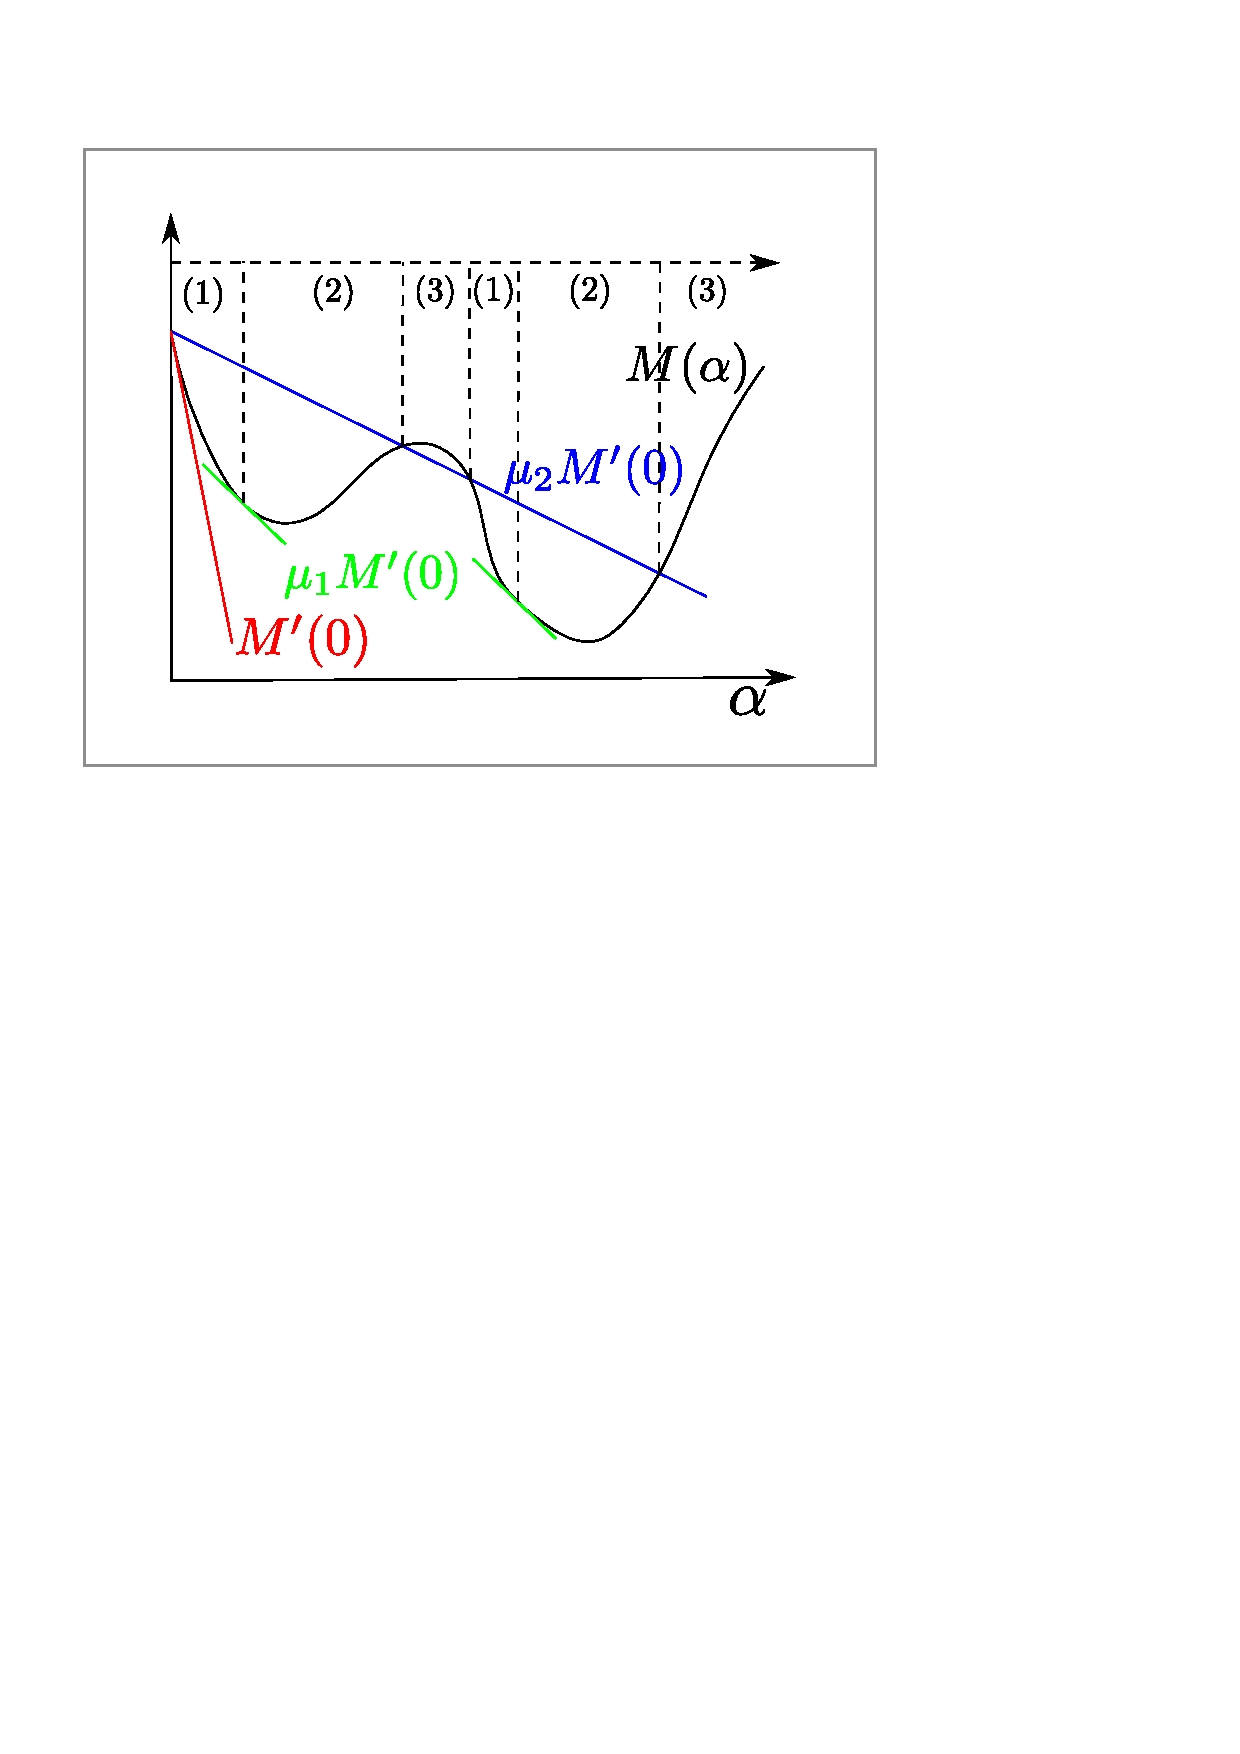
\includegraphics[width=0.7\textwidth]{line-search.pdf}
  \caption{Illustration of the choice made by the Wolfe line-search for values of $\alpha$}
\label{fig:Wolfe}
\end{figure}

The Wolfe line-search is popular, but it requires the computation of the derivative of the merit function, which can be prohibitively expensive in some cases, including in posture generation for robotics problems, where the derivatives are usually expensive.
Other line-search methods exist that do not require the derivative of $M$ for $\alpha\neq0$. For example the Goldstein and Price, or the Armijo methods.

\subsubsection{The filter method}
\label{ssub:the_filter_method}
The decision to accept on not a step generated by the QP can be made using a Filter approach instead of the Wolfe line search, as introduced by Fletcher in~\cite{fletcher:mathprog:2000}.
The goal of that method is to minimize the cost function $f(x)$ and the constraint violation $h(x)$ separately.
A step is accepted if it improves at least one of the function or the constraint violation.
\begin{equation}
  h(x) = \sum\limits_{k\in E} |c_k(x)| + \sum\limits_{k\in I} \max(0, -c_k(x))
\end{equation}

Denoting $h_i = h(x_i)$ and $f_i = f(x_i)$, we define the notion of domination as follows:
\begin{definition}
  \begin{equation}
    p_i\ \text{dominates }p_j \Leftrightarrow \left\{
        \begin{array}{l}
    f_i < f_j \\
    h_i < h_j
  \end{array}  \right.
  \end{equation}
\end{definition}

The filter maintains a list of pairs $p_i=\{f_i, h_i\}$ such that no pair dominates any other pair.
When a new point $x$ is submitted to the filter for acceptance, the values $f(x)$ and $h(x)$ are computed and the pair $p = \{f(x), h(x)\}$ is compared to every pair $p_i$.
If there is at least one pair $p_i$ in the filter that dominates $p$, the point is refused.
Otherwise, no pair of the filter dominates $p$, then $p$ is accepted and added to the filter.
Once $p$ is added to the filter, any pair in the filter that is dominated by $p$ is removed from it to ensure to keep a list of pairs non-dominated by each other in the filter.
In order to ensure global convergence, this method requires several refinements as explained in~\cite{fletcher:mathprog:2000}.
First, it needs to avoid accepting pairs that are excessively close to each other. For that, the domination criterion is modified with a sloping envelope, as proposed in Chin~\cite{chin:mathprog:2003}.
The sloping envelope definition takes user defined parameters $\beta$ and $\gamma$ in $[0,\ 1]$.

\begin{definition}
  \begin{equation}
    p_i\ \text{dominates }p_j \Leftrightarrow \left\{
        \begin{array}{l}
    f_i < f_j - \gamma h\ \\
    h_i < \beta h_j
  \end{array}  \right.
  \end{equation}
\end{definition}

\begin{figure}
  \centering
  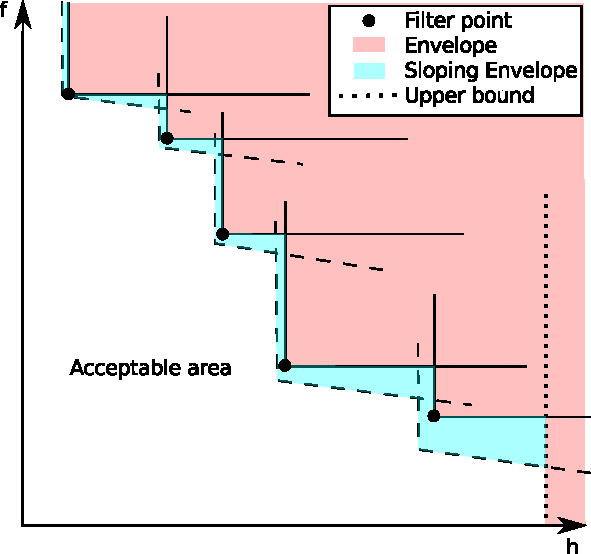
\includegraphics[width=0.7\textwidth]{filter.pdf}
  \caption{Representation of a filter with sloping envelope}
\label{fig:Filter}
\end{figure}

Another basic necessary improvement is to set an upper bound to the constraint violation, to avoid having the algorithm generate points that minimize the cost function while completely violating the constraints.

A representation of the filter method is given in figure~\ref{fig:Filter}

The filter method is convenient because it does not require the same complicated updates as can be found in penalty based methods where the penalty parameter needs to be updated regularly.
Also, with the filter method, no derivative computation is required.
That method is generally more permissive than merit-based method in the sense that it refuses fewer points.

The filter method, as well as the merit function based methods, can be used in line-search and trust-region algorithms.

\subsubsection{The Trust-Region Strategy}
\label{ssub:the_trust_region_strategy}
The Trust Region strategy is based on the idea that at any iterate $x_k$ the quadratic model made of the problem and fed to the QP solver can only be trusted to be relevant is a finite region around the iterate.
That region is called the trust region and its size is usually governed by a single positive parameter $\rho_k$ that can evolve along the optimization process.
This translates in a modified QP to solve at each iteration.
A boundary constraint describing the trust region is added to the problem.
At each step, the modified problem writes as:

\begin{equation}
  \begin{array}{ll}
    \minimize\limits_{z\in \mathbb{R}^n}{} & \frac{1}{2}z^T\nabla_{xx}^2Hz + \sum_{i\in\mathcal{U}}{\nabla c_i(x_k)}^T z \\
    \text{subject to } & {\nabla c_i(x_k)}^T z+c_i(x_k)=0,\ i\in \mathcal{F} \\
                       & {\nabla c_i(x_k)}^T z+c_i(x_k)\geq 0,\ i\in I\\
                       & |z|<\rho_k
  \end{array}
\label{approx_QP_TR}
\end{equation}

Once a solution $z$ of~\ref{approx_QP_TR} is found, the potential next iterate $x_{k+1} = x_k + z$ is checked against the acceptance criterion (should it be a merit function or a filter or other).
If it is accepted, that means that our current model is good, we move to the next step with $x_{k+1} \leftarrow x_k + z$, and the size of the trust region can be augmented based on some heuristics.
Otherwise, the iterate is refused, the model is less good than expected, the size of the trust region is reduced based on some heuristics (e.g. $\rho_{k+1}\leftarrow\rho_k /2$) and the problem~\ref{approx_QP_TR} is solved again with the new value of $\rho_{k+1}$.
This is repeated until a satisfying point is found, or until an infeasible problem is found.

\begin{figure}
  \centering
  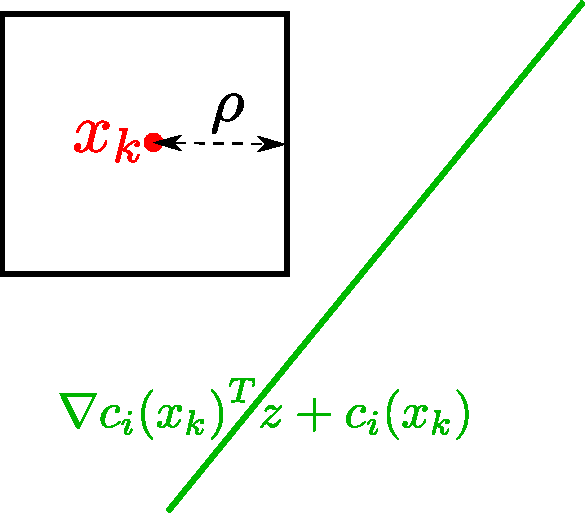
\includegraphics[width=0.4\textwidth]{trust_region_incompatible.pdf}
  \caption{Constraint incompatibility generated by trust region approach}
\label{fig:TR_incompatible}
\end{figure}

With this approach, a problem that often arises is the generation of infeasible problems.
The reduction of the size of the trust region can lead to an incompatible set of constraints.
For example, with a single constraint, as illustrated in figure~\ref{fig:TR_incompatible}.
The linearisation of the constraint is represented by the green line, and the trust region by the black rectangle.
If $\rho$ is too small, there is no intersection between the linearization of the constraint and the trust region.
The QP is then infeasible.
An obvious solution for that would be to increase the size of the trust region, but that goes against the core idea of the trust region strategy and it would harm the convergence properties of the algorithm.
A more appropriate solution is to enter a restoration phase when that event occurs.
The purpose of a restoration phase is to reduce the infeasibility of a problem by relaxing infeasible constraints without regards for the cost function.
The restoration phase is exited once a feasible point is found, and the course of the SQP is continued from that point.

\subsection{Restoration phase}
\label{sub:restoration_phase}

As we stated previously, a restoration phase is entered when an infeasible problem is found by the trust region strategy.
The goal of the restoration is to find a solution to the following problem:

\begin{equation}
    \text{Find $x\in\mathbb{R}^n$ such that }
    \left\{
    \begin{array}{l}
      c_i(x)=0,\ i\in E \\
      c_i(x)\geq 0,\ i\in I\\
      |z|<\rho_k
    \end{array}
    \right.
\label{eq:resto_NL}
\end{equation}

The restoration phase proceeds in a similar way to the original SQP algorithm described earlier.
At each step, an approximated QP is solved, then its result is compared to an acceptance criterion, if it is accepted, the trust region can be increased and the algorithm continues.
Otherwise, the trust region is reduced and the problem is solved again.
The acceptance criterion must be tailored for the restoration problem, meaning that it is based on the values of the cost function of the restoration problem and of its constraints.
The big difference comes from the way the quadratic problem is constructed during this phase.

During a restoration phase step, the first action is to estimate the sets $\mathcal{F}$ and $\mathcal{I}$ of feasible  and infeasible constraints.
This is done by solving the linearization of problem~\Eqref{eq:resto_NL} as presented in~\Eqref{eq:FP}.
Each equality constraint is cut in 2 inequality constraints.

\begin{equation}
  \text{Find $z\in\mathbb{R}^n$ such that }
  \left\{
  \begin{array}{l}
    {\nabla c_i(x_k)}^T z+c_i(x_k)\geq 0,\ i\in E \\
    -{\nabla c_i(x_k)}^T z-c_i(x_k)\geq 0,\ i\in E \\
    {\nabla c_i(x_k)}^T z+c_i(x_k)\geq 0,\ i\in I\\
    |z|<\rho_k
  \end{array}
  \right.
\label{eq:FP}
\end{equation}

The resolution of that FP gives the lists $\mathcal{F}$ and $\mathcal{I}$.
If the list of infeasible constraints is empty, the problem is feasible, so the restoration phase is exited to return to the main SQP algorithm.
The restoration QP to solve is built based on those lists.
The infeasible constraints are removed from the constraint set and the expression of their violation is added to the cost function, while the feasible constraints remain in the constraint list.
This results in a problem like~\ref{rest_SQP} to solve.
(Note that the indexes of the constraints are modified to account for the duplication of the equality constraints)

\begin{equation}
  \begin{array}{ll}
    \minimize\limits_{z\in \mathbb{R}^n}{} & \frac{1}{2} z^T Hz - \sum\limits_{i\in\mathcal{I}}{\nabla c_i(x_k)}^T z \\
    \text{subject to } & {\nabla c_i(x_k)}^T z+c_i(x_k)\geq 0,\ i \in \mathcal{F} \\
                       & |z|<\rho_k
  \end{array}
\label{rest_SQP}
\end{equation}

This problem is solved by a QP solver, its result is checked against an acceptance criterion, based on that, the trust region is enlarged or reduced, and we go back to solving the FP\@.

In the restoration phase, special care must be taken in the computation of the matrix H, that represents the Hessian of the Lagrangian of a problem that changes at each iteration.
One possible approach is to compute it as the sum of the Hessians of all the individual constraints, and those can be computed exactly or with a quasi-newton approximation.


\subsection{Quasi-Newton Approximation}
\label{sub:quasi_newton_approximation}

In the SPQ algorithm, it is necessary to have access to the Hessian of the Lagrangian $\nabla_{xx}^2\mathcal{L}$ to be able to devise the QP subproblem to solve.
%For some strategies like the Line-Search, it is necessary that $\nabla_{xx}^2\mathcal{L}$ is definite positive.
Sometimes the exact Hessian of the problem is not positive definite.
Also, it is often difficult or computationally expensive to compute an exact Hessian of the Lagrangian.
Since we are following an iterative process, it is not necessary to have an exact knowledge of the Hessian and using an approximation of it is usually enough.
Also, an approximate Hessian is in most cases less expensive to compute than the exact one.

The idea behind computing an approximate Hessian is that, starting from an initial approximate Hessian $B_0$, we compute at each iteration an update to the approximate Hessian based on the values and first order derivatives of the Lagrangian.
This update aims at capturing some curvature information about the Hessian by evaluating the evolution of the gradient along the latest step.
At step $k$, the Hessian update is a function of $s_k$ and $y_k$:
\begin{equation}
  s_k = x_{k+1}-x_k,\ \ \ \
  y_k = \nabla_x\mathcal{L}(x_{k+1}, \lambda_{k+1}) - \nabla_x\mathcal{L}(x_{k}, \lambda_{k+1})
\end{equation}

The two most famous Hessian update strategies are called the BFGS (Broyden–Fletcher– Goldfarb–Shanno) and the SR1(Symmetric Rank 1) updates.
BFGS is a rank 2 update while SR1 is rank 1.

The most basic formulas for the BFGS update is the following:

\begin{equation}
\label{BFGS}
  B_{k+1} = B_k - \frac{B_k s_k s_k^T B_k}{s_k^T B_k s_k} + \frac{y_k y_k^T}{s_k^T y_k}
\end{equation}

Note that using a BFGS update requires that $s_k$ and $y_k$ satisfy the curvature condition: $s_k^T y_k>0$.
If that condition does not hold, then the value of $y_k$ is modified, which gives rise to the Damped BFGS update, which guarantees to keep $B_k$ definite positive:

\begin{equation}
\label{damped_BFGS}
\begin{split}
  \theta_k =
  \left\{
      \begin{array}{ll}
      1 & \text{if } s_k^T y_k \geq 0.2 s_k^T B_k s_k \\
      \frac{0.8 s_k^T B_k s_k}{s_k^T B_k s_k-s_k^T y_k} & \text{if } s_k^T y_k \geq 0.2s_k^T B_k s_k \\
      \end{array}
      \right.\\
      r_k = \theta_k y_k + (1-\theta_k) B_k s_k\\
      B_{k+1} = B_k-\frac{B_k s_k s_k^T B_k}{s_k^T B_k s_k} + \frac{r_k r_k^T}{s_k^T r_k}
\end{split}
\end{equation}

The SR1 update is computed with the following formula:

\begin{equation}
\label{SR1}
B_{k+1} = B_k + \frac{(y_k-B_k s_k){(y_k-B_k s_k)}^T}{{(y_k-B_k s_k)}^T s_k}
\end{equation}

Both those formulas proved to be efficient in some cases. It is not yet clear in which cases one is better than the other.

\section{Conclusion}
This section gives a general introduction to nonlinear constrained optimization without regards for specificities of robotics problem or formulations on manifolds, which are topics considered in the core of this thesis.



\end{appendices}

% *************************************** Index ********************************
\printthesisindex % If index is present

\end{document}
